\documentclass[a4paper, 12pt]{article}
\usepackage[a4paper, total={6in, 8in}]{geometry}
\geometry{
	a4paper,
	left = 1.5 cm,
	right = 1.5 cm,
	top = 2cm,
}
\usepackage[T1]{fontenc}
\usepackage{pythontex}
\usepackage{hhline}
\usepackage{array,booktabs}
\newcolumntype{M}[1]{>{\centering\arraybackslash}m{#1}}
\usepackage[table]{xcolor}
\usepackage{caption}
\usepackage{makecell}
\usepackage{lipsum}
\usepackage{pifont}
\usepackage{amssymb}
\usepackage{amsmath}
\usepackage[utf8]{inputenc}
\usepackage[italian]{babel}
\usepackage{graphicx}
\graphicspath{ {./images/} }
\usepackage{spverbatim}
\usepackage{float}
\usepackage{url}
\usepackage{xstring}
\usepackage{hyperref}
\usepackage{xcolor}
\definecolor{linkcolor}{RGB}{1,1,87}
\hypersetup{
    colorlinks,
    citecolor=black,
    filecolor=black,
    linkcolor=linkcolor,
    urlcolor=blue
}
\usepackage{fancyvrb,newverbs,xcolor}
\definecolor{cverbbg}{gray}{0.93}
\definecolor{cellcolor}{RGB}{165,194, 242}
\usepackage{xifthen}
\usepackage{multirow}

\newcommand{\sysroot}[0]{\key{\%SYSTEMROOT\%}}
\newcommand{\makesub}[1]{%
  \saveexpandmode\noexpandarg
  \StrSubstitute{#1}{\_}{_}[\temp]%
  \restoreexpandmode%
}

\newcommand{\target}[1]{%
  \makesub{#1}%
  \hypertarget{\temp}{}%
}

\newcommand{\attach}[1]{%
  \makesub{#1}%
  \hyperlink{\temp}{\emph{#1}}%
}
\newcommand{\attachcode}[1]{%
  \makesub{#1}%
  \hyperlink{\temp}{\code{#1}}%
}

\newcommand{\code}[1]{\colorbox{cverbbg}{\texttt{\StrSubstitute{#1}{_}{\_}}}}

\newcommand{\linux}{\textit{Linux}}
\newcommand{\win}{\textit{Windows}}
\newcommand{\nota}[1]{\textbf{Nota}: #1}
\newcommand{\memo}[1]{\textbf{Memo}: #1}
\newcommand{\esempio}[1]{\textbf{Esempio}: #1}
\newcommand{\tbs}{\textbackslash}
\newcommand{\ghidra}{\emph{Ghidra}}
\newcommand{\ollydb}{\emph{OllyDB}}
\newcommand{\Null}{\code{NULL}}
\newcommand{\dll}{\emph{DLL}}
\newcommand{\api}{\emph{API}}
\newcommand{\key}[1]{\texttt{\StrSubstitute{#1}{_}{\_}}}

\newcommand{\paramtable}[2][]{%
\ifthenelse{\isempty{#2}} {\input{|"/home/luca/Scrivania/MA/homeworks/homework-04/report/scripts/generate_param_table.py '#1'"}} {\input{|"/home/luca/Scrivania/MA/homeworks/homework-04/report/scripts/generate_param_table.py '#1' '#2'"}}%
}
\newcommand{\image}[1]{\input{|"/home/luca/latex_scripts/add_image.py '#1'"}}

\newcommand{\eax}[0]{\key{EAX}}
\newcommand{\ebx}[0]{\key{EBX}}
\newcommand{\ecx}[0]{\key{ECX}}
\newcommand{\edx}[0]{\key{EDX}}
\newcommand{\ebp}[0]{\key{EBP}}
\newcommand{\esp}[0]{\key{ESP}}
\newcommand{\esi}[0]{\key{ESI}}
\newcommand{\edi}[0]{\key{EDI}}
\newcommand{\struct}[3]{%
\begin{tabular}{|c|c|}%
\hline%
following byte address & #1 \\%
\hline%
current byte & #2 \\%
\hline%
remaining bits & #3 \\%
\hline%
\end{tabular}%
}

\newenvironment{myverb}
 {\SaveVerbatim{cverb}}
 {\endSaveVerbatim
  \flushleft\fboxrule=0pt\fboxsep=.5em
  \colorbox{cverbbg}{%
    \makebox[\dimexpr\linewidth-2\fboxsep][l]{\BUseVerbatim{cverb}}%
  }
  \endflushleft
}

\setcounter{tocdepth}{4}
\setcounter{secnumdepth}{4}
\setlength\parindent{0pt}

\begin{document}\sloppy
  
\title{
  \textbf{
    \emph{Relazione homework 4}
  }
}  
\author{Luca Mastrobattista\\ Matricola: 0292461}
\date{}
\maketitle

\tableofcontents
\newpage
\section{Traccia dell'homework}
\subsection{Testo}
Analizzare il programma eseguibile hw4.ex\_ contenuto
nell'archivio hw4.zip (password: "AMW21").
Determinare ogni possibile informazione riguardo alle
funzionalita' del programma, riassumendole in un documento
che riporti anche la metodologia adottata ed i passi logici
deduttivi utilizzati nel lavoro di analisi.\\
ATTENZIONE: IL MALWARE E' REALE E PUO' PROVOCARE DANNI AI
SISTEMI INFORMATICI SE NON OPPORTUNAMENTE CONTROLLATO E
MONITORATO.

\subsection{Scadenza}
Tre giorni prima della data d'appello in cui si
intende sostenere l'esame orale.

\subsection{Consegna}
Documento in formato PDF inviato come allegato ad
un messaggio di posta elettronica all'indirizzo del docente
("$<$cognome$>$@uniroma2.it"), con subject:
"[AMW21] HW4: $<$matricola studente$>$"

\newpage
\section{Ambiente di lavoro}
Il file eseguibile è stato caricato su Ghidra istallato su un sistema operativo Linux. \\
L'ambiente controllato di utilizzo è un sistema operativo Windows 10 virtualizzato con il software \emph{VirtualBox}, in cui sono istallati gli strumenti di monitoraggio.


\subsubsection{Riepilogo risultati dell'import}
\begin{figure}[H]
\centering 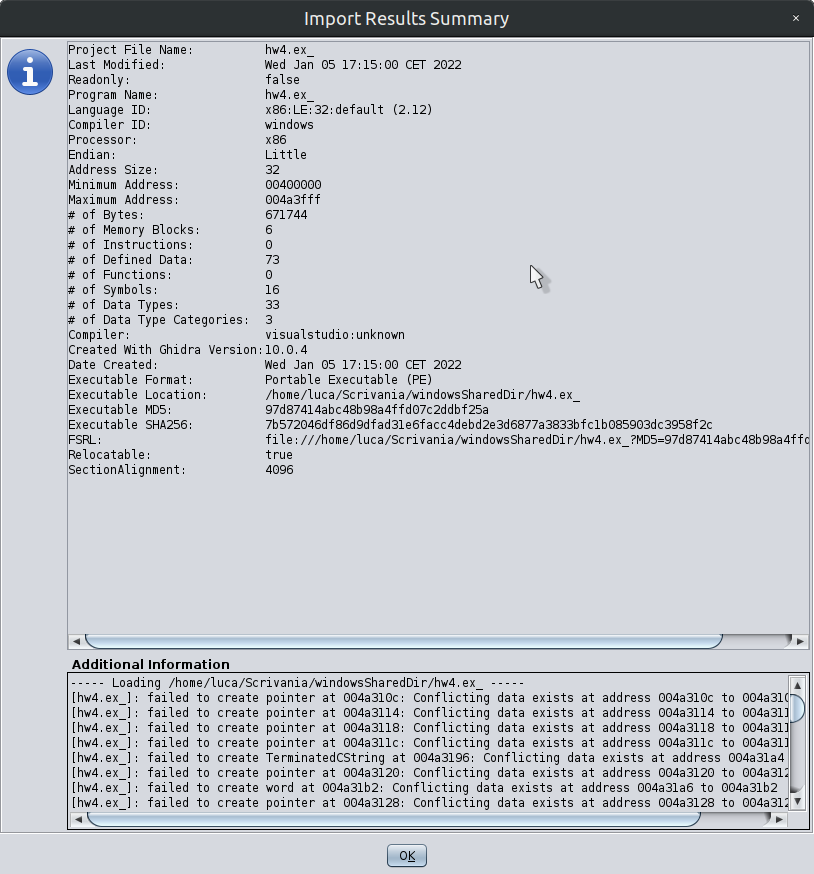
\includegraphics[width=\textwidth]{import}
\end{figure}
\subsubsection{Informazioni aggiuntive}
\begin{spverbatim}
----- Loading /home/luca/Scrivania/windowsSharedDir/hw4.ex_ -----
[hw4.ex_]: failed to create pointer at 004a310c: Conflicting data exists at address 004a310c to 004a310f
[hw4.ex_]: failed to create pointer at 004a3114: Conflicting data exists at address 004a3114 to 004a3117
[hw4.ex_]: failed to create pointer at 004a3118: Conflicting data exists at address 004a3118 to 004a311b
[hw4.ex_]: failed to create pointer at 004a311c: Conflicting data exists at address 004a311c to 004a311f
[hw4.ex_]: failed to create TerminatedCString at 004a3196: Conflicting data exists at address 004a31a4 to 004a31a5
[hw4.ex_]: failed to create pointer at 004a3120: Conflicting data exists at address 004a3120 to 004a3123
[hw4.ex_]: failed to create word at 004a31b2: Conflicting data exists at address 004a31a6 to 004a31b2
[hw4.ex_]: failed to create pointer at 004a3128: Conflicting data exists at address 004a3128 to 004a312b
[hw4.ex_]: failed to create word at 004a31c2: Conflicting data exists at address 004a31b4 to 004a31c2
[hw4.ex_]: failed to create pointer at 004a3130: Conflicting data exists at address 004a3130 to 004a3133
[hw4.ex_]: failed to create pointer at 004a3138: Conflicting data exists at address 004a3138 to 004a313b
[hw4.ex_]: failed to create word at 004a31da: Conflicting data exists at address 004a31ce to 004a31da
Delay imports detected...
Searching for referenced library: USER32.DLL ...
Unable to find external library: USER32.DLL
Searching for referenced library: SHELL32.DLL ...
Unable to find external library: SHELL32.DLL
Searching for referenced library: CMUTIL.DLL ...
Unable to find external library: CMUTIL.DLL
Searching for referenced library: SHIMENG.DLL ...
Unable to find external library: SHIMENG.DLL
Searching for referenced library: KERNEL32.DLL ...
Unable to find external library: KERNEL32.DLL
Finished importing referenced libraries for: hw4.ex_
  [CMUTIL.DLL] -> not found
  [KERNEL32.DLL] -> not found
  [SHELL32.DLL] -> not found
  [SHIMENG.DLL] -> not found
  [USER32.DLL] -> not found

\end{spverbatim}

\newpage
\section{Analisi}

\subsection{Basic static (code) analysis}
Utilizzando il comando \key{strings} da terminale \linux{}, si nota come le sembrino essere cifrate. È ragionevole pensare che il programma sia stato impacchettato. Una conferma la troviamo analizzando il file con il tool \textit{PEiD}:\\
\begin{minipage}{0.4\textwidth}
\begin{figure}[H]
\centering 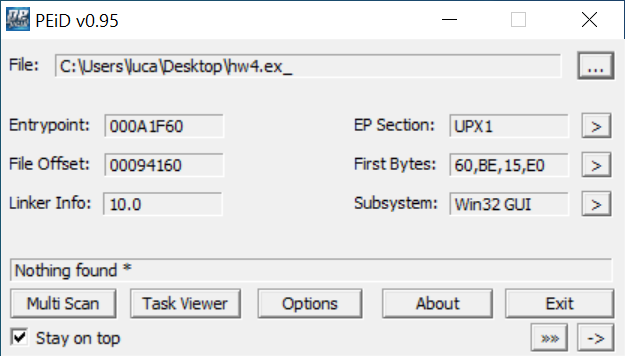
\includegraphics[width=\textwidth]{peid}
\end{figure}
\end{minipage}\hfill
\begin{minipage}{0.4\textwidth}
\begin{figure}[H]
\centering 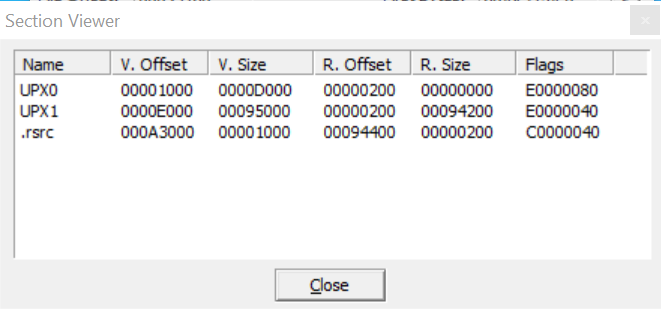
\includegraphics[width=\textwidth]{peid2}
\end{figure}
\end{minipage}\\

\noindent Nella sezione \key{EP Section} notiamo \key{UPX1}: significa che l'eseguibile è stato effettivamente impacchettato con il \textit{packer} open source \key{UPX}, che viene però identificato solo dopo aver eseguito una \textit{Deep scan}: \key{UPX 0.89.6 - 1.02 / 1.05 - 2.90 -> Markus \& Laszlo}. Si può quindi scompattare automaticamente eseguendo \code{upx -d hw4.ex_ -ounpacked.ex_} sul sistema host. Il file ottenuto è leggermente più grande del file originale: potrebbe aver funzionato: eseguendo nuovamente il comando \code{strings} sul file \textit{unpacked.ex\_} si possono leggere molte stringhe note, come ad esempio \key{"kernel32.dll"}. Il file ottenuto, però, non risulta eseguibile. 

\subsection{Basic dynamic (behaviour) analysis}
Eseguendo il malware su una macchina virtuale \win{} non collegata alla rete, si può osservare che questo si tratta in realtà di un \textit{ransomware}: dopo aver terminato la sua esecuzione, vengono creati due nuovi file, un file \textit{asasin.html} e un file \textit{asasin.bmp}, che riportano la stessa scritta; si tratta delle istruzioni da seguire per ottenere la chiave per decifrare i dati. L'immagine viene anche impostata come sfondo. Inoltre, per ogni file che viene criptato dal malware viene creato un file in formato \textit{asasin}.

\subsection{Advanced analysis}
Cerchiamo per prima cosa di recuperare l'eseguibile originale. Come detto, usando \textit{upx} il programma di output non risulta eseguibile. Si procede quindi in altri modi.

\subsubsection{Ricerca dell'OEP}
Utilizzando \ghidra{} per identificare i vari \key{JMP}, notiamo che ce n'è qualcuno veramente grande:
\begin{figure}[H]
\centering 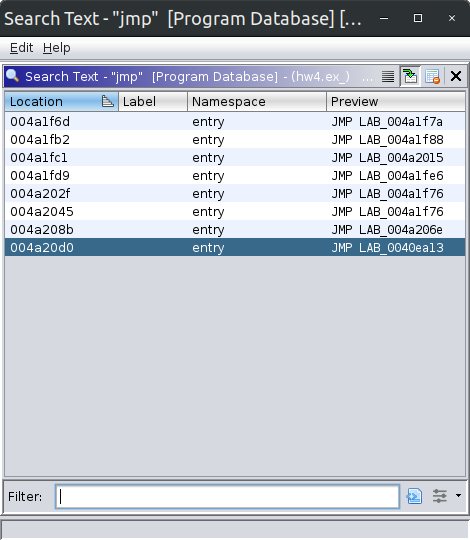
\includegraphics[scale=0.4]{jumps}
\end{figure}
\noindent
In particolare, il salto evidenziato è veramente grande, e potrebbe essere effettivamente il nostro \textit{tail jump}. Tuttavia, per una conferma, sfruttiamo \ollydb{}: il codice, infatti, utilizza nell'\textit{entry point} dello stub l'istruzione \code{PUSHAD} e si può quindi verificare che i registri verranno recuperati prima del salto evidenziato. Il codice si interrompe proprio prima di quel salto: si può concludere che l'\textit{OEP} sia effettivamente all'indirizzo \key{0x0040ea13}.

\subsubsection{Fare il \textit{dump}}
Utilizzando il plugin \textit{OllyDump}, si prova a questo punto a eseguire il dump di memoria con tutti e 3 i metodi: 
\begin{enumerate}
\item ricreando la \textit{IAT} tramite istruzioni di \code{JMP} e \code{CALL}
\item ricreando la \textit{IAT} tramite il nome delle \api{} invocate
\item senza ricreare la \textit{IAT}
\end{enumerate}
Entrambi i primi due metodi ricostruiscono l'\textit{IAT} correttamente: provando ad invocarli, infatti, si verifica lo stesso comportamento del malware originale. Si procede ad analizzare il file eseguibile generato dal metodo 1.

\subsection{Advanced analysis - dump-method1.exe}
Il programma fa una serie di invocazioni alla funzione \code{IsBadStringPtrW} che ritorna \key{0} se non ci sono errori, passando come parametri:
\begin{itemize}
\item \key{"lwpqabklbeiutlcti", 17}. Valore di ritorno \key{0}.
\item \key{"lwpqabklbeiutlcti", 17}. Valore di ritorno \key{0}.
\item \key{"lwpqabklbeiutlcti", 17}. Valore di ritorno \key{0}.
\item \key{"vickhgfqkhpdvlnva", 17}. Valore di ritorno \key{0}.
\end{itemize}
Capire bene pure questa cosa.\\

\subsubsection{Primo VirtualAlloc}
All'indirizzo \key{0040699a} si invoca indirettamente la funzione \key{VirtualAlloc}, allocando 688h bytes, cioè 1672. I parametri di invocazione sono i seguenti:
\begin{itemize}
\item addr = \Null{}: i bytes vengono allocati su una qualsiasi zona di memoria disponibile. Significa che ad ogni esecuzione questo potrebbe cambiare.
\item size = 688h = 1672 bytes allocati.
\item AllocType = \key{MEM_COMMIT}
\item Protect = \key{PAGE_EXECUTE_READWRITE} 
\end{itemize}
Questa memoria viene scritta nelle successive istruzioni, partendo dall'indirizzo \key{004069ac}
\begin{myverb}
            LAB_004069ac 
004069ac ff 31      PUSH   dword ptr [ECX]
004069ae 58         POP    EAX
004069af f8         CLC
004069b0 83 d1 04   ADC    ECX,0x4
004069b3 f7 d0      NOT    EAX
004069b5 f8         CLC
004069b6 83 d8 21   SBB    EAX,0x21
004069b9 8d 40 ff   LEA    EAX,[EAX + -0x1]
004069bc 29 f0      SUB    EAX,ESI
004069be 29 f6      SUB    ESI,ESI
004069c0 29 c6      SUB    ESI,EAX
004069c2 f7 de      NEG    ESI
004069c4 89 03      MOV    dword ptr [EBX],EAX
004069c6 8d 5b 04   LEA    EBX,[EBX + 0x4]
004069c9 8d 7f fc   LEA    EDI,[EDI + -0x4]
004069cc 83 ff 00   CMP    EDI,0x0
004069cf 75 db      JNZ    LAB_004069ac
\end{myverb}
Si sta leggendo il valore in \key{ECX}, lo si decodifica e infine lo si scrive nell'area di memoria allocata. Il valore iniziale di \key{ECX} è l'indirizzo \key{00496000}, in \key{EBX} c'è l'indirizzo restituito dall'invocazione della \key{VirtualAlloc} e in \key{EDI} il valore \key{688h}, cioè il numero di bytes allocati: si tratta di un contatore dei bytes che devono ancora essere scritti. Il codice appena scritto viene poi invocato. \\

\subsubsection{Codice decodificato}
Si esegue quindi il codice nella zona di memoria appena allocata ma, all'offset \key{1e} viene invocata una funzione che esegue \key{PUSHAD}: il programma potrebbe essere impacchettato più volte. \\
All'indirizzo \key{006e064c} vengono caricati gli indirizzi di: \key{HeapAlloc}, \key{HeapFree}, \key{GetTickCount}.\\
All'offset \key{65h} dell'indirizzo ottenuto dalla prima invocazione di \key{VirtualAlloc} ce n'è un'altra, sempre di \key{688h} bytes. In questa zona di memoria viene copiato tutti i bytes contenuti nella prima. Quando viene eseguito il \key{RETN}, il codice continua all'offset \key{79h} del nuovo indirizzo restituito, perché questo era stato precedentemente inserito sulla cima dello \textit{stack}. \\ Una cosa che è possibile notare è che i bytes a partire dall'indirizzo \key{004069da}, indirizzo in cui si invoca il codice decodificato, vengono modificati proprio da questo blocco di codice. La sostituzione di quei bytes avviene all'offset \key{113h} dell'indirizzo ottenuto dalla prima invocazione di 	\key{VirtualAlloc}.

\subsection{Secondo VirtualAlloc}
Il codice inizia con l'invocazione della funzione all'offset \key{605h}. All'offset \key{8e} viene invocata una nuova \key{VirtualAlloc}, che però alloca molti bytes in più delle precedenti due: ne alloca infatti \key{83a00h}, cioè \key{539136}. All'offset \key{9f}, invece, viene invocata una funzione che esegue \key{PUSHAD} e \key{POPAD} rispettivamente all'inizio e alla fine della funzione. Potrebbe essere stato impacchettato ancora un'altra volta.\\
In seguito viene invocata la funzione \key{VirtualProtect} con i seguenti parametri:
\begin{itemize}
\item \key{address=00400000}
\item \key{size=400}
\item \key{newProtect=PAGE_READWRITE}
\item \key{pOldProtect=0019FEFC}: è l'indirizzo dove viene memorizzata la precedente protezione. Dopo l'invocazione, contiene il valore \key{2}, che corrisponde a \key{PAGE_READONLY}.
\end{itemize}
I \key{400h} bytes successivi all'indirizzo \key{00400000} vengono sovrascritti con quelli appena inseriti nell'indirizzo ottenuto dalla terza invocazione di \key{VirtualAlloc}. Al termine dell'operazione, viene ripristinata la protezione sui bytes sovrascritti con una nuova invocazione di \key{VirtualProtect}, che reimposta la protezione a \key{PAGE_READONLY}.\\
Dopo una serie di operazioni che non sono ben chiare, viene invocata nuovamente la funzione \key{VirtualProtect}, all'offset \key{10c}. Cambia la protezione dei 495616 (\key{79000h}) bytes a partire dall'indirizzo \key{401000}, impostandola su \key{PAGE_READWRITE}: sta per scrivere questi bytes. Per prima cosa, infatti, li imposta tutti a 0, poi scrive al suo interno gli \key{78600h} bytes contenuti dall'offset \key{400h} in poi del terzo indirizzo virtuale. Dopo la scrittura, viene di nuovo cambiata la protezione in \key{PAGE_EXECUTE_READ} con \key{VirtualProtect}. \\
Il codice continua ripetendo lo stesso meccanismo, partendo però sta volta da un  offset diverso del terzo indirizzo di virtual alloc: prima si partiva dall'indirizzo che puntava alla stringa \key{.text}, questa volta la stringa puntata è \key{.rdata}. Si stanno decodificando le varie sezioni. Si prosegue infatti copiando la sezione \key{.data}, \key{.reloc} e \key{.cdata}.\\
Il codice continua invocando virtualProtect sui \key{1c4h (452)} bytes che partono dall'indirizzp \key{47a0bc}. Viene poi invocata \key{GetProcAddr} per recuperare l'indirizzo della funzione \key{OpenMutexA} da \key{Kernel32.dll}, che viene poi salvato all'indirizzo \key{47a0bc}. Sempre con questo meccanismo, vengono caricare e memorizzate negli indirizzi successivi diverse funzioni; sono in tutto 113. Il codice continua reimpostando la VirtualProtect a \key{PAGE_READONLY}. Dopo aver finito di caricare le \api{} da \key{Kernel32}, inizia a caricare quelle di \key{Advapi32.dll}. Possiamo quindi concludere che questa funzione effettua il caricamente di tutte le \api{} di tutte le librerie.\\
Il codice continua con \code{PUSH dword ptr FS:[30]}, all'indirizzo \key{base_address2 + 0x149}: si sta mettendo sullo stack la struttura \textit{PEB}. Bisogna stare attenti: sappiamo infatti che all'offset 2 di questa struttura c'è il campo \textit{being\_debugged}. Si sono quindi inseriti dei breakpoints harware sul singolo byte, sulla word e sulla dword, in modo da catturare qualsiasi tipo di accesso al byte. Tuttavia questa struttura è utilizzata per accedere alla struttura dati \key{PEB_LDR_DATA}, all'offset \key{0xc}. In particolare, si accede alla lista \key{InLoadOrderLinks} all’offset \key{0xc}, ordinata secondo l'ordine di caricamento. Si accede al campo \key{DLLbase} del primo elemento e lo si confronta con l'\textit{entry point} del programma iniziale: \key{400000}. Il confronto da esito positivo (perché?).\\
All'offset \key{0x187} viene invocata la \key{VirtualFree} sui bytes allocati dalla terza \key{VirtualAlloc}; i parametri infatti sono i seguenti:
\begin{itemize}
\item \key{address = base_address3}
\item \key{size = 83a00}
\item \key{FreeType = MEM_DECOMMIT}
\end{itemize}
Viene poi invocata una funzione \key{FUN_00000431} che a runtime non esegue nulla, poi si invoca \key{FUN_000004f5} che invoca \key{GetModuleHandle} con parametro \Null{}: si sta recuperando un \textit{handle} al file usato per creare il processo corrente. Successivamente, un'altra invocazione che a runtime non fa altro che eseguire \key{PUSHAD} e \key{POPAD}, all'offset \key{199}. Infine, all'offset \key{1a0} c'è un invocazione che l'unica cosa che fa è eseguire una \key{CALL} all'indirizzo di ritorno, con \code{POP EAX} e \code{CALL EAX}. L'indirizzo recuperato dallo stack è \key{base_address2 + 0x1a5}. In quest'ultima funzione, viene eseguito un \key{JMP} che salta a \key{402d8f}: siamo saltati all'interno del nuovo \key{entry_point}: i bytes, infatti, sono diversi da quelli originali in quanto sono stati sovrascritti all'offeset \key{113}.\\
Viene invocata \key{GetStartupInfoW} e dopo \key{HeapSetInformation} con i seguenti parametri:
\begin{itemize}
\item \key{HeapHandle = NULL}
\item \key{HeapInformationClass = HeapEnableTerminationOnCorruption}. Enables the terminate-on-corruption feature. If the heap manager detects an error in any heap used by the process, it calls the Windows Error Reporting service and terminates the process. After a process enables this feature, it cannot be disabled. 
\item \key{HeapInformation = NULL}
\item \key{HeapInformationLength = 0}
\end{itemize} 
Gli ultimi due parametri sono fissi quando si usa \key{HeapEnableTerminationOnCorruption} come secondo parametro. All'indirizzo \key{00402c96} c'è \key{__heap_init} e altre funzioni di libreria. Tra queste, c'è \key{GetCommandLineA}, che restituisce in \key{EAX} il puntatore alla stringa ASCII contenente il path completo dell'eseguibile, compreso di apici: \key{"C:\tbs{}Users\tbs{}luca\tbs{}Desktop\tbs{}dump-method1.exe"}. In seguit si invoca \key{GetEnvironmentStringsA}: sta inizializzando l'ambiente. Alla fine, all'indirizzo \key{00402d37} viene invocata la funzione \key{FUN_0042c820}: è l'unica invocata ed è quindi il \key{main} del processo. \\

\target{FUN\_0042c820\_main}
\subsection{FUN\_0042c820\_main}
Questa esegue per prima cosa un \key{GetModuleHandle} con parametro \key{NULL}: sta recuperando, di nuovo, un \textit{handle} al file usato per creare il processo corrente.\\
La funzione invoca successivamente \attachcode{FUN_00477050_generate_key_and_files}. Quando questa funzione ritorna, si verifica che il valore di ritorno non sia 0: se lo è viene invocato \code{ExitProcess} con valore \key{-2}, altrimenti, invoca \attachcode{FUN_00429ea0} prima di terminare.

\target{FUN\_00477050\_generate\_key\_and\_files}
\subsection{FUN\_00477050\_generate\_key\_and\_files}
 esegue una serie di \key{JMP}, \key{NOP} e altre istruzioni che hanno lo stesso effetto di un \key{NOP}, come \code{LEA EAX, dword ptr [EAX]}. L'analisi dinamica e statica è resa quindi molto difficile e frustrante da questo meccanismo. \\
La funzione apre un ciclo per leggere tutti i bytes dell'eseguibile (da \key{400000} a \key{489000}) con le seguenti istruzioni, inizializzando \key{EAX = 400000} e \key{EDX = 488fe8}:
\begin{myverb}
   loop_start:
CMP EAX, EDX
JC check
   
   range_end:
<...>

   check:
MOV ECX, dword ptr [EAX]
TEST ECX, ECX
JZ increment
MOV ESI, ECX 
XOR ESI, 0x88bbdd8d
CMP dword ptr [EAX + 0x4], ESI
JNZ increment
XOR ECX, 0xddbca2b2
CMP dword ptr [EAX + 0x8], ECX
JZ pattern_found 	; <jmp to other stuff>

   increment:
INC EAX
JMP loop_start
\end{myverb}
Si esce dal ciclo con l'istruzione \code{JZ LAB_004777a2}, quindi solo se:
\[
\begin{cases}
\key{ECX} \neq \key{0x0} \\
\key{ECX XOR 0x88bbdd8d} = [\key{EAX + 4}]  \\
\key{ECX XOR 0xddbca2b2} = [\key{EAX + 8}]  \\
\end{cases}
\]
Dove con \key{ECX} si indicano i 4 bytes puntati da \key{EAX}, che viene incrementato nel ciclo. Cerchiamo quindi se si esce dal ciclo perché si sono controllati tutti i bytes del \textit{range} oppure perché le tre precedenti condizioni vengono ritrovate. Per farlo si piazza un breakpoint sulla prima istruzioni successiva al salto in \key{pattern_found}, cioè \key{477393}, e di \key{range_end}, cioè \key{4774a7}. Premendo \key{F9}, l'eseguibile si fermerà alla prima delle due istruzioni raggiunta. \\
Il primo brekpoint raggiunto è quello in \key{477393}: viene trovato il pattern quando \key{EAX = 488000}. Si ha infatti la seguente sequenza di bytes:
\begin{myverb}
[ EAX ]     = C8 3E C0 16 
[ EAX + 4 ] = 40 85 1D 9B
[ EAX + 8 ] = 15 82 62 A4
\end{myverb} 
e si può verificare facilmente che le tre condizioni precedenti sono tutte vere. \\
Nel blocco di codice seguente, all'indirizzo \key{477793}, si effettua una invocazione a \key{VirtualAlloc} con i seguenti parametri:
\begin{itemize}
\item addr = \key{NULL}
\item size = b07h = 2823 bytes allocati.
\item AllocType = \key{MEM_COMMIT | MEM_RESERVE}
\item Protect = \key{PAGE_READWRITE} 
\end{itemize}
Successivamente, si accede all'offset \key{30h} di \key{FS:[18]} per prenderne il secondo byte: si sta controllando se si è sotto un debugger. Evitato il controllo, il codice continua scrivendo i bytes allocati con il seguente ciclo:
\begin{myverb}
	loop_start:
MOV EAX, dword ptr [EBP + param2]
MOV CL, DL 
AND CL, 0x1f
ROL EAX, CL 
MOV ECX, dword ptr [EBP + param2]
ROR ECX, 0x3 
ADD EAX, ECX 
MOV ECX, EDX 
ROR ECX, 0xb
ADD ECX, 0x72462828
XOR EAX, ECX
MOV ECX, dword ptr [EBP + local10]
MOV dword ptr [EBP + param2], EAX 
LEA EAX, [EDX + EBX * 0x1]
MOV CL, byte ptr [ECX + EAX * 0x1]
XOR CL, byte ptr [EBP + param2]
MOV EBX, dword ptr [EBP, local_c]
INC EDX
MOV byte ptr [EAX], CL 
CMP EDX, ESI 
JC loop_start
\end{myverb}
Al termine del ciclo, c'è una nuova invocazione di \key{VirtualAlloc} all'indirizzo \key{477428}:
\begin{itemize}
\item addr = \key{NULL}
\item size = 6494h = 25748 bytes allocati.
\item AllocType = \key{MEM_COMMIT | MEM_RESERVE}
\item Protect = \key{PAGE_READWRITE} 
\end{itemize}
L'indirizzo di ritorno viene messo sullo stack all'indirizzo \key{EBP + c}, viene messo in \key{EDI} l'indirizzo di \key{VirtualFree} e viene invocata \attachcode{FUN_0046e870}.\\

Quando la precedente invocazione ritorna, il codice continua invocando \attachcode{FUN_0046E940} con i seguenti parametri:
\begin{itemize}
\item L'indirizzo restituito dalla \key{VirtualAlloc} a \key{477428}, l'ultima eseguita
\item Il valore \key{19fedc}
\item L'indirizzo restituito dalla \key{VirtualAlloc} a \key{477793}, la penultima in ordine cronologico
\end{itemize}

Quando la funzione ritorna, il codice continua invocando una \key{VirtualFree} all'indirizzo \key{47767f}.

\target{FUN\_0046e870}
\subsubsection{FUN\_0046e870}

Questa funzione mette dentro ai registri \key{ESI} e \key{ECX} rispettivamente gli indirizzi \key{483698} e \key{483970} prima di invocare la funzione \attachcode{FUN_0046d530_generate_alphabet}. I valori inseriti nei registri specificano le aree di memoria da scrivere. Quando quella funzione ritorna, ne viene invocata subito un'altra, per due volte: si tratta di \attachcode{FUN_0046d340}, passando i seguenti parametri: 
\begin{center}
\begin{tabular}{|c|c|c|}
\hline
{\cellcolor{cellcolor}} & {\cellcolor{cellcolor}} Prima invocazione & {\cellcolor{cellcolor}} Seconda invocazione \\
\hline
{\cellcolor{cellcolor}} Primo parametro: & \key{DAT_00483678} & \key{DAT_00483658} \\
\hline
{\cellcolor{cellcolor}} Secondo parametro: & \key{DAT_00483934} & \key{DAT_004838f8} \\
\hline
{\cellcolor{cellcolor}} Terzo parametro: & \key{0x3} & \key{0x1} \\
\hline
\end{tabular}
\end{center}
Dopo queste invocazione e aver scritto complessivamente i seguenti bytes, la funzione continua sovrascrivendone 2 e ritornando il valore \key{102h}.
\begin{center}
\begin{tabular}{|c|c|c|}
\hline
\multicolumn{3}{|c|}{\makecell{\key{FUN_0046d530_} \\ \key{generate_alphabet}}} \\[15pt]
\hline
Da & A & Bytes scritti \\
\hline
\key{483970} & \key{483984} & 20 \\
\hline	
\key{483990} & \key{483bd0} & 576 \\
\hline 
\key{483698} & \key{4836a4} & 12 \\
\hline 
\key{4836b8} & \key{4836f8} & 64 \\
\hline 
\hline
\multicolumn{3}{|c|}{\makecell{\key{FUN_0046d340}\\ Prima invocazione}} \\[15pt]
\hline
Da & A & Bytes scritti \\
\hline
\key{48367c} & \key{483696} & 26 \\
\hline
\key{483934} & \key{483970} & 60 \\
\hline	
\multicolumn{3}{|c|}{\makecell{\key{FUN_0046d340}\\ Seconda invocazione}} \\[15pt]
\hline
\key{48365a} & \key{483676} & 28 \\
\hline
\key{4838f8} & \key{483934} & 60 \\
\hline
\end{tabular}
\end{center}
\nota{con le due invocazioni di \key{FUN_0046d340}, nel suo secondo ciclo, si scrive un'area di memoria unica di 120 bytes che va da \key{4838f8} a \key{483676}.}


\target{FUN\_0046d530}
\subsubsection{FUN\_0046d530\_generate\_alphabet}
\key{ECX} viene fatto puntare a \key{483970} e i bytes che quell'indirizzo contiene vengono sovrascritti con l'istruzione \code{STOS dword ptr [EDI]}. Si sta di fatto azzerando i primi 4 bytes, dato che 	\key{EAX = 0x0}. L'operazione si ripete altre 2 volte, e poi viene eseguita \code{STOS word ptr [EDI]}: si sono azzerati i primi 14 bytes dall'indirizzo \key{483970}. I successivi 2 bytes vengono modificati in \key{18}: si hanno quindi 3 dword nulle e una che contiene il valore 1800h. I bytes successivi sono cambiati in \key{98 00 70 00}. Si continua a scrivere i bytes a \key{483990}, scrivendo \key{00 01}. Poi ci sono gli incrementi di ECX e EAX in modo da scrivere i successive 48 bytes, cioè 24 iterazioni che scrivono 2 bytes alla volta. \\
Tabella riassuntiva bytes scritti:
\begin{center}
\begin{tabular}{|c|c|c|c|}
\hline
Da & A & Bytes scritti & Note \\
\hline
\key{483970} & \key{483984} & 20 & \makecell{Solo gli ultimi 4 bytes sono diversi da 0 \\ e contengono il valore \key{00001800}} \\
\hline	
\key{483990} & \key{4839c0} & 48 & \\
\hline 
\key{4839c0} & \key{483ae0} & 288 &\\
\hline 
\key{483ae0} & \key{483af0} & 16 &\\
\hline 
\key{483af0} & \key{483bd0} & 224 &\\
\hline 
\key{483698} & \key{4836a4} & 12 & \makecell{Solo gli ultimi 4 bytes sono diversi da 0 \\ e contengono il valore \key{00002000}} \\
\hline 
\key{4836b8} & \key{4836f8} & 64 &\\
\hline 
\end{tabular}
\end{center}
Il risultato più evidente di questa funzione è quello di generare nell'area di memoria definita dal range \key{\{483990, 483af0\}} un alfabeto UNICODE.

\target{FUN\_0046d340}
\subsubsection{FUN\_0046d340}
Questa funzione invoca subito la funzione \attachcode{FUN_004021c0_write_param2_on_param1_param3_times} con parametri:
\begin{center}
\begin{tabular}{|c|c|c|}
\hline
& Prima invocazione & Seconda invocazione \\
\hline
Primo parametro: & \key{DAT_00483678} & \key{DAT_00483658} \\
\hline
Secondo parametro: & \key{0x0} & \key{0x0} \\
\hline
Terzo parametro: & \key{0x4} & \key{0x2} \\
\hline
\end{tabular}
\end{center}
Ma, di fatto, non fa nulla di significativo in entrambe le invocazioni. \\
La funzione continua scrivendo un certo numero di bytes a partire dall'indirizzo passato come primo parametro con il seguente ciclo e coi successivi parametri iniziali:
\begin{myverb}
	loop_start:
MOV EAX, ECX
CDQ
IDIV ESI
MOV byte ptr [EDI + ECX], AL
INC ECX
CMP ECX, EBX
JL loop_start
\end{myverb}
con i seguenti parametri iniziali:
\begin{center}
\begin{tabular}{|c|c|c|}
\hline
& Prima invocazione & Seconda invocazione \\
\hline
\key{ECX} & \key{0x0} & \key{0x0} \\
\hline
\key{EDX} & \key{0x0} &\key{0x0} \\
\hline
\key{ESI} & \key{0x4} &\key{0x2} \\
\hline
\makecell{\key{EDI} $\equiv$\\ <Indirizzo base per la scrittura> } & \key{0x48367c} &\key{0x48365a} \\
\hline
\makecell{\key{EBX} $\equiv$\\ <Numero di bytes scritti> }  & \key{0x1a} = 26$_{10}$ & \key{0x1c} = 28$_{10}$ \\
\hline
\end{tabular}
\end{center}
\nota{la seconda invocazione scrive dei bytes in un'area di memoria precedente alla prima e, in particolare, termina la scrittura all'indirizzo \key{483676}, 6 bytes prima dell'indirizzo base usato per la scrittura nella seconda invocazione.}\\

\noindent
Alcuni di questi bytes verrano poi letti nel ciclo seguente per effettuare un'operazione di decodifica, in modo da poter essere scritti nella zona di memoria passata come secondo parametro.\\

Il codice continua poi con un altro ciclo, che scrive l'area di memoria passata come parametro 2, usando i bytes contenuti all'indirizzo passato come parametro 1 come fonte per fare operazioni sui byte prima di scriverli, con le seguenti istruzioni:
\begin{myverb}
	loop_start:
MOV ECX, dword ptr [EBP + param_2]
MOV word ptr [ECX + EAX * 0x2], DX
MOV ECX, dword ptr [EBP + param_1]
MOV CL, byte ptr [EAX + ECX]
XOR ESI, ESI
INC ESI
SHL ESI, CL
ADD EDX, ESI
INC EAX
CMP EAX, 0x1e
JL loop_start
\end{myverb}
\begin{center}
\begin{tabular}{|c|c|c|}
\hline
\multicolumn{3}{|c|}{Valori iniziali} \\[15pt]
\hline
& Prima invocazione & Seconda invocazione \\
\hline
\key{EDX} & \key{0x3} &\key{0x1} \\
\hline
\key{EAX} & \key{0x0} &\key{0x0} \\
\hline
\end{tabular}
\end{center}
I bytes scritti in questo ciclo sono i seguenti:
\begin{center}
\begin{tabular}{|c|c|c|}
\hline
\multicolumn{3}{|c|}{Prima invocazione}\\
\hline
Da & A & Bytes scritti \\
\hline
\key{483934} & \key{483970} & 60 \\
\hline	
\multicolumn{3}{|c|}{Seconda invocazione}\\
\hline 
\key{4838f8} & \key{483934} & 60 \\
\hline 
\end{tabular}
\end{center}
Dopo aver scritto questi bytes, la funzione ritorna.

\target{FUN\_0046E940}
\subsubsection{FUN\_0046E940}
Per prima cosa, questa funziona alloca sullo stack \key{4e4h} bytes. In seguito c'è l'invocazione di \attachcode{FUN_0046dac0_read_following_bit}, che legge il primo bytes presente all'indirizzo restituito da \key{VirtualAlloc} a \key{477793}, calcola uno \code{SHR 1} e lo mette sullo stack. Poi semplicemente ritorna il valore 1.\\
La funzione invoca successivamente \attachcode{FUN_0046db50_decode_byte}.\\
Viene invocata la funzione \attachcode{FUN_0046dcf0}.\\
Viene invocata la funzione \attachcode{FUN_0046e340}.\\


\target{FUN\_0046db50}
\target{FUN\_0046db50\_decode\_bytes}
\subsubsection{FUN\_0046db50\_decode\_bytes}
La funzione invoca \attachcode{FUN_0046dac0_read_following_bit}; l'invocazione è all'interno di un loop e avviene 2 volte. Nel caso la funzioni ritorni 1, significa che il byte letto all'indirizzo \key{800000} diviso per 2 è dispari. In questo caso viene salvato il valore in \key{EDI} in \key{EBX}: il registro \key{EDI} è usato come parametro di controllo per uscire dal ciclo, e logicamente corrisponde alla variabile del ciclo. Non proprio: è così, ma si usa per memorizzare le varie potenze di 2 di cui è composto il byte. Ad esempio, partendo da \key{29 = 1dh = 11101}$_2$, il ciclo termina quando si raggiunge il valore \key{20h}, cioè il valore 32. Le precedenti potenze di 2 vengono sommate al registro \key{EBX} quando il bit relativo è pari 1: come effetto finale, in quel registro verrà ricostruito il valore originale del byte controllato (nel nostro esempio il valore \key{1dh}). \\
Questo valore viene infine sommato al valore contenuto all'indirizzo passato come secondo parametro alla funzione e il risultato viene restituito. 

\target{FUN\_0046db50\_secondBlock}
\subsubsection*{FUN\_0046db50\_secondBlock}
Per prima cosa si legge in \key{EAX} il valore contenuto in \key{ECX}; questo valore è l'indirizzo restituito dalla penultima \key{VirtualAlloc} invocata a \key{477793}, incrementato di 1 (la prima volta): è infatti il blocco di codice che permette di andare avanti con i bytes da controllare: dopo aver controllato il primo byte, passa al secondo in questo blocco. Cosa ci fa con quei byte controllati? qual è lo scopo di dividerli per potenze di 2 e ricostruirlo? I bytes letti e controllati infatti non vengono sovrascritti. 


\target{FUN\_0046dac0\_read\_following\_bit}
\subsubsection{FUN\_0046dac0\_read\_following\_bit}
La funzione legge il valore sullo stack all'indirizzo contenuto in \key{ECX + 8} (\key{0019f9b0 + 8}) e lo decrementa, passando da 7 a 6. Poi recupera il byte letto all'indirizzo \key{800000} e lo divide di nuovo per 2, ritornando poi il risultato di un \key{AND} logico tra il vecchio valore del byte e il valore 1. Nella prima  invocazione il valore di ritorno è 0, nella seconda è 1: nel secondo caso si ha infatti \code{AND 3b, 1}, con \key{3b = 59}, dispari. \\
La funzione viene invocata anche in altri punti, e continua a lavorare allo stesso modo. Il valore di ritorno rappresenta il bit scartato dall'istruzione \key{SHR}, in modo che, nel caso sia 0, la potenza di 2 corrispondente a quel bit viene aggiunta al registro \key{EBX}. Come effetto finale, quando si sono controllati tutti i bit, nel registro \key{EBX} ci sarà il valore originale del byte.

\target{FUN\_0046dcf0}
\subsubsection{FUN\_0046dcf0}
Questa funzione alloca sullo stack 944 bytes. La funzione invoca la \attachcode{FUN\_0046db50\_decode_bytes} per 3 volte con i seguenti parametri:
\begin{center}
\begin{tabular}{|c|c|}
\hline
\multicolumn{2}{|c|}{\cellcolor{cellcolor} Prima invocazione}\\
\hline
ECX & 5 \\
\hline
struct pointer & \makecell{address: \key{19f9b0}; values: \\ \struct{\key{600001}}{\key{1d}}{\key{05}} \bigskip } \\
\hline
offset & \key{101h} \\
\hline
\multicolumn{2}{|c|}{Valori di ritorno}\\
\hline
\key{EAX} & \key{11e}, salvato in \key{19f988} \\
\hline
\key{struct pointer} & \makecell{address: \key{19f9b0}; values: \\ \struct{\key{600001}}{\key{0}}{\key{0}} \bigskip } \\
\hline
\end{tabular}
\end{center} 

\begin{center}
\begin{tabular}{|c|c|}
\hline
\multicolumn{2}{|c|}{\cellcolor{cellcolor} Seconda invocazione}\\
\hline
ECX & 5 \\
\hline
struct pointer & \makecell{address: \key{19f9b0}; values: \\ \struct{\key{600001}}{\key{0}}{\key{0}} \bigskip } \\
\hline
offset & \key{1} \\
\hline
\multicolumn{2}{|c|}{Valori di ritorno}\\
\hline
\key{EAX} & \key{1b}, salvato in \key{19f98c} \\
\hline
\key{struct pointer} & \makecell{address: \key{19f9b0}; values: \\ \struct{\key{600002}}{\key{2}}{\key{03}} \bigskip }\\
\hline
\end{tabular}
\end{center} 

\begin{center}
\begin{tabular}{|c|c|}
\multicolumn{2}{|c|}{\cellcolor{cellcolor} Terza invocazione}\\
\hline
ECX & 4 \\
\hline
struct pointer & \makecell{address: \key{19f9b0}; values: \\ \struct{\key{600002}}{\key{02}}{\key{03}} \bigskip } \\
\hline
offset & \key{4} \\
\hline
\multicolumn{2}{|c|}{Valori di ritorno}\\
\hline
\key{EAX} & \key{e}, salvato in \key{19f990} \\
\hline
\key{struct pointer} & \makecell{address: \key{19f9b0}; values: \\ \struct{\key{600003}}{\key{3d}}{\key{7}} \bigskip } \\
\hline
\end{tabular}
\end{center}
Vengono poi azzerati i 17 bytes $\in [$\key{19f844}, \key{19f854}$]$ prima di entrare in un ciclo in cui si invoca di nuovo la funzione \attachcode{FUN\_0046db50\_decode\_bytes} con parametri di input \key{ECX} e \key{offset} rispettivamente pari a \key{3} e \key{0}. I valori restituiti vengono salvati in un'area di memoria calcolata con \key{EBP + ECX - 150h}, corrispondente a \key{19f844 + ECX}, \key{ECX} viene aggiornato ad ogni iterazione con \code{MOVZX ECX, byte ptr [ESI + 47e5e0]}, con \key{ESI} usato come variabile di iterazione del ciclo. Gli indirizzi toccati da questo ciclo sono \key{\{19f854, 19f855, 19f856, 19f844, 19f84c, 19f84b, 19f84d, 19f84a, 19f84e, 19f849, 19f84f, 19f848, 19f850, 19f847\}}:\\
\begin{minipage}{0.3\textwidth}
\begin{figure}[H]
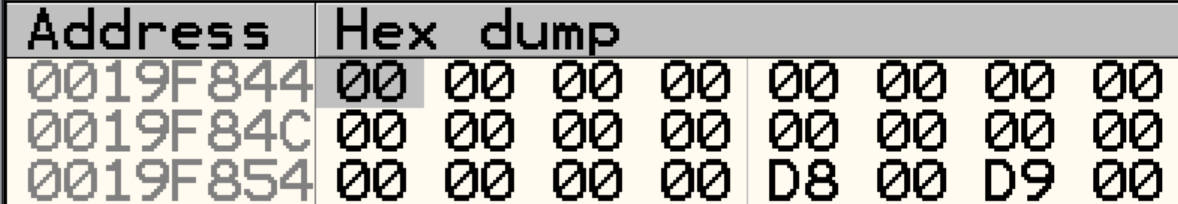
\includegraphics[width=\textwidth]{19f844_before_writing}
\end{figure}
\end{minipage}\hfill
\begin{minipage}{0.3\textwidth}
\begin{figure}[H]
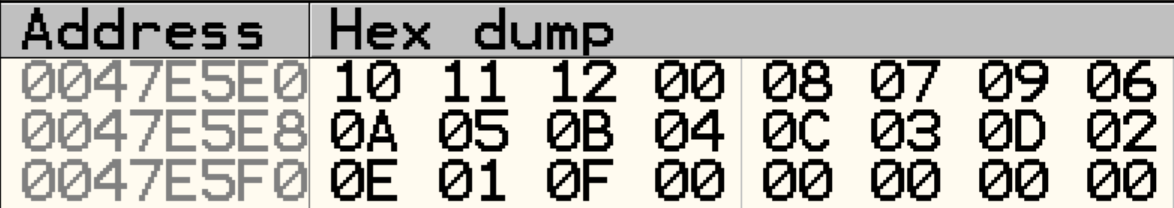
\includegraphics[width=\textwidth]{offsets_at_47e5e0}
\end{figure}
\end{minipage}\hfill
\begin{minipage}{0.3\textwidth}
\begin{figure}[H]
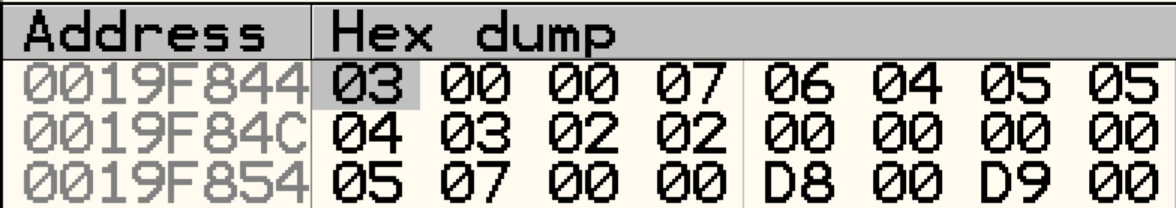
\includegraphics[width=\textwidth]{19f844_after_writing}
\end{figure}
\end{minipage}\\

\noindent
\begin{minipage}{0.3\textwidth}
Dump prima della scrittura
\end{minipage}\hfill
\begin{minipage}{0.3\textwidth}
Offsets da aggiungere a \key{19f844} per determinare l'indirizzo di scrittura
\end{minipage}\hfill
\begin{minipage}{0.3\textwidth}
Dump dopo la scrittura
\end{minipage}\\

\noindent
La funzione continua invocando \attachcode{FUN_0046d850}, con i seguenti parametri RIVEDERE: 
\begin{center}
\begin{tabular}{|c|c|}
\hline
Parametro 1, \key{ECX} & l'indirizzo \key{ECX}\\
\hline
\key{Parametro 2} & il valore \key{0x13} \\
\hline
Parametro 3 & l'indirizzo \key{19f844}\\
\hline
\key{EDX} & l'indirizzo \key{19f5e4} \\
\hline
\end{tabular}
\end{center}

In seguito, recupera il valore \key{11e} da \key{EBP - c} e il valore \key{1b} da \key{EBP - 8}: questi sono i risultati delle prime due invocazioni di \attachcode{FUN_0046db50_decode_bytes}. Questi valori vengono sommati tra loro e il risultato viene salvato in \key{EBP - 10h}. \\

Inizia ora un ciclo che inizia caricando in \key{EAX} l'indirizzo \key{19f5e4}, che dovrebbe puntare ai byte appena scritti nell'ultima invocazione. Poi invoca la funzione \attachcode{FUN_0046dc30_read_with_computed_offset}, che prende in input proprio quell'indirizzo insieme a \key{19f9b0}. Il valore di ritorno viene di fatti confrontato con i valori \key{16, 17 e 18}, ma è previsto anche un ramo \key{else}. Il confronto, però, avviene attraverso delle sottrazioni:
\begin{myverb}
CALL FUN_0046dc30_read_with_computed_offset
MOV ECX, EAX
SUB ECX, 0x10
JZ LAB_46ddd8   ; viene ritornato 16
DEC ECX
JZ LAB_46dc30   ; viene ritornato 17
DEC ECX
JZ LAB_46deec   ; viene ritornato 18
;   default_case
\end{myverb}

Nel ramo \key{default_case}, il byte meno significativo del valore ritornato viene messo nell'indirizzo ottenuto da \key{EBP + ESI - 150h}, che corrisponde a \key{19f844 + ESI}, con \esi{}. Questo ramo termina incrementando la variabile di ciclo.\\

Nel caso in cui venga restituito il valore \key{0x10}, si legge il byte scritto nella precedente iterazione e viene salvato in \key{EBP - 4} prima di invocare \attachcode{decode_bytes}. Il risultato viene controllato per verificare che sia diverso da 0, e, in questo caso, si invoca \attachcode{FUN_004021c0_write_param2_on_param1_param3_times} con questi parametri:
\begin{center}
\begin{tabular}{|c|c|c|}
\hline
\cellcolor{cellcolor}Parametro & \cellcolor{cellcolor}Valore a \textit{run time} & \cellcolor{cellcolor}Note \\
\hline
\key{Parametro 1} & \key{19f99b} & \makecell{Dove andrebbe scritto il valore \\ dell'iterazione corrente} \\
\hline
\key{Parametro 2} & \key{6} & Valore scritto nell'iterazione precedente \\
\hline
\key{Parametro 3} & \key{6} & Valore restituito da \attachcode{decode_bytes}\\
\hline
\end{tabular}
\end{center}

Nel caso in cui viene ritornato il valore \key{17}, si cambiano solo i parametri di input per la funzione \attachcode{FUN_004021c0_write_param2_on_param1_param3_times}: il secondo parametro risulta costante e pari a \key{0}.\\

Il ciclo termina dopo \key{139h} iterazioni, senza mai esplorare il ramo del caso in cui 	\attachcode{FUN_0046dc30_read_with_computed_offset} ritorni 18. \\

Al termine del ciclo, viene invocata la funzione \attachcode{FUN\_0046d850} per due volte con parametri, rispettivamente:
\paramtable[ECX;EDX;Parametro 3; Parametro 4]{FFFFFFF3 equiv -13$_{10}$;1969c4;19f844;11e}
\paramtable[ECX;EDX;Parametro 3; Parametro 4]{FFFFFFF3 equiv 286$_{10}$;19fc24;19f962;1b}


\target{FUN\_0046d850}
\subsubsection{FUN\_0046d850}
La funzione azzera 8 \key{dword} a partire dall'indirizzo contenuto in \key{EDX} prima di iniziare un ciclo in cui si legge i bytes all'indirizzo passato come parametro a \key{EBP + 8} (quindi il secondo, ma \ghidra{} lo considera come terzo parametro), con le seguenti istruzioni:
\begin{myverb}
MOV dword ptr EAX, [EBX + c]
MOVZX EAX, byte ptr [ECX + EAX]
LEA EAX, [EDX + EAX * 0x2]
INC word ptr [EAX]
INC ECX
\end{myverb}
partendo con \key{ECX = 0}. Si sta quindi accedendo ai bytes scritti prima e, dopo averli moltiplicati per due, si usano come offset per accedere a una zona di memoria di 2 bytes che viene incrementata. Tuttavia i primi 2 bytes dell'area puntata da \key{EDX} vengono successivamente azzerati. \\
Si inizia poi un altro ciclo, composto dal seguente codice:
\begin{myverb}
	loop_start:
MOVZX EBX, dword ptr [ECX]
MOV word ptr [EAX + ECX], SI
ADD ESI, EBX
ADD ECX, 0x2
DEC EDI
JNZ loop_start
\end{myverb}
Si parte con:
\begin{center}
\begin{tabular}{|c|c|}
\hline
\key{ECX} & \key{19f5e4}\\
\hline
\key{EAX} & \key{ffffffc8 = -56}$_{10}$  \\
\hline
\key{ESI} & \key{0} \\
\hline
\key{EBX} & \key{0} \\
\hline
\key{EDI} & \key{10h} \\
\hline
\end{tabular}
\end{center}
Quindi si accede alle 16 parole indicizzate da \key{19f5e4} in poi per leggerne il contenuto, sommarlo ad \key{ESI} e scriverlo in \key{EAX - 56}$_{10}$. Vengono quindi modificati i 32 bytes $\in$ [\key{19f5e4}, \key{19f604}].\\
Venono poi scritti altri byte di un'altra zona di memoria, utilizzando però sempre i byte scritti precedentemente: 
\begin{myverb}
	loop_start:
MOV EAX, dword ptr [EBP + 19f844]
CMP byte ptr [EAX + ECX], 0x0
JZ label_1
MOVZX ESI, byte ptr [EAX + ECX]
MOVZX ESI, word ptr [EBP + ESI * 2 - 0x20]
MOV word ptr [EDX + ESI * 2 + 0x20]
MOVZX EAX, byte ptr [EAX + ECX]
LEA EAX, [EBP + EAX * 2 - 0x20]
INC word ptr [EAX]
	label_1:
INC ECX
CMP ECX, dword ptr [EBP + c] ; contiene 0x13
JC loop_start
\end{myverb}
\begin{center}
\begin{tabular}{|c|c|}
\hline
\key{ECX} & \key{0}\\
\hline
\key{EAX} & \key{19f844} \\
\hline
\key{ESI} & \key{c} \\
\hline
\key{EBX} & \key{19f9b0} \\
\hline
\key{EDI} & \key{0} \\
\hline
\end{tabular}
\end{center}
Dopo queste operazioni la funzione ritorna con \key{EAX = 19f844}.


\target{FUN\_0046dc30\_read\_with\_computed\_offset}
\subsubsection{FUN\_0046dc30\_read\_with\_computed\_offset}
Questa funzione prende in input due indirizzi: quello della struttura dati e quello da usare come base per leggere il valore di ritorno. \\
Definisce al suo interno un ciclo in cui viene invocata la funzione \attachcode{FUN_0046dac0_read_following_bit} e il suo valore viene salvato in \key{ESI}, sommato al precedente contenuto moltiplicato per 2:
\begin{myverb}
CALL FUN_0046dac0_read_following_bit
LEA ESI, [EAX + ESI * 0x2]
\end{myverb}
Al valore così ottenuto viene sottratto il contenuto della \key{word} nella zona di memoria indicizzata da \key{EDI}, che contiene inizialmente \key{param_2 + 2}. Il ciclo termina solo quando il valore così ottenuto è negativo. La somma dei valori delle varie \key{dword}s viene memorizzato in \key{EBX}.\\
Alla fine del ciclo, si somma al valore negativo in \key{ESI} la somma delle varie \key{word}s lette, contenuto in \key{EBX}: si ottiene un offset da aggiungere a \key{param_2 + 0x20} per leggere il valore da restituire.

\target{FUN\_0046e340}
\subsubsection{FUN\_0046e340}
La funzione invoca \attachcode{FUN_<>_read_with_computed_offset} e confronta il valore restituito con il valore \key{0x100}. Se sono diversi, inizia un ciclo in cui, per prima cosa, si conrolla se il risultato di \attachcode{FUN_<>_read_with_computed_offset} sia maggiore al valore \key{0x100}. 

La funzione inizia un ciclo in cui viene invocata \attachcode{FUN_0046dac0_read_following_bit}. Poi c'è un ciclo:
\begin{myverb}
XOR ESI, ESI
	loop:
MOV ECX, dword ptr [EBP + 8] 	; param 1 = 19f9b0
CALL read_following_bit
ADD EDI, 0x2
LEA ESI, [EAX + ESI * 0x2]
MOVZX EAX, word ptr [EDI]
ADD EBX, EAX
SUB ESI, EAX
JNS loop
\end{myverb}
\paramtable[EAX;ECX;EDX;EBX;ESI;EDI]{19f5e4;13, cambiato in 19f9b0;19f5e4;0;0;19f5e4}


\target{FUN\_004021c0\_write\_param2\_on\_param1\_param3\_times}
\subsubsection{FUN\_004021c0\_write\_param2\_on\_param1\_param3\_times}
Riceve in input 3 parametri:
\begin{center}
\begin{tabular}{|c|c|}
\hline
\cellcolor{cellcolor}Parametro & \cellcolor{cellcolor}Valore \\
\hline
\key{Parametro 1} &  \\
\hline
\key{Parametro 2} & \\
\hline
\key{Parametro 3} & \\
\hline
\end{tabular}
\end{center}
Si confronta il parametro 3 con il parametro 1 e, se sono uguali, la funzione ritorna. Altrimenti si continua controllando il \key{byte ptr} passato come parametro 2. Se questo non è 0, c'è ancora un altro controllo: si verifica che il terzo parametro sia minore di \key{0x80 $\equiv$ 128}$_{10}$. Si ha quindi:
\begin{myverb}
if (param_3 == param_2){
   return param_1;
}
else{
   if ((byte) param_2 == 0 && param_3 >= 128 && *DAT_00484a54 != 0){
      /* mai esplorato in invocazioni da fun_46dcf0. Neanche la 
      terza condizione viene mai raggiunta in realtà */
      ...   
      return;
   }
   ...
}
\end{myverb}
Quando la tripla condizione non viene presa, si salva in \edi{} il valore di \ecx{}, poi si controlla che il terzo parametro sia minore di 4. Se non lo è, si nega \ecx{} e si mette in \key{AND} con il valore 3. Se il risultato non è 0, si sottrae al parametro 3 il valore ottenuto e si inizia un ciclo \textit{do-while} in cui si scrive nell'area puntata da \edi{} (che contiene il precedente valore di \ecx{}) il \key{byte ptr} passato come parametro 2 per un numero di volte pari al nuovo valore di \ecx{}. In seguito si calcola $\eax{} \cdot (2^8 + 1) \cdot (2^{16} + 1)$, e successivamente si salva in \ecx{} il risultato di $\frac{\text{\edx{}}}{4}$, mentre \edx{} viene messo in \key{AND} con il valore 3.
\begin{myverb}
edi = ecx;
if (param_3 >= 4){
   ecx = (~ ecx) & 3;
   if (ecx != 0){
      param_3 = param_3 - ecx;
      do {
         *edi = (byte) param_2;
         edi++;
         ecx--;
      } while (ecx != 0)  
   }
   eax = (byte) param_2 * (2^8 + 1) * (2^16 + 1); 
   // se param_2 era 6, eax diventa 06060606 
   ecx = param_3;
   param_3 = param_3 & 3;
   ecx = ecx >> 2;
}
\end{myverb}
Nel caso in cui si ottenga come risultato un valore $ n \neq 0$, si scrivono n \key{dword} in \edi{} con il valore di \eax{}. Sostanzialmente, si sta continuando a fare quello che si faceva nel ciclo \textit{do-while}, operando però 4 bytes alla volta: il valore di \eax{} infatti è del tipo \key{06060606}, supponendo che 6 sia il valore del parametro 2. Questo è giustificato dal fatto che, dato un interon, allora \code{n \% 4 == n \& 3}. Con le ultime 3 istruzione dello \textit{pseudo-codice} precedente, quindi, si è messo il resto della divisione intera tra il terzo parametro e il valore 4 in \edx{}, mentre il risultato è in \ecx{}. Essendo che ogni \key{dword} sono 4 bytes, si azzerano tante \key{dword} quante contenute in \ecx{}. Successivamente, si continua a scrivere in \edi{} un byte alla volta il valore del \key{byte ptr} del secondo parametro, per tante volte quanto il resto della divisione intera.\\
La funzione ritorna in seguito il primo parametro.\\

Riassumendo, questo ramo della funzione non fa altro che scrivere sull'indirizzo ricevuto come primo parametro il byte preso come secondo parametro per tante volte quanto specificato nel terzo parametro.


\target{FUN\_00429ea0}
\subsection{FUN\_00429ea0}
La funzione invoca subito \attachcode{FUN_00401018_set_EAX_as_SEH_handler}. Dopo vengono allocati \key{0x1f4} bytes sullo stack e si salvano alcuni registri. C'è poi un confronto tra \key{DAT_004831f8_key_and_files_virtual_alloc_address} e \key{EBX}, azzerato precedentemente. Se fossero uguali, la funzione ritornerebbe. Essendo diversi, però, continua invocando \code{SetErrorMode} con i seguenti parametri:
\paramtable[ErrorMode]{8003}
\nota{Il valore \key{8003} corrisponde alla combinazione
\code{SEM_FAILCRITICALERRORS|SEM_NOGPFAULTERRORBOX|SEM_NOOPENFILEERRORBOX}.}\\

Con questa invocazione, si previene la creazione di:
\begin{itemize}
\item \key{Critical-error-handler message box}: l'eventuale errore viene inviato al processo stesso
\item \key{Windows Error Reporting Dialog}
\item \key{Message Box} per fallimento dell'\api{} \code{OpenFile}
\end{itemize}

Successivamente viene invocata \code{SetUnhandledExceptionFilter}, con cui si imposta la \textit{default routine} per la gestione delle eccezioni come la funzione \key{FUN_41f820}. Segue un'invocazione di \attachcode{FUN_0042cf00_adjust_token}, che non riceve parametri. \\
La funzione continua mettendo in \key{EAX} l'indirizzo che contiene i dati della chiave e dei file da creare, per poi controllare se \code{byte ptr [EAX + e] == BL}, con \code{BL == 0}. In \code{[EAX + e]} è contenuto il valore \key{01}, quindi si continua invocando \code{GetSystemDefaultLangID}, che ritorna il valore \key{540410}. Dovrebbe ritornarnare un valore a 16 bit:\\
\begin{center}
\begin{tabular}{|c|c|}
\hline
SubLanguage ID & Primary Language ID\\
\hline
$bits\ \in [10, 15]$ & $bits\ \in [0, 9]$ \\
\hline
\end{tabular}
\end{center}
%+-------------------------+-------------------------+\\
%|     SubLanguage ID      |   Primary Language ID   |\\
%+-------------------------+-------------------------+\\
%15.........................10..9.............................0 bit\\

Il valore \key{0410} del registro \key{AX} rappresentano il codice \key{it-IT}, come riportanto in \href{https://winprotocoldoc.blob.core.windows.net/productionwindowsarchives/MS-LCID/\%5bMS-LCID\%5d-210407.pdf}{questo pdf scaricabile dalla documentazione microsoft}.\\
Viene controllato il valore di \key{Primary Language ID}, confrontandolo con il valore \key{0x0019}, che dovrebbe corrispondere alla sigla \key{ru}. Poiché il confronto non va a buon fine, viene invocata \code{GetUserDefaultLangID}, per ottenere lo stesso valore precedente: \key{0410}. A questo punto, dopo aver fatto gli stessi controlli sul byte meno significativo, ripete la sequenza di istruzioni: invocazione a \code{GetUserDefaultLangID}, \code{AND AX, SI}, con \key{SI = 0x3ff} e \code{CMP AX, 0x19}; segue però un \code{JNZ} che quindi viene preso. Si continua mettendo in \key{EAX} l'indirizzo che contiene la chiave RSA e i file di testo da creare, e si recupera la \key{dword} all'offset 8: \code{MOV EAX, dword ptr [EAX + 0x8]} per confrontarla col valore 0 contenuto in \key{EBX}. Il successivo \code{JBE} non viene preso, perché il valore letto è \key{0xc}. Viene eseguita una moltiplicazione con segno tra \key{EAX} e \key{3e8 = 1000}$_{10}$, e il risultato viene salvato in \key{EAX}. Viene poi messo sullo stack e usato come parametro di una invocazione di \code{Sleep}: si dorme per 12 secondi.\\
Si mette poi in \eax{} l'indirizzo ottenuto da \key{EBP - 0xac = 19fe30} per poter invocare la funzione \attachcode{FUN\_0041f680\_get\_path\_name\_struct} con i seguenti parametri:
\paramtable{19fe30;0}

Quando la funzione ritorna , si carica in \eax{} l'indirizzo di \key{EBP - 0xd0 = 19fe0c}. Questo valore viene messo sullo stack, prima di  impostare a 1 il valore 0 inserito sullo stack dall'invocazione di \code{FUN_00401018_set_EAX_as_SEH_handler}. Viene poi invocata la funzione \attachcode{FUN\_0041f560\_get\_tmp\_path\_in\_struct}.\\
Quando la funzione ritorna, si mette in \eax{} l'indirizzo che contiene il buffer con la chiave e il testo dei files, \textbf{scritto nell'altro ramo del main}. Poi si modifica il valore che la funzione \code{FUN\_00401018\_set\_EAX\_as\_SEH\_handler} aveva messo a 0 e che era stato precedentemenente aggiornato a 1, ponendolo uguale a 2.\\
Ora si controlla il 12$^o$ byte del buffer puntato da \eax{} e lo si confronta con il valore di \key{BL = 00} con \code{CMP byte ptr [EAX + 0xc], BL}. Essendo uguali, il successivo \key{JZ} viene preso. Questo salto evita l'esecuzione di gran parte del codice della funzione, che quindi non viene analizzato e porta l'esecuzione all'interno di un ciclo.\\
Si continua mettendo in \eax{} l'indirizzo di \key{EBP - 0xfc = 19fde0}, che viene messo sullo stack prima di invocare \attachcode{FUN_00431440_get_half_md5_struct}.
La funzione ritorna quindi una struttura dati \key{buffer_handler_ASCII}, col buffer contenente la prima metà dell'md5 dei byte \key{0x1e 0xfb 0x19}. Questa struttura viene copiata nella variabile globale \key{DAT_00481fb4_half_md5_struct} con la funzione \code{FUN_004203a0_copy_param_1_in_this}, e poi si invoca \code{FUN_004192f0_reset_struct} sulla struttura ritornata. \\
Segue una invocazione di \attachcode{FUN_00426a40_get_mutex_or_init_events_obj} che non riceve parametri.\\
Si controlla il valore di ritorno e, se questo è 0, si continua invocando \attachcode{FUN_004270f0_search_for_atom}. Il valore di ritorno viene confrontato con il valore 0 e, se lo è, si confronta il byte all'offset \key{0xf} della zona di memoria \key{DAT_004831f8_key_and_files_virtual_alloc_address} con il valore 0. Se sono uguali, si salta gran parte della funzione.\\
Si continua caricando in \eax{} l'indirizzo \key{19fe7c}, viene messo sullo stack prima di invocare l'immensa funzione \attachcode{FUN_00423740_generate_md5_hash_from_stack_charset}.
La funzione appena invocata restituisce una struttura contenente una stringa di 16 caratteri. Questa verrà usata come metà di una hash: infatti, il codice continua copiando la struttura appena restituita nella variabile globale a \key{DAT_00481fb4_half_md5_struct};\\
La funzione continua mettendo in \eax{} il buffer contenente testo del file e la chiave rsa, e mette sullo stack la dword all'offset \key{0x1043} e l'indirizzo dell'offset \key{0x1047}. Si mette in \ecx{} la variabile globale \key{DAT_00481fd0_rsa_struct} che sembra essere una \key{handler_buffer_ASCII} con i primi 20 bytes a 0 e il campo \key{buffer_len} impostato a \key{0xf}. Si invoca poi \attachcode{FUN_0041f9d0} con parametri:
\paramtable[ECX;EDX;Parametro 1;Parametro 2]{481fd0;21f0000;8a1047;0x114}
con l'obiettivo di copiare nella struttura dati in \ecx{} la chiave RSA specificato all'offset passato.\\
Si carica poi in \eax{} l'indirizzo all'offset \key{0x1493} del buffer \key{DAT_004831f8_key_and_files_virtual_alloc_address} che punta all'inizio del testo da inserire nel file testuale da creare; in \ecx{} viene messa \key{DAT_00481fec_txt_file_struct} e si invoca \attachcode{FUN_0041fd90_init_from_buffer_wrapper} con parametri:
\paramtable[ECX;Parametro 1]{DAT_00481fec_txt_file_struct;8a1493}
La stessa cosa viene fatta per l'offset \key{0x2493}, che punta invece al contenuto del file \key{htm} creato. La struttura dati riempita è \key{DAT_00482008_htm_file_struct}.\\

Si procede costruendo in \key{19feb8} la stringa \key{FF000000000000FF} di 16 bytes, con successivo terminatore di stringa. Con un ciclo, si calcola la lunghezza della stringa appena costruita, e la si usa come parametro della successiva \attachcode{FUN_00418ce0_find_char_in_buffer}, invocata con:
\paramtable[ECX;Parametro 1;Parametro 2;Parametro 3]{DAT_00481fec_txt_file_struct;19feb8, che punta alla stringa sullo stack;0;0x10}
Se la sottostringa viene trovata, si invoca la funzione \attachcode{FUN_0041e440} con parametri:
\begin{center}
\begin{tabular}{|c|c|}
\hline
\cellcolor{cellcolor}Parametro & \cellcolor{cellcolor}Valore \\
\hline
\key{ECX} & \makecell{\key{DAT_00481fec_txt_file_struct} }\\
\hline
\key{Parametro 1} & \makecell{\key{0x314: offset in cui è stata trovata la sottostringa} }\\
\hline
\key{Parametro 2} & \makecell{\key{0x10: lunghezza della stringa} }\\
\hline
\key{Parametro 3} & \makecell{\key{DAT_00481fb4_half_md5_struct} }\\
\hline
\key{Parametro 4} & \makecell{\key{0} }\\
\hline
\key{Parametro 5} & \makecell{\key{-1} }\\
\hline
\end{tabular}
\end{center}
Una volta sostituiti tutti gli identificativi dal file testuale, si ripete la stessa logica per il file \key{htm}.\\

Si mette sullo stack il valore \key{19fdfc} e si invoca \attachcode{FUN_0046c640}.\\

Il codice continua confrontando il byte ptr all'offset \key{0x6493} del buffer con la chiave rsa e i file con il valore 0. Essendo diversi, viene invocata \attachcode{FUN_00476b50_load_nt_funcs_and_create_thread}.\\

Vengono poi creati due thread all'interno di un loop con la funzione
\code{CreateThread}, che prendono come routine di partenza la funzione \attachcode{FUN_00429b40_thread_func}. La \textit{thread procedure} riceve un parametro di tipo \key{buffer_handler_UNICODE}, diverso per i due thread: 
\image{thread_params;0.4}
{\centering \textit{I due thread verranno riferiti rispettivamente come \key{thread 1} e \key{thread 2}}\par}
\bigskip

Gli handle restituiti vengono usati per creare una struttura dati di due campi:
\begin{center}
\begin{tabular}{|c|}
\hline
\key{thread handle}\\
\hline
\key{TID} \\
\hline
\end{tabular}
\end{center}
{\centering Struttura \key{thread_manager} \par}
\bigskip

Le strutture restituite vengono messe all'interno di \key{DAT_488204}, che sembra essere a sua volta una struttura dati fatta così:
\begin{center}
\begin{tabular}{|c|}
\hline
\key{list_start}\\
\hline
\key{list_end} \\
\hline
\key{unknown. Uguale a list_end}\\
\hline
\end{tabular}
\end{center}
{\centering Struttura \key{thread_manager_list} \par}
\bigskip

Viene poi invocata la funzione \attachcode{FUN_0040fa10}\\

Dopo una serie di invocazioni poco chiare, la funzione si mette in attesa della terminazione dei thread i cui handle sono presenti nella lista \key{thread_manager_list}: sono i thread che cifrano i files. \\

Dopo averli attesi entrambi, si continua costruendo sullo stack \key{opt321} ASCII, e si invoca \code{FUN_004273c0_add_atom_to_local_and_global_table}, al cui interno viene costruita la stringa \key{$\sim\sim\sim$<hash_id>$\sim\sim\sim$} e la si usa come parametro di \code{AddAtomA} e \code{AddGlobalAtomA}: viene registrata l'hash descrittiva dell'utente anche all'interno della atom table di sistema. \\

Poi si accede a \key{DAT_00481ffc} e se è diversa da 0 si invoca \attachcode{FUN_00425870_create_desktop_files_and_open_them}.
La funzione, infine, invoca 	\attachcode{FUN_00431de0}


\target{FUN\_00431de0}
\section{FUN\_00431de0}
La funzione recupera in una struttura UNICODE il path completo dell'eseguibile e genera un'altra struttura UNICODE contente il path della cartella \key{Temp}. Dopodiché, si invoca \code{SetFileAttributesW} sulla prima struttura, impostando i \key{FileAttributes = NORMAL}: il file non avrà altri attributi.\\
Si confrontano poi i path delle due strutture e, se sono diversi, si costruisce sullo stack la stringa \key{sys} e si invoca \code{FUN_0042f4b0_gen_tmp_file_and_get_its_name_in_UNICODE_struct}, che genera il nome di un file temporaneo a partire da un path e prefisso passati e, se il nome generato è unico, viene creato un file vuoto con quel nome e viene restituito un handle a quel file. Qui si passa come path quello della cartella \key{Temp}, e come prefisso \key{sys}; l'handle restituita non viene presa in considerazione.\\
Si invoca poi la funzione \code{MoveFileExW} per \textit{spostare} l'eseguibile nel nuovo file temporaneo creato. Il parametro \key{dwFlags} di questa invocazione è \key{0x9 = 1 | 8 = MOVEFILE_REPLACE_EXISTING | MOVEFILE_WRITE_THROUGH}: il primo specifica che, se la destinazione è il nome di un file esistente, il suo contenuto viene sovrascritto con il contenuto di quello vecchio. Il secondo flag, invece, specifica che la funzione non ritorna finché lo spostamento non è effettivamente avvenuto. C'è poi una seconda invocazione di \code{MoveFileExW} con parametri: 
\paramtable[lpExistingFileName;lpNewFileName;dwFlags]{<path_al_file_temporaneo>;0;0x4 = MOVEFILE_DELAY_UNTIL_REBOOT} 
Con questa configurazione degli ultimi due parametri, si contrassegna il file esistente come un file da eliminare al prossimo riavvio del sistema.\\
Infine, si costruisce sullo stack la stringa \key{cmd.exe /C del /Q /F "}; a questa viene concatenato il nome del file temporaneo seguito da \key{"} e viene usata per la costruzione di una struttura UNICODE. Questa struttura viene quindi passata a \code{FUN_0042ec10_run_given_command} prima di terminare l'esecuzione con una invocazione di \code{ExitProcess}.




\target{FUN\_00425870\_create\_desktop\_files\_and\_open\_them}
\section{FUN\_00425870\_create\_desktop\_files\_and\_open\_them}
Si imposta un anello della catena.\\
Poi si procede invocando \code{FUN_00420a70_get_struct_of_dir_by_CSIDL}, specificando come terzo parametri il \key{CIDL CSIDL_DESKTOPDIRECTORY = 0x10}: si sta recuperando nel buffer passato come primo parametro una struttura UNICODE che conterrà il path al desktop. Questa struttura è usata come base per altre strutture UNICODE, che contengono nel loro buffer le seguenti stringhe UNICODE:
\begin{enumerate}
\item \key{<desktop_path>\tbs{}asasin.htm}
\item \key{<desktop_path>\tbs{}asasin.bmp}
\end{enumerate}
La prima struttura viene passata in input a \code{FUN_0042e6b0_file_exist}, che ritorna 1 se il file esiste, 0 altrimenti. Se il file non esiste, viene quindi invocata \code{FUN_0042e7d0_create_asasin_file} passando gli opportuni parametri; si sta creando il file \key{.htm} sul desktop. \\
Si continua cercando l'esistenza del file relativo alla seconda struttura e, se non c'è, si crea una struttura con il contenuto del file testuale e la si passa come primo parametro della funzione \attachcode{FUN_004248b0_get_bitmap_bytes_in_ASCII_struct}, insieme a un parametro di output che conterrà una satruttura ASCII contenente i bytes della bitmap. Questa struttura viene poi passata a \code{FUN_0042e7d0_create_asasin_file} insieme alla struttura che contiene il path completo del file bitmap affinché questo possa essere creato.\\
Si continua costruendo sullo stack la stringa ASCII \key{Control Pane\tbs{}Desktop} e la si usa come parametro \key{subkey} per la successiva invocazione di \code{FUN_00416290_RegOpenKeyExA_wrapper}: si sta recuperando l'handle a questa chiave di sistema con accesso \key{KEY_QUERY_VALUE | KEY_SET_VALUE}, in modo da poter cambiare lo sfondo del desktop. Infatti, si costruisce ancora sullo stack la stringa \key{WallpaperStyle} e si invoca \code{FUN_004205a0_add_REG_SZ_type_value}, che ha come obiettivo quello di aggiungere un valore di tipo \key{REG_SZ} alla chiave la cui handle è passata in \ecx{}, precedentemente aperta. Si imposta quindi il valore \key{WallpaperStyle = "0"} della chiave di sistema \key{Control Pane\tbs{}Desktop}. \\
Si continua poi cambiando un altro valore: \key{TileWallpaper}, con valore \key{0}: in questo modo, come riportato nella \href{https://docs.microsoft.com/it-it/windows/win32/controls/themesfileformat-overview#control-paneldesktop-section}{documentazione}, l'immagine risulterà centrata. Si invoca poi la funzione \code{SystemParametersInfoW}, che consente di impostare il valore di un parametro di sistema. I parametri che riceve sono:
\paramtable[Action;wParam;lParam;UpdateProfile]{SPI_SETDESKWALLPAPER;0;<path_dell'immagine_bitmap_sul_desktop>;3}
Questa invocazione imposta effettivamente l'immagine come sfondo.\\
Si continua poi invocando la funzione \code{ShellExecuteW}, con comando \key{"open"} sia sul file \key{.htm} che quello \key{.bmp}.\\
Infine, la funzione ritorna rilasciando le risorse ancora allocate.




\target{FUN\_004248b0\_get\_bitmap\_bytes\_in\_ASCII\_struct}
\section{FUN\_004248b0\_get\_bitmap\_bytes\_in\_ASCII\_struct}
Viene impostato un anello SEH.\\
Poi si invoca la funzione \code{FUN_00416c60_store_DC_handle_in_this} per recuperare un \textit{device context} all'intero schermo. Questa handle viene poi passata come parametro per la successiva \code{FUN_00416dc0_CreateCompatibleDC_wrapper}, che crea invece un \textit{memory device context} compatibile con il device specificato. L'handle restituita da questa invocazione viene invece passata a \code{GetDeviceCaps}, con parametro \key{index = LOGPIXELSY}: si stanno recuperando il numero di pixel per pollice logico sull'asse verticale dello schermo. Questo valore, \key{0x60} nel mio caso, viene passato a \code{MulDiv} per calcolare:
\[ 	\frac{\key{0x60} \cdot \key{0x12}}{\key{0x48}}	\]
Viene poi invocata la funzione \code{CreateFontA}, che riceve in input i seguenti parametri:
\image{CreateFontA_params;0.4}
Si continua invocando \code{FUN_00416e30_replace_object_in_DC}, che rimpiazza nel \key{DC} passato in \ecx{} l'oggetto dello stesso tipo di quello passato come parametro 1; in questo caso si sta sostituendo il font con quello appena creato.\\
Si invoca poi \code{FUN_00416fc0_DrawText_wrapper} per scrivere il testo del messaggio. Il valore di ritorno non viene considerato e viene subito sovrascritto. \\
Si invoca poi \code{FUN_004189e0_create_compatible_bitmap_wrapper} che crea una bitmap compatibile con il device associato al DC passato. L'handle alla bitmap creata viene poi passata a \code{FUN_00416e30_replace_object_in_DC} per sostituirla nel DC.\\
Si invoca \code{CreateSolidBrush} con parametro \key{0x404040} \textcolor[HTML]{404040}{\rule{0.3cm}{0.3cm}} per ottenere un identificativo a un \textit{brush} logico.\\
Si invoca \code{FUN_00417220_FillRect_wrapper} su un'altra struttura dati \key{RECT}, alla posizione \key{199fae4}, con il colore appena costruito. Successivamente, sempre sull'handle al colore, si invoca \code{DeleteObject} per liberarne le risorse e rilasciare l'handle.\\
Si invoca poi \code{FUN_004170a0_SetTextColor_wrapper} con colore \key{0xff8080} \textcolor[HTML]{ff8080}{\rule{0.3cm}{0.3cm}}.\\
Si invoca poi \code{SetBkMode_wrapper} per impostare la \textit{background mode} del DC passato. In questo caso viene impostata a \key{0x1 = TRANSPARENT}: il background rimane \textit{untouched}.\\
Si ripetono poi le operazioni di \code{FUN_00416fc0_DrawText_wrapper}, \code{CreateSolidBrush}, questa volta con parametro \key{0x00ff00} \textcolor[HTML]{00ff00}{\rule{0.3cm}{0.3cm}}, per poi invocare \code{FUN_004172e0_FrameRect_wrapper}: si sta disegnando la cornice verde.\\
Si procede invocando \code{FUN_004168e0_GetObjectA_wrapper}, per recuperare \key{0x18} bytes di informazioni sulla bitmap.\\
Si procede poi a calcolare una dimensione in byte che probabilmente rappresenta la dimensione dell'immagine, e si inizializza una struttura con la funzione \attachcode{FUN_0041e310_get_empty_ASCII_struct_of_given_size}. Si procede scrivendo \textit{hardcoded} nei primi bytes di questo buffer quello che sarà l'header dell'immagine bitmap e poi si invoca \code{FUN_00416ee0_GetDIBits_wrapper} per ricevere i bit di una bitmap e salvarli in un apposito buffer; questo buffer non è altro che un opportuno offset del buffer allocato precedentemente.\\
La struttura dati completamente scritta viene quindi copiata in un altro indirizzo che viene ritornato dopo aver rilasciato gli handle nella struttura. 




\target{FUN\_00429b40\_thread\_func}
\section{FUN\_00429b40\_thread\_func}
Si invoca \key{set_EAX_AS_...} con parametro \key{LAB_00429e85}. Viene poi invocata \code{GetCurrentThread} per recuperare uno pseudo-handler al thread. Questo pseudo handler viene usato come primo parametro di \code{SetThreadPriority}, insieme al valore \key{-2} che corrisponde a \key{THREAD_PRIORITY_LOWEST}. \\
Si mette in \esi{} il valore del parametro e, nel caso del \key{thread 2}, si continua impostando la priorità \key{THREAD_MODE_BACKGROUND_BEGIN} per il thread corrente, facendolo eseguire in background. \\
Nel caso del \key{thread 1}, invece, verifica che il primo byte del buffer sia \key{0x63}, corrispondende al carattere \key{c}$_ASCII$. In caso di esito positivo, continua ad eseguire in \textit{foreground} e invoca \attachcode{FUN_0046bf70_get_user_file} con paramtri:
\paramtable{219ff4c, area di memoria vuota;21f13c8, buffer_handler_ASCII passata al thread 1}.
\bigskip

\nota{da qui in poi i due thread continueranno quindi a eseguire con due priorità diverse: \key{thread 1} continuerà con \key{THREAD_PRIORITY_LOWEST}, mentre \key{thread 2} con \key{THREAD_MODE_BACKGROUND_BEGIN}. Se il primo byte del \key{thread 1} non fosse stato \key{0x63}, anche questo thread avrebbe acquisito la priorità \key{THREAD_MODE_BACKGROUND_BEGIN}.}\\

L'invocazione precedente ritorna un struttura \key{file_list_manager} contenente tutti i path ai file da cifrare, che sono solo quelli i cui path iniziano con \key{C:\tbs{}Users\tbs{}<user_name>}.\\

\nota{in realtà, c'è anche un file che non \textit{match-a} il pattern: \key{c:\tbs{}ProgramData\tbs{}Microsoft\tbs{}Windows Defender\tbs{}Scans\tbs{}mpcache-A82FFA3655F96AB434E955F9850654A7BB1862BF.bin}, ma sembra essere l'unico}\\

Viene poi invocata la funzione \attachcode{FUN_00427ac0} passando come parametri la struttura dati base del thread e la struttura \key{file_list_manager} appena recuperata.


\target{FUN\_00427ac0}
\section{FUN\_00427ac0}
Viene invocata \key{set_EAX...} con parametro \key{4297ab}.\\

Viene confrontato il valore della variabile \key{DAT_481fe4}, che contiene il valore \key{0x11f}, con il valore \key{0x10}: RICERCARE COSA È.\\

La funzione recupera in \eax{} il dato \key{DAT_00481fd0_rsa_struct} e metto sullo stack \key{DAT_00481fb4_half_md5_struct}, insieme al valore in \key{DAT_00481fe0}, \key{0x114}, all'indirizzo \key{0x21f11b0} per poi invocare la funzione \attachcode{FUN_0041a310_init_crypto_weapons_struct}.

Si continua resettando a mano una \key{buffer_handler_UNICODE}  all'indirizzo \key{22bfe98}. Si mette in \ecx{} l'indirizzo \key{22bfeb4 -> 022bff4c} e si invoca \code{FUN_0041b4a0_get_24_bytes_buffer}. \\

\nota{il buffer restituito dall'invocazione di malloc viene posto all'offset 4 della struttura in \ecx{}. Si nota che il primo campo è un puntatore alla lista dei nomi dei file.}\\

Si inizia poi un ciclo, in cui si accede alla lista dei nomi per recuperare le varie struct. Ad ogni iterazione, si mette in \ecx{} la struttura \key{crypto_weapons_struct}, mentre sullo stack vengono messe la nuova struttura relativa ai file e la stringa \key{asasin}: questa è l'estensione con cui vengono memorizzati sul disco i file cifrati. Si procede poi a invocare \attachcode{FUN_00413be0_crypt_file}.\\

Quando la funzione ritorna, si contano il numero di caratteri \code{\tbs{}} nel path completo del file originale con la funzione \code{FUN_00418500_count_char_occurences}. Viene poi invocata \code{FUN_00418590_count_char_occurences} sulla struttura base del thread.\\

\nota{le funzioni hanno offset diversi, ma fanno la stessa cosa: probabilmente sono metodi di classi diverse.}\\

Si continua generando una struttura contenente il path completo della cartella parent del file in esame, per poi concatenarle ad altre strutture generate successivamente in modo da costruirne un'altra che memorizzi nel buffer la stringa formata dalla concatenazione di: \key{<path_alla_cartella_parent_del_file_cifrato>\tbs{}asasin-<4_caratteri_truly_random>.htm}.\\
Viene poi invocata \code{FUN_0042e7d0_create_asasin_file} che crea un file col nome specificato nella struttura passata come parametro 1 e scrive il contenuto passato dalla struttura ASCII passata come parametro 2. \\
Vengono poi rilasciate le risorse e si procede con un nuovo file.\\

Alla fine del ciclo, si costruiscono sullo stack delle stringhe:
\begin{itemize}
\item \key{id=}, all'indirizzo \key{EBP + 0xc}
\item \key{\&act=stats}, all'indirizzo \key{EBP - 0x20}
\item \key{\&path=}, all'indirizzo \key{EBP - 0x38}
\item \key{\&encrypted=}, all'indirizzo \key{EBP - 0x54}
\item \key{\&failed=}, all'indirizzo \key{EBP - 0x48}
\item \key{\&lenght=}, all'indirizzo \key{EBP - 0x30}
\end{itemize}

Continua poi recuperando delle strutture ASCII relative a valori numerici: calcola una struttura contenente il numero \key{22}, un'altra contenente il numero \key{0} e un'altra contenente il numero \key{2}.\\

\nota{sto seguendo il thread sulla sharedDirectory, che aveva al suo interno due files: \begin{itemize}
\item \key{ciao.txt}: il cui contenuto era \key{ciaociaociaociao}
\item \key{ciao2.txt}: il cui contenuto era \key{ciao}
\end{itemize} 
Quindi la prima struttura potrebbe essere relativa ai byte cifrati (16 + 4 + 2 terminatori) e la terza relativa al numero di file cifrati.
}\\

Genera poi un'altra struttura ASCII il cui buffer è la versione ASCII del buffer della struttura dati come parametro al thread, quindi il path al volume in esame. A partire da questa struttura ne viene creata un'altra sostituendo tutti i \key{\tbs{}} con \key{\%5C}, grazie alla funzione \code{FUN_00430f50_strsub_\_\%5c}.\\

Tutte queste informazioni vengono poi combinate per generare una struttura ASCII che memorizza:
\key{id=<half_md5>\&act=stats\&path=<volume_base_path>\&encrypted=<num_encrypted_file>\&failed=<num_failed_files>\&length=<total_encrypted_bytes>}



\target{FUN\_00413be0\_crypt\_file}
\section{FUN\_00413be0\_crypt\_file}
La funzione riceve in input 3 parametri:
\begin{center}
\begin{tabular}{|c|c|}
\hline
\cellcolor{cellcolor}Parametro & \cellcolor{cellcolor}Valore \\
\hline
\key{ECX} & \makecell{la strutura dati \key{crypto_weapons_struct}}\\
\hline
\key{Parametro 1} & \makecell{L'indirizzo della \key{buffer_handler_UNICODE} relativa al file da cifrare}\\
\hline
\key{Parametro 2} & \makecell{la stringa costante \key{asasin}}\\
\hline
\end{tabular}
\end{center}
La funzione azzera i \key{0x344} bytes a partire dall'offset \key{0x022bf6b0}. Si scrivono poi, in questa zona, 3 dwords costanti a offset differenti. \\
Si continua poi mettendo in \edi{} il campo \key{hash} della srtuttura \key{crypto_weapons_struct}; questa hash viene poi copiata sempre all'interno di questa zona di memoria azzerata, all'indirizzo \key{22bf6b4}.\\ %414789
Si invoca poi la funzione \code{FUN_0042f5c0_get_last_path_token_in_new_struct}, che prende come primo parametro una \key{buffer_handler_UNICODE} vuota, chie viene inizializzata opportunamente inserendo nel buffer il nome del file, senza il suo path: si recupera quindi solo \key{nome.estensione}. Questo viene poi copiato all'indirizzo \key{22bf7c8} tramite una \key{_memcpy}.\\
Si invoca poi la funzione \code{GetFileAttributesExW}, passandogli come buffer output l'indirizzo \key{22bf9d0}, che fa parte sempre della zona di memoria inizializzata all'inizio. L'invocazione di \code{FUN_0040f410_get_unicode_struct_from_ascii_string} costruisce in \ecx{} una struttura dati \key{buffer_handler_UNICODE} a partire da una stringa ASCII passata come parametro; in questo caso la stringa è \key{0123456789abcdef}, cioè l'insieme delle cifre esadecimali e la struttura dati è messa in \key{0x22bfbec}. L'operazione è ripetuta per creare un'altra struttura all'indirizzo \key{0x22bfc44}.\\
Il codice continua invocando \code{FUN_00412ca0_gen_truly_random_hex_string_of_specified_size} che genera una struct \key{buffer_handler_UNICODE} con buffer random della dimensione specificata come terzo parametro; l'indirizzo della struttura di output viene specificato come primo parametro, mentre il secondo parametro è la struttura con il buffer contenente la versione \key{char} dei valori esadecimali. Vengono, grazie a questa funzione, create due strutture dati con buffer di caratteri UNICODE truly random, una di 12 caratteri e l'altra di 8.\\
Si procede invocando \code{FUN_00430450_generate_UNICODE_struct_from_string} che genera nel primo parametro una struttura \key{buffer_handler_UNICODE} contenente i \key{param_3} caratteri contenuti nel buffer ASCII ottenuto come parametro 2; viene operata una conversione per ogni carattere ASCII. Con questa funzione, vengono create diverse strutture:
\begin{enumerate}
\item una contenente gli ultimi 4 caratteri della md5 half: \key{55MZ}
\item una contenente i penultimi 4 caratteri della md5 half: \key{65W0}
\item una contenente i primi 8 caratteri della md5 half: \key{BIDM66TH}
\end{enumerate}
Queste strutture sono usate per generare una nuova struttura, che conterrà nel buffer la stringa: \key{BIDM66TH-65W0-55MZ}: è praticamente l'originale, \textit{tokenizzata} da un trattino. Non è finita: si concatena questa struttura a quelle ottenute randomicamente, concatenando prima quella di 8 caratteri e poi quella di 12. Nel caso running in esame, si ottiene una struttura il cui buffer è \key{BIDM66TH-65W0-55MZ-7BCE3956-8B5BC080DC45}. Infine, si concatena questo buffer appendendo \key{.asasin}: si sta generando il nome del file cifrato in modo semi-randomico (i primi 3 token sono sempre uguali).\\
Si continua recuperando il path completo alla directory parent del file da cifrare con \code{FUN_0042f660_get_curr_file_parent_dir_full_path}, con il \key{\tbs{}} finale. Questa struttura, combinata a quella precedente, permettono la creazione di una nuova \key{buffer_handler_UNICODE} che contiene nel buffer il path completo del nuovo file cifrato.\\
Si continua recuperando un puntatore a un \textit{handle} al file esistente, aprendolo. \\
Viene poi invocata la funzione \code{MoveFileExW} con questi parametri:
\begin{center}
\begin{tabular}{|c|c|}
\hline
\cellcolor{cellcolor}Parametro & \cellcolor{cellcolor}Valore \\
\hline
\key{[in] LPCWSTR lpExistingFileName} & \makecell{\key{nome del file reale} }\\
\hline
\key{[in, optional] LPCWSTR lpNewFileName} & \makecell{\key{nome del nuovo file cifrato} }\\
\hline
\key{[in] DWORD dwFlags} & \makecell{\key{0x9} }\\
\hline
\end{tabular}
\end{center}


\nota{il valore del flag è la concatenazione di \key{MOVEFILE_WRITE_THROUGH (0x8) | MOVEFILE_REPLACE_EXISTING (1)}: il primo rende l'invocazione bloccante finché i cambiamenti non vengono \textit{flushati} sul disco, il secondo permette di sovrascrivere il contenuto del nuovo file con quello del file esistente, nel caso il nuovo file esista già.}\\

Il file viene quindi rinonimato usando la stringa costruita in precedenza, con estensione \key{.asasin}. \\
Si procede generando 16 bytes random invocando \code{FUN_00410d90_CryptoGenRandom_wrapper}, che vengono salvati in \key{22bf6c4}, campo \key{truly_random_bytes} della struttura costruita sullo stack.\\

Si invoca poi la funzione \code{FUN_0046FDF0}, che restituisce in \key{0x22bf590} dei bytes generati pseudo randomicamente (???).\\

Si invoca poi \code{FUN_00410fe0_encrypt_random_key}, per cifrare la chiave random di 16 bytes contenuta nel campo \key{truly_random_bytes(_encrypted)} della struttura \key{struct_in_crypto_func}, usando il CSP del primo campo della struttura \key{crypto_weapons}.\\

Si continua poi invocando \code{FUN_00473830_BOH} e la funzione \code{FUN_004129d0_sembra_malloc}.\\

Si invoca poi \code{FUN_004106e0_read_file_in_buffer}, per leggere il contenuto del buffer. Dopodiché questo contenuto viene cifrato invocando \code{RIVEDI NOME E ANALIZZALA}. Infine, si prosegue azzerando il \key{file_seek_pointer} e sovrascrivendo i dati con le due apposite funzioni.\\
Alla fine, viene scritto alla fine del file anche la struttura \key{struct_crypto_in_func}: è necessaria per riprendere la chiave in caso di decifratura.\\
Si invoca poi \code{GetSystemTimeAsFileTime}, valore che viene usato per impostare la data di creazione, di ultimo accesso e di ultima scrittura del file appena cifrato invocando \code{FUN_00410ad0_set_file_time_wrapper}.\\
Si continua invocando \code{FUN_004108b0_FlushFileBuffers_wrapper} per forzare la scrittura sul file di tutti i buffer e si chiude l'handle al file e rilascia tutte le altre risorse.



\target{FUN\_0046f220\_AESNI\_istructions\_supported}
\section{FUN\_0046f220\_AESNI\_istructions\_supported}
Invoca CPUID con \eax{} impostato a 1: recupera informazioni sul processore. In particolare, la funzione è interessata al 26$^{th}$ bit del registro \ecx{}: si vuole verificare se il processore supporta le instruzioni \key{AES-NI}, cioè delle istruzioni ottimizzate per la cifratura con \key{AES}.


\target{FUN\_0041a310\_init\_crypto\_weapons\_struct}
\section{FUN\_0041a310\_init\_crypto\_weapons\_struct}
La funzione riceve 4 parametri:
\paramtable[ECX;Parametro 1;Parametro 2;Parametro  3]{undefined;DAT_00481fd0_rsa_struct;[DAT_00481fe0_key_blob_len] = 0x114, lunghezza del parametro precedente;buffer_handler_ASCII contenente DAT_00481fb4_half_md5_struct}

La funzione azzera i primi 8 byte in \ecx{} e poi invoca \attachcode{FUN_00416570_get_CSP} con parametri 
\paramtable[this;Parametro 1;Parametro 2]{il valore in ECX: 0x22bfc8c;PROV_RSA_AES;CRYPT_VERIFYCONTEXT}
L'handle al \key{CSP} ottenuto viene messo sullo stack, mentre in \ecx{} viene ripristinato il valore originale per invocare la funzione \attachcode{FUN_00410cf0_put_param_1_handle_in_this}.\\

Si continua poi invocando \attachcode{FUN_00416680_get_hcryptkey} con parametri:
\paramtable[ECX;Parametro 1;Parametro 2;Parametro 3;Parametro 4]{0x22bfe48: indirizzo della struttura crypto_weapons_struct da inizializzare;[DAT_00481fd0_rsa_struct] = 0x21f11b0;0x114: lunghezza della struttura precedente;DAT_00481fb4_half_md5_struct}
Se la funzione ha avuto successo, si continua scrivendo il buffer della struttura \key{DAT_00481fb4_half_md5_struct} nel terzo campo della struttura \key{crypto_weapons_struct}, che viene poi ritornata.


\target{FUN\_00416680\_get\_hcryptkey}
\section{FUN\_00416680\_get\_hcryptkey}
La funzione invoca \code{CryptImportKey} con parametri:
\begin{center}
\begin{tabular}{|c|c|}
\hline
\cellcolor{cellcolor}Parametro & \cellcolor{cellcolor}Valore \\
\hline
\key{[in] HCRYPTPROV hProv} & \makecell{\key{handle al CSP recuperato prima} }\\
\hline
\key{[in] const BYTE *pbData} & \makecell{\key{[DAT_00481fd0_rsa_struct] = 0x21f11b0} }\\
\hline
\key{[in] DWORD dwDataLen} & \makecell{\key{0x114: lunghezza del parametro precedente in bytes} }\\
\hline
\key{[in] HCRYPTKEY hPubKey} & \makecell{\key{0: la chiave passata non è cifrata} }\\
\hline
\key{[in] DWORD dwFlags} & \makecell{\key{0: la chiave passata non è cifrata} }\\
\hline
\key{[out] HCRYPTKEY *phKey} & \makecell{0x22bfe4c: secondo campo della struttura }\\
\hline
\end{tabular}
\end{center}
L'handle restituito viene messo nell'apposito campo della struttura di tipo \key{crypto_weapons_struct}. Il risultato dell'invocazione viene anche restituito.



\target{FUN\_00410cf0\_put\_param\_1\_handle\_in\_this}
\section{FUN\_00410cf0\_put\_param\_1\_handle\_in\_this}
La funzione prende in input il \key{HCRYPTPROV} restituito dall'invocazione di \code{CryptAcquireContextA}, lo dereferenzia ottenendo l'\textit{handle} al CSP costruito e salva questo handle nell'indirizzo passato in \ecx{}. 



\target{FUN\_0046bf70\_get\_user\_file}
\section{FUN\_0046bf70\_get\_user\_file}
Riceve in input 2 parametri, che sono un'area di memoria vuota e una \key{buffer_handler_UNICODE}.\\

Si invoca \key{set_EAX_AS_...} con parametro \key{LAB_0046c12b}. \\
Poi si invoca \attachcode{FUN\_0046b310\_get\_file\_to\_crypt} con gli stessi parametri che la funzione riceve:
\paramtable{22bff08, area di memoria vuota;21f13c8, buffer_handler_UNICODE passata al thread 1}.

La funzione ritorna il valore 1, ma costruisce nel primo parametro una struttura fatta nel seguente modo:
\begin{center}
\begin{tabular}{|c|c|}
\hline
\multicolumn{2}{|c|}{\cellcolor{cellcolor}\key{file_list_manager}}\\
\hline
\cellcolor{cellcolor}Campo & \cellcolor{cellcolor}Valore \\
\hline
\key{list_start} & \makecell{Indirizzo della lista di strutture dati \key{hidden}.\\Il primo campo di ognuna di queste è una \key{buffer_handler_UNICODE}\\che contiene il nome di un file da criptare}\\
\hline
\key{list_end} & \makecell{Indirizzo in cui aggiungere il prossimo elemento.}\\
\hline
\key{end_of_allocated_space} & \makecell{Indirizzo finale della lista. }\\
\hline
\end{tabular}
\end{center}
La funzione continua poi invocando \attachcode{FUN\_0046bf00\_filter\_users\_files}, passandogli come parametro:
\begin{center}
\begin{tabular}{|c|c|}
\hline
\cellcolor{cellcolor}Parametro & \cellcolor{cellcolor}Valore \\
\hline
\key{Parametro 1} & \makecell{puntatore all'inizio della lista\\(campo 1 della struttura precedente)}\\
\hline
\key{Parametro 2} & \makecell{puntatore alla fine della lista\\(campo 2 della struttura precedente)}\\
\hline
\key{Parametro 3} & \makecell{zona di memoria vuota. Da come viene successivamente ripristinata\\sembra essere una struttura dati \key{file_list_manager}}\\
\hline
\end{tabular}
\end{center}
Viene poi invocata la funzione \attachcode{FUN_0046ac50_copy_param_1_in_this} per copiare la \key{file_list_manager} costruita precedentemente all'interno di quella zona di memoria vuota; quella originale viene invece disallocata, ma viene comunque invocata la funzione \code{FUN_00429a70_reset_file_list_manager} sulla lista disallocata.\\

La funzione ritorna quindi la strutta \key{file_list_manager} contenente tutte le struct \key{buffer_handler_UNICODE} relative ai files nel path \key{C:\tbs{}Users\tbs{}<user_name>\tbs{}}.



\target{FUN\_0046bf00\_filter\_users\_files}
\section{FUN\_0046bf00\_filter\_users\_files}
Non è stata approfondita, ma sembra rimuovere dalla lista tutti gli elementi che non iniziano con \key{C:\tbs{}users\tbs{}luca}. La cosa potrebbe ha un riscontro: provando a creare un file con estensione \key{txt} nella directory \key{C:\tbs{}}, questo non viene cifrato.


\target{FUN\_0046b310\_get\_file\_to\_crypt}
\section{FUN\_0046b310\_get\_file\_to\_crypt}
Si costruisce sullo stack la stringa \key{\tbs{}*} e la si concatena con la stringa nel buffer della struttura dati ricevuta in input. Viene passato anche il parametro di oputput, che sarà una \key{buffer_handler_	UNICODE}. \\
Viene poi invocata la funzione \code{FindFirstFileW}, passando come path in cui cercare la stringa appena costruita. La funzione restituisce un handle da usare per invocazioni successive della funzione: è probabile che si faranno chiamate successive per recuperare tutti i file dalla directory root. Il parametro di output è l'indirizzo \key{0x21bfc10} mentre l'handle restituita viene salvata in \key{21bfe60}.\\
Si invoca poi \attachcode{FUN_0040b940_reset_UNICODE_struct} sulla struttura costruita precedentemente, con il buffer \key{c:\tbs{}*}.\\
Si procede mettendo in \eax{} l'indirizzo della struttura dati ricevuta in input, mettendo sullo stack il valore \key{40000000} e invocando la funzione \attachcode{FUN_00462b10_check_access_right_on_volume}. \\
La funzione salva l'esito del controllo sullo stack e carica in \ecx{} il puntatore di tipo \key{LPWIN32_FIND_DATAW} relativa al primo file, recuperato precedentemente. Viene poi messo sullo stack l'indirizzo della struttura dati relativa al thread, prima di invocare \attachcode{FUN_0043c0f0}.\\
Se la funzione ritorna 0, verifica se il campo \key{dwFileAttributes} della struttura dati \key{_WIN32_FIND_DATAW} relativa al file in esame è \key{0x1600 = 0x1000 | 0x400 | 0x200 = FILE_ATTRIBUTE_OFFLINE | FILE_ATTRIBUTE_REPARSE_POINT | FILE_ATTRIBUTE_SPARSE_FILE}. Se il risultato dell'\key{AND} tra questi valori è 0, quindi non c'è alcun match, allora il \code{JNZ} non viene preso e si continua facendo vari controlli sempre sullo stesso campo. In particolare, se è una directory, si invoca la funzione \attachcode{FUN_0043c160_check_dir_name} con due parametri: il nome del file nel relativo campo della struttura e il valore 0.  \\
Se questa funzione ritorna il valore 0, si procede a recuperare i dati del prossimo file, altrimenti si continua verificando ancora una volta se si tratta di una directory, controllando il campo \key{dwFileAttributes}. 
\begin{itemize}
\item
Se è una directory, si invoca la funzione \attachcode{FUN_00420e10_init_UNICODE_struct_from_string_and_char}, passandogli come parametri:
\begin{center}
\begin{tabular}{|c|c|}
\hline
\cellcolor{cellcolor}Parametro & \cellcolor{cellcolor}Valore \\
\hline
\key{output struct pointer} & \makecell{\key{zona di memoria a 0, conterrà la struttura di output} }\\
\hline
\key{base string} & \makecell{\key{il path del buffer della struttura passata al thread} }\\
\hline
\key{to append char} & \makecell{\key{il carattere da appendere alla stringa \tbs{}} }\\
\hline
\end{tabular}
\end{center}
Successivamente, si invoca \code{FUN_0040f9b0_init_struct_from_2_strings} per aggiungere il nome della directory in esame al buffer ottenuto precedentemente: in questo flusso di esecuzione, si ottiene quindi una struttura dati \key{buffer_handler_UNICODE} il cui buffer è allocato con malloc e contiene \key{c:\tbs{}\$WinREAgent}. Questa struttura dati appena costruita viene passata come parametro a una invocazione ricorsiva di questa funzione: si cercano tutti i file all'interno della cartella ottenuta e delle sue sottocartelle.\\
Quando l'invocazione ricorsiva ritorna, si invoca \code{FUN_0040b940_reset_UNICODE_struct} per liberare la memoria allocata precedentemente per le due struttura dati, prima di ripartire con un nuovo file con l'invocazione di \code{FindNextFileW}.

\item Se non è una directory, invoca la funzione \code{non riesco a visualizzarla}, per verificare se il nome o il formato è all'interno di una lista costruita sullo stack byte per byte. Se la funzione non ritorna 0, quindi probabilmente non è nella lista dei nomi, si continua creando una struttura con il path completo al file in esame e lo si passa alla funzione \attachcode{FUN_0040f920_copy_UNICODE_struct_in_this_param} insieme a un altro indirizzo:
\paramtable{undefined - [ECX]; struttura dati col path completo} 
\end{itemize}






\target{FUN\_00420e10\_init\_UNICODE\_struct\_from\_string\_and\_char}
\section{FUN\_00420e10\_init\_UNICODE\_struct\_from\_string\_and\_char}
Senza approfondire, la funzione riceve un puntatore che verrà inizializzato a una struttura dati di tipo \key{buffer_handler_UNICODE} il cui buffer sarà formato dalla concatenazione della stringa ottenuta come parametro 2 seguita dal carattere ottenuto come parametro 3.


\target{FUN\_0043c160\_check\_dir\_name}
\section{FUN\_0043c160\_check\_dir\_name}
La funzioner iceve in input il nome di un file e un flag di controllo.\\

La funzione scrive sullo stack una serie di stringhe UNICODE, tutte con terminatore di stringa ed eventuali spazi: 
\begin{itemize}
\item \key{Windows}
\item \key{Boot}
\item \key{System Volume Information}, con spazi
\item \key{\$Recycle.Bin}
\item \key{humbs.db}
\item \key{temp}
\item \key{Program Files}, con spazio
\item \key{Program Files (x86)}, con spazi
\item \key{AppData}
\item \key{Application Data}
\item \key{winnt}
\item \key{tmp}
\item \key{_Locky_recover_instructions.txt}
\item \key{_Locky_recover_instructions.bmp}
\item \key{_HELP_instruction.txt}
\item \key{_HELP_instruction.bmp}
\item \key{_HELP_instruction.html}
\end{itemize}
Gli indirizzi di queste stringhe vengono poi usati per costruire un array (l'ordine di elenco è l'ordine in cui sono successivamente posizionati nell'array, e non è lo stesso di creazione).\\
Si continua iterando su questo array per verificare se la sringa passata in input fa parte dell'array o meno. Se la stringa in input è nell'array, ritorna 1, altrimenti ritorna 0. \\

\nota{in base al secondo parametro, si fanno controlli diversi:
\[
\begin{cases}
param_2 = 0 \implies \text{si verifica se la stringa in input è uguale a una di quelle dell'array}\\
param_2 \neq 0 \implies \text{si verifica se la stringa in input è una sottostringa di una di quelle dell'array}
\end{cases}
\]
}


\target{FUN\_0043c0f0}
\section{FUN\_0043c0f0}
Per prima cosa si controllano i campi \key{dwFileAttributes} e \key{cFileName} della struttura dati \key{_WIN32_FIND_DATAW} in \ecx{}: se il file in questione non è una directory oppure non è un file nascosto (non inizia con \key{.}), allora semplicemente ritorna.



\target{FUN\_00462b10\_check\_access\_right\_on\_volume}
\section{FUN\_00462b10\_check\_access\_right\_on\_volume}
Si invoca la funzione \code{GetFileSecurityW} con parametri:
\begin{center}
\begin{tabular}{|c|c|}
\hline
\cellcolor{cellcolor}Parametro & \cellcolor{cellcolor}Valore \\
\hline
\key{[in] LPCWSTR lpFileName} & \makecell{il buffer della struttura del thread: \key{c:}}\\
\hline
\makecell{\key{[in] SECURITY_INFORMATION}\\ \key{RequestedInformation}} & \makecell{il valore \key{7}, che dovrebbe essere la combinazione di\\\key{DACL_SECURITY_INFORMATION |}\\\key{GROUP_SECURITY_INFORMATION |}\\\key{OWNER_SECURITY_INFORMATION}}\\
\hline
\makecell{\key{[out, optional] PSECURITY_DESCRIPTOR}}\\\key{pSecurityDescriptor} & \makecell{\key{NULL}}\\
\hline
\key{[in] DWORD nLength} & \makecell{\key{0}}\\
\hline
\key{[out] LPDWORD lpnLengthNeeded} & \makecell{\key{0x21bfbf0}}\\
\hline
\end{tabular}
\end{center}
L'ultimo parametro è un puntatore alla dimensione in byte necessaria per memorizzare l'intero oggetto \textit{security descriptor}.\\
L'invocazione mette nel buffer di output il valore \key{0xa4}, ma ritorna il valore 0, con errore \key{ERROR_INSUFFICIENT_BUFFER = 0x7a}. Questo valore viene controllato e, se è uguale proprio a \key{0x7a}, viene allocato un buffer della dimensione restituita prima di ritornare all'esecuzione di \code{GetFileSecurityW}. Questa volta il terzo e il quarto parametro sono rispettivamente il puntatore al buffer allocato e la dimensione recuperata dalla precedente invocazione. La funzione ritorna questa volta il valore 1 e l'oggetto \textit{security descriptor} viene recuperato, ma il valore della variabile \key{LastErr} non viene modificato: rimane pari a \key{0x7a}. \\
Il codice, anche in caso di successo, controlla invoca \code{GetLastError} e se è diverso da 0 e il buffer in \ebx{} non è \Null{}, continua invocando \code{OpenThreadToken} con parametri:
\begin{center}
\begin{tabular}{|c|c|}
\hline
\cellcolor{cellcolor}Parametro & \cellcolor{cellcolor}Valore \\
\hline
\key{[in] HANDLE ThreadHandle} & \makecell{pseudo handle al thread recuperato con una\\invocazione di \code{GetCurrentThread}}\\
\hline
\makecell{\key{[in] DWORD DesiredAccess}} & \makecell{il valore \key{0x2000e}, corrispondente alla combinazione\\\key{STANDARD_RIGHTS_READ |}\\\key{TOKEN_DUPLICATE |}\\\key{TOKEN_IMPERSONATE |}\\\key{TOKEN_QUERY}}\\
\hline
\makecell{\key{[in] BOOL OpenAsSelf}} & \makecell{TRUE}\\
\hline
\key{[out] PHANDLE TokenHandle} & \makecell{\key{0x21bfbf8}}\\
\hline
\end{tabular}
\end{center}
L'invocazione fallisce, ritornando \key{0} e settando la variabile \key{LastErr} a \key{ERROR_NO_TOKEN = 0x3f0}. In questo caso si procede a invocare \code{OpenProcessToken} con parametri:
\begin{center}
\begin{tabular}{|c|c|}
\hline
\cellcolor{cellcolor}Parametro & \cellcolor{cellcolor}Valore \\
\hline
\key{[in] HANDLE ProcessHandle} & \makecell{pseudo handle al thread recuperato con una\\invocazione di \code{GetCurrentProcess}}\\
\hline
\makecell{\key{[in] DWORD DesiredAccess}} & \makecell{il valore \key{0x2000e}, corrispondente alla combinazione\\\key{STANDARD_RIGHTS_READ |}\\\key{TOKEN_DUPLICATE |}\\\key{TOKEN_IMPERSONATE |}\\\key{TOKEN_QUERY}}\\
\hline
\key{[out] PHANDLE TokenHandle} & \makecell{\key{0x21bfbf8}}\\
\hline
\end{tabular}
\end{center}
Questa invocazione non fallisce, e allora il codice procede invocando \code{DuplicateToken} con parametri:
\begin{center}
\begin{tabular}{|c|c|}
\hline
\cellcolor{cellcolor}Parametro & \cellcolor{cellcolor}Valore \\
\hline
\key{[in] HANDLE ExistingTokenHandle} & \makecell{handle a un token aperto con accesso \key{TOKEN_DUPLICATE}.\\È di fatto l'handle al token appena recuperato.}\\
\hline
\makecell{\key{[in] SECURITY_IMPERSONATION_LEVEL}\\\key{ImpersonationLevel}} & \makecell{il valore \key{0x2}, corrispondente a \key{SecurityImpersonation}}\\
\hline
\key{[out] PHANDLE DuplicateTokenHandle} & \makecell{\key{0x21bfbf4}}\\
\hline
\end{tabular}
\end{center}
Si continua poi creando sullo stack una struttura \key{_GENERIC_MAPPING} fatta così:
\begin{center}
\begin{tabular}{|c|c|}
\hline
\cellcolor{cellcolor}Campo & \cellcolor{cellcolor}Valore \\
\hline
\key{ACCESS_MASK GenericRead} & \key{0x120089}\\
\hline
\makecell{\key{ACCESS_MASK GenericWrite}} & \key{0x120116}\\
\hline
\key{ACCESS_MASK GenericExecute} & \makecell{\key{0x1200a0}}\\
\hline
\key{ACCESS_MASK GenericAll} & \makecell{\key{0x1f01ff}}\\
\hline
\end{tabular}
\end{center}
Questa struttura, all'indirizzo \key{21bfbd4}, viene usata come secondo parametro per la successiva invocazione di \code{MapGenericMask}:
\begin{center}
\begin{tabular}{|c|c|}
\hline
\cellcolor{cellcolor}Parametro & \cellcolor{cellcolor}Valore \\
\hline
\key{[in, out] PDWORD AccessMask} & \makecell{\key{21bfc04}}\\
\hline
\makecell{\key{[in] PGENERIC_MAPPING GenericMapping}} & \makecell{\key{21bfbd4}}\\
\hline
\end{tabular}
\end{center}
Si procede invocando \code{AccessCheck} passandogli i valori recuperati fin qui. La funzione continua poi ritornando il valore di ritorno di questa invocazione, chiudendo gli handle aperti e copiati e invocando una \key{free} sul buffer allocato.\\

Riassumendo, questa immensa funzione controlla se il processo ha dei particolari diritti sul volume specificato dal path nel buffer della struttura \key{buffer_handler_UNICODE} passata al thread.



\target{FUN\_0040fa10}
\section{FUN\_0040fa10}
Viene invocata \code{CoInitializeEx} per impostare la concorrenza per il multithreading. Viene invocata poi \code{CoInitializeSecurity}. Il terzo parametro della funzione specifica il \textit{level of impersonation}, che viene impostato a \key{RPC_C_IMP_LEVEL_IMPERSONATE}: questo specifica che il processo server può interagire con le risporse locali come i file. \\

La funzione continua mettendo sullo stack le stringhe UNICODE \key{\tbs{}vssadmin.exe} e \key{Delete Shadows /Quiet /All}, con terminatore di stringa finale e spazi nel mezzo. Viene poi invocata la funzione \attachcode{FUN_00478420}.\\

Quando la funzione ritorna, si recupera la stringa \key{Delete Shadows /Quiet /All} costruita precedentemente e la si usa per costruire una \key{buffer_handler_UNICODE}. Si invoca poi \code{FUN_0040f5d0_getSystemDirectoryW_in_struct} per ottenere una struct UNICODE contenente la \textit{system directory} (\key{C:\tbs{}Windows\tbs{}Ststem32}); questa struttura viene combinata alla stringa \key{\tbs{}vssadmin.exe} per concatenarle in una nuova struttura. \\
Si invoca poi la funzione \attachcode{FUN_0040d5c0} 



\target{FUN\_0040d5c0}
\section{FUN\_0040d5c0}
La funzione imposta un anello della catena\\
Poi continua invocando \code{GetTickCount} per recuperare il numero di millisecondi dall'accensione del sistema, dopo aver azzerato delle aree di memoria sullo stack. Questo valore viene poi diviso per 12. Se il risultato della divisione non è 0, si inizia un ciclo per generare un numero di caratteri variabile (SICURO?) compresi tra \key{a-z} nel seguente modo: si recupera il numero di cicli di clock del processore con \code{RDTSC}, si divide questo valore per \key{0x19 = 25}$_10{}$, cioè il numero di lettere possibili, e a questo risultato si somma \key{0x61}, che corrisponde alla lettera \key{a}; questo valore viene salvato sullo stack. Poi si invoca una \code{Sleep} che fa dormire per 10 $\mu{}s$ e successivamente si invoca \code{GetTickCount}, si divide per \key{0xc} il risultato e si somma al resto il valore \key{4}: se questo è uguale alla variabile di ciclo, si esce dal ciclo.\\

\nota{alla fine del ciclo, la variabile di iterazione corrisponde al numero di lettere scritte sullo stack.\\}

Si invoca successivamente \code{FUN_00479420_get_double_pointer_to_UNICODE_version_string_of_param_1_string}, che riceve in input la stringa appena costruita e salva in \ecx{} un puntatore alla stringa \key{UNICODE} corrispondente; il valore in \ecx{} sarà quindi un puntatore doppio alla versione \key{UNICODE} della stringa creata. \\

Viene poi invocata la funzione \code{CoCreateInstance} con questi parametri
\begin{center}                                                                                                                                         
\begin{tabular}{|c|c|}                                                                                                                                 
\hline                                                                                                                                                 
\cellcolor{cellcolor}Parametro & \cellcolor{cellcolor}Valore \\                                                                                        
\hline                                                                                                                                                 
\key{[in] REFCLSID rclsid} & \makecell{\key{DAT_0047c514_CLID} }\\                                                                                     
\hline
\key{ [in] LPUNKNOWN pUnkOuter} & \makecell{\key{0} }\\
\hline
\key{ [in] DWORD dwClsContext} & \makecell{\key{1 = CLSCTX_INPROC_SERVER} }\\
\hline
\key{ [in] REFIID riid} & \makecell{\key{IID_0047c304} }\\
\hline
\key{ [out] LPVOID *ppv} & \makecell{\key{19fbc4} }\\
\hline
\end{tabular}
\end{center}

\nota{con quel valore del parametro \key{dwClsContext} si specifica che il codice che crea e gestisce l'oggetto di questa classe è una DLL che gira nello stesso processo del chiamante della funzione.}\\

Viene poi invoca \code{VariantInit} per inizializzare un \textit{variant} 4 volte, ma queste vengono poi \textit{pulite} con \code{VariantClear}. \\
Si invoca poi \code{FUN_0040b5e0_get_malloc_pointer_with_given_starting_char}, ottenendo in output un puntatore doppio a una stringa allocata con malloc e che contiene il carattere UNICODE iniziale \key{\tbs{}}. Viene poi invocata la funzione all'offset \key{0x1c} dello starting point dell'header \key{taskschd}. 






\target{FUN\_00478420}
\section{FUN\_00478420}
La funzione invoca set\_EAX... \\
Poi costruisce la stringa ASCII \key{vssapi.dll} sullo stack, usata come parametro per l'invocazione di \code{LoadLibraryA}. Si costruisce poi la stringa ASCII \key{CreateVssBackupComponentsInternal}, con terminatore di stringa e la si usa come parametro di \code{GetProcAddress}, con handle alla \dll{} precedentemente recuperata. Si controlla il valore di ritorno e, se non ci sono stati errori, si costruisce la stringa \key{VssFreeSnapshotPropertiesInternal} e la si usa come parametro per una nuova invocazione di \code{GetProcAddress}. \\
Se tutto va bene, si procede mettendo sullo stack l'indirizzo \key{19fbf0} che sembra memoria non allocata e si invoca la funzione \code{CreateVssBackupComponentsInternal}, il cui indirizzo è stato recuperato precedentemente. L'unico parametro che questa funzione prende è infatti un puntatore doppio all'oggetto interfaccia \key{IVssBackupComponents}. L'oggetto restituito viene messo in \ecx{}, e viene invocato il metodo all'offset \key{0x14} di questo oggetto, ma non riesco a capire quale sia. \\



\target{FUN\_0046c640}
\section{FUN\_0046c640}
SKIPPATA

\target{FUN\_00476b50\_load\_nt\_funcs\_and\_create\_thread}
\section{FUN\_00476b50\_load\_nt\_funcs\_and\_create\_thread}
La funzione aggiusta i privilegi del processo corrente, attivando, in ordine: \key{SeDebugPrivilege, SeTakeOwnershipPrivilege, SeBackupPrivilege, SeRestorePrivilege}. Poi continua caricando la dll \key{ntdll.dll} costruendone il nome sullo stack byte a byte. Questo handle è usato come punto di partenza per caricare le procedure \key{NtQuerySystemInformation}, \key{NtDuplicateObject} e \key{NtQueryObject}, anche queste costruite byte a byte sullo stack.\\
Si invoca poi \code{CreateThread}, passando come routine la funzione \attachcode{FUN_004768d0_nt_thread_func}, senza parametri.\\
La funzione poi ritorna.


\target{FUN\_004768d0\_nt\_thread\_func}
\section{FUN\_004768d0\_nt\_thread\_func}
Imposta \key{LAB_00476950} come anello della catena SEH.\\
Al suo interno, la funzione presenta un ciclo che fa le seguenti operazioni: azzera il campo inizializzato a \key{-1} da \code{Set_EAX_...}, invoca la funzione \attachcode{FUN_00476150}, e dorme per due secondi con una invocazione di \code{Sleep}. 

\target{FUN\_00476150}
\section{FUN\_00476150}
La funzione recupera il path di \key{ntdll.dll} caricato precedentemente dalla funzione che ha creato il thread con una invocazione di \code{GetModuleFileNameA}. Poi si recupera l'handle al file con modalità di accesso \key{GENERIC_READ}, con la funzione \code{CreateFileA}. Si invoca poi \code{FUN_004749c0_ZwQuerySystemInformation_wrapper} che ha lo scopo di invocare la funzione \code{ZwQuerySystemInformation} con un buffer opportuno e con parametro \key{SystemInformationClass = 0x10}, che dovrebbe corrispondere a \key{ObjectNameInformation}. \\
Si invoca poi \code{GetCurrentProcessId}; il valore restituito viene confrontato con la \key{word} all'offset 4 della struttura restituita da \code{ZwQuerySystemInformation}. In questa struttura, al primo campo dovrebbe esserci il numero di \textit{handles}.\\

All'interno della funzione è invocata anche \attachcode{FUN_004750e0} con PARAMETRO BOOH\\

Se la funzione ritorna un successo da parte del thread, viene invocata \attachcode{FUN_00475540_convert_device_in_drive_letter}.\\
Se questa funzione non fallisce, viene invocata \attachcode{FUN_0043c160_check_dir_name} sul path appena creato.



\target{FUN\_00475540\_convert\_device\_in\_drive\_letter}
\section{FUN\_00475540\_convert\_device\_in\_drive\_letter}
La funzione costruisce sullo stack due stringhe UNICODE: \key{\tbs{}Device\tbs{}Mup\tbs{}} e \key{\tbs{}Device\tbs{}LanmanRedirector\tbs{}}. Queste due stringhe vengono usate per fare un confronto con la stringa inserita dal thread all'interno del buffer della struttura. In caso siano entrambe diverse, viene invocata \code{GetLogicalDriveStringsW} per recuperare una lista di stringhe \key{UNICODE}, una per ogni unità valida. Per ogni stringa recuperata, viene invocata \code{QueryDosDeviceW}, che converte il nome di una unità in un \key{MS-DOS device name}. Questa operazione è finalizzata a sostituire il \textit{device name} nella stringa recuperata dal thread con la lettera relativa all'unità corrispondente.\\ %: ad esempio, per l'unità \key{C:} viene restituito 
Una volta fatto, la funzione ritorna il valore 1.



\target{FUN\_004750e0}
\section{FUN\_004750e0}
La funzione invoca \code{CreateEventA} due volte per creare un \textit{event object} allo stato \textit{nonsignaled} e il sistema automaticamente resetterà lo stato dell'oggetto al valore iniziale ogni volta che un thread in attesa viene rilasciato. \\
Viene poi creato un thread impostando come routine di partenza \attachcode{FUN_00474ed0_waiting_thread} e passando come parametro il primo dei due \textit{event object} creati.\\
Si invoca poi \code{WaitForSingleObject}, con handle all'oggetto 2 e tempo infinito: il thread creato come prima cosa invocherà \code{SetEvent} su questo oggetto, in modo da sbloccare l'esecuzione.\\
Si scrivono i tre parametri della funzione dentro \key{DAT_004831dc, DAT_004831e0, DAT_004831e4} e si invoca \code{SetEvent} sull'oggetto passato come parametro, su cui a questo punto il thread dovrebbe essere in attesa, in modo da sbloccarlo; poi si rimette in attesa sull'oggetto 2. Quando si sbloccherà, il thread avrà eseguito una iterazione invocando \code{ZwQueryObject} e il risultato dell'invocazione sarà disponibile nell'apposito campo della struttura \key{event_obj_struct}. Questo sarà il valore che verrà effettivamente ritornato.


\target{FUN\_00474ed0\_waiting\_thread}
\section{FUN\_00474ed0\_waiting\_thread}
La funzione invoca subito \code{SetEvent} sull' altro \textit{event object}, quello su cui il thread parent era fermo, in modo da farlo passare allo stato \key{signaled}.\\
Poi si inizia un ciclo in cui si invoca \code{WaitForSingleObject} sull'oggetto che ha ricevuto come parametro, finché non viene sbloccato da una invocazione di \code{SetEvent}.\\
Si procede poi invocando \code{ZwQueryObject}, passando come handle il campo \key{handle_a_qualcosaltro} e come parametro \key{InfoClass} il valore \key{ObjectNameInforma}: si recupera il del file il cui handle è passato come parametro 1. \\
Il buffer di output verrà riempito con:
\begin{center}
\begin{tabular}{|c|c|c|}
\hline
Campo & Dimensione & Valore \\
\hline
\key{unknown} & 1 byte & \key{0x0050}, potrebbe rappresentare il numero di caratteri byte scritti diversi da 0\\
\hline
\key{unknown} & 1 byte & \key{0x0052}, potrebbe rappresentare il numero di byte totali scritti\\
\hline
\key{buffer_address} & 4 bytes & \key{020ff530}\\
\hline
\key{buffer} & \key{0x5a} bytes & \key{\tbs{}Device\tbs{}Harddisk Volume2\tbs{}Windows\tbs{}System32}  \\
\hline
\end{tabular}
\end{center}

Si procede controllando il primo campo della struttura per verificare che non sia 0, dopodiché si sovrascrivono i primi 8 bytes con il buffer: praticamente il buffer viene \textit{spostato} all'inizio della struttura.






\target{FUN\_004298f0}
\section{FUN\_004298f0}
SKIPPATA


\target{FUN\_0041e440}
\section{FUN\_0041e440}
La funzione, anche se non è stata approfondita, sostituisce la sottostringa \key{FF000000000000FF} all'interno del buffer che contiene il file testuale con il contenuto di \key{DAT_00481fb4_half_md5_struct}: sta inserendo la pseudohash generata dove vanno inseriti gli id.


\target{FUN\_00423740\_generate\_md5\_hash\_from\_stack\_charset}
\section{FUN\_00423740\_generate\_md5\_hash\_from\_stack\_charset}
La funzione non riceve parametri.
Si invoca Si invoca \code{FUN_00401018_set_EAX_as_SEH_handler} con \eax{} che vale \key{LAB_00424894}. \\
Vengono azzerati i 10 bytes da \key{19fca8} a \key{19fcb5}, estremi compresi. Poi si invoca \code{FUN_00420300_get_first_half_param3_chars} per copiare i primi 6 caratteri della struttura \key{DAT_00481fb4_half_md5_struct}; la struttura ottenuta è all'indirizzo \key{19fc90}. La stringa ottenuta, \key{"f0883f"}, viene usata come input di \code{_strtoul}, che la interpreta come il valore esadecimale \key{0xf0883f}, e restituisce quindi quel valore. \\
Si \textit{reset-ta} la struttura con i primi 6 caratteri dell'hash, e si mette in \eax{} il valore della dword all'offset \key{0x103f} del buffer \key{DAT_004831f8_key_and_files_virtual_alloc_address}: contiene \key{0x1719}. Viene poi invocata la funzione \code{GetUserDefaultUILanguage} che restituisce il valore \key{0x410} che rappresenta il codice \key{it-IT}. Questo valore viene poi moltiplicato per $2^{14}$, ottenendo \key{0x1040000}; il valore così ottenuto viene messo in \code{XOR} con il valore \key{0x1719}, recuperato precedentemente dalla zona di memoria.\\

Vengono azzerati \key{0x98 = 152}$_{10}$ bytes $\in [\key{19fbc8}, \key{19fc60})$. I 4 bytes precedenti vengono invece usati come parametro di \code{GetSystemVersionExA}: si tratta di una struttura \key{_OSVERSIONINFOEXA}, perché il primo campo, che ne specifica la dimensione, è impostato a \key{9c}. La struttura dati viene così riempita:
\begin{center}
\begin{tabular}{|c|c|}
\hline
\makecell{\key{DWORD dwOSVersionInfoSize}\\\key{@ 19fbc4}} & \makecell{\key{0x9c}}\\
\hline
\makecell{\key{DWORD dwMajorVersion}\\\key{@ 19fbc8}} & \makecell{\key{0x06}}\\
\hline
\makecell{\key{DWORD dwMinorVersion}\\\key{@ 19fbcc}} & \makecell{\key{0x02}} \\
\hline
\makecell{\key{DWORD dwBuildNumber}\\\key{@ 19fbd0}} & \makecell{\key{0x23f0}} \\
\hline
\makecell{\key{DWORD dwPlatformId}\\\key{@ 19fbd4}} & \makecell{\key{0x02}, che rappresenta \key{VER_PLATFORM_WIN32_NT}} \\
\hline
\makecell{\key{CHAR szCSDVersion[128]}\\\key{@ 19fbd8}} & \makecell{\key{0}. Una stringa che rappresenta\\l'ultimo \textit{service pack} installato. Se la stringa è vuota,\\non è installato alcun \textit{service pack}.} \\
\hline
\makecell{\key{WORD wServicePackMajor}\\\key{@ 19fc58}} & \makecell{\key{0}} \\
\hline
\makecell{\key{WORD wServicePackMinor}\\\key{@ 19fc5a}} & \makecell{\key{0}} \\
\hline
\makecell{\key{WORD wSuiteMask}\\\key{@ 19fc5c}} & \makecell{\key{0x0100}, corrispondente a \key{VER_SUITE_SINGLEUSERTS}.\\Specifica che è supportato \textit{Remote Desktop} ma solo per una\\sessione interattiva.} \\
\hline
\makecell{\key{BYTE wProductType}\\\key{@ 19fc5e}} & \makecell{\key{0x01} corrisponde a \key{VER_NT_WORKSTATION}.\\Specifica che è installato Windows 8, Windows 7, Windows\\Vista, Windows XP Professional, Windows XP Home Edition\\o Windows 2000 Professional.} \\
\hline
\makecell{\key{BYTE wReserved}\\\key{@ 19fc5f}} & \makecell{\key{0x00}} \\
\hline
\end{tabular}
\end{center}
In base ai campi \key{*Version}, la versione di windows sarebbe la 8, tuttavia, la versione usata è la 10. Una nota della documentazione aiuta: \\
{\centering``\textit{Applications not manifested for Windows 8.1 or Windows 10 will return the Windows 8 OS version value (6.2).}``\par}
\bigskip

Si invoca poi \code{GetSystemMetrics} con parametro \key{0x59 = 89}$_{10}$, che corrisponde a \key{SM_SERVERR2}: si cerca il \textit{build number} se il sistema è Windows Server 2003 R2, altrimenti ritorna 0. La funzione ritorna effettivamente 0, ma il valore non viene controllato.\\
Si procede controllando i campi \key{*Version} per trovare quella giusta. Nel ramo di gestione della versione \key{6.2}, si legge il \key{wProductType} per controllarne il valore. Se questo campo risulta essere 0, allora si imposta \eax{} a 1, altrimenti lo si mette a 0: \code{eax = (wProductType == 0);}; a questo valore si somma poi 9, e verrà poi messo in \code{AND} con \key{0x1f}. Tuttavia, essendo \eax{} uguale o a 9 o a 10, il risultato dell'AND non può cambiare: entrambi i valori sono esprimibili con 4 bit, e i 4 bit meno significativi di \key{0x1f} sono tutti a 1. Viene recuperato anche il valore di \key{wServicePackMajor} in \esi{}, che viene poi messo in \key{AND} con \key{0x7} e moltiplicato per $2^5$; essendo 0, il valore rimane 0. Viene poi calcolato l'\key{OR} tra \esi{} e \eax{} (0 Or 9) e questo valore viene moltiplicato per $2^{0x17} = 2^{23}$ che da come risultato:
\[
\esi{} = \begin{cases}
\key{0x4800000} \text{ se \code{wProductType == 0}} \\
\key{0x5000000} \text{ se \code{wProductType == 1}}
\end{cases}
\]
Si calcola poi l'\key{AND} tra \edi{} e \key{0x807fffff}, con \edi{} che contiene, ricordiamo, \key{41719}, risultato di:
\begin{myverb}
void *tmp = *DAT_004831f8_key_and_files_virtual_alloc_address;
int base = *(tmp + 0x103f);  // *8a103f = 0x1719
int lang = GetUserDefaultUILanguage();
edi = lang << 14 + base;
// altre operazioni nel mezzo, ma sono ridondanti per questo run
\end{myverb}
Si continua invocando la funzione \attachcode{FUN_0042d1d0_check_currentProc_win_on_win}. Questo valore viene moltiplicato per $2^{31}$, messo in \key{OR} con \esi{} che contiene \key{4841719}, e messo sullo stack alla posizione \key{19fcb0}.\\

Si procede invocando la funzione \code{DsRoleGetPrimaryDomainInformation} con questi valori:
\begin{center}
\begin{tabular}{|c|c|}
\hline
\key{LPCWSTR lpServer} & \makecell{Name del computer da cui recuperare\\le informazioni. Se \Null{}, allora si usa\\il computer locale.}\\
\hline
\makecell{\key{DSROLE_PRIMARY_DOMAIN_INFO_LEVEL}\\\key{InfoLevel}} & \makecell{Valore che specifica\\il tipo di dati da recuperare\\e la struttura di output. Con il valore 1\\interpreta la struttura seguente come\\\key{_DSROLE_PRIMARY_DOMAIN_INFO_BASIC}}\\
\hline
\key{PBYTE *Buffer [out]} & \makecell{Puntatore all'indirizzo di un buffer.} \\
\hline
\end{tabular}
\end{center}
\image{_DSROLE_PRIMARY_DOMAIN_INFO_BASIC;0.3}
{\centering \textit{Struttura dati usata} \par}
\bigskip

Si continua recuperando in \eax{} il campo \key{MachineRole}, che contiene il valore 0. Si fanno vari controlli, ma se è minore di 2 e diverso da 1, si continua facendo un AND tra la parola a \key{19fcb4} (0x0000) e \key{0xfff8}. \\
Si continua poi invocando \code{DsRoleFreeMemory}, liberando la memoria precedentemente allocata.\\
Si continua mettendo in \ecx{} il valore costante \key{0x50b} e si inizia poi un ciclo di 10 iterazioni in cui:
\begin{myverb}
for (eax = 0; eax < 10; eax++){
  ecx = 0x50b
  dx = cx + (byte) *(19fca0 + eax)
  dx = dx * 0x1e0b
  ecx = dx
}
\end{myverb}
I bytes puntati dalla zona di memoria sono quelli che all'inizio della funzione vengono inizializzati a 0, e che poi vengono modificati in \\
\code{[0x3f, 0x88,0xf0, 0x03,0x19,0x17,0x84,0x84,0,0]}.\\
Il risultato di questo ciclo viene messo in \eax{}, moltiplicato per $2^{3}$.\\

In un secondo ciclo, si modificano gli 8 bytes a partire dall'indirizzo \key{19fc7e} con:
\begin{myverb}
edi = 0
ecx = 0x883f
eax = 0x5e48
edx = 8
do{
  al = cl
  ecx = (ecx * 0x1f0d)  // 32bits size kept
  bl = 0x51
  eax = bl * al
  al = al XOR *(19fcae + edi)
  *(19fc7d + edi) = al
  ecx = cx  
  edx--
  ed++
} while(edx != 0)
\end{myverb}
Il codice continua modificando lo stack in vari punti; tra le altre cose, costruisce la stringa \key{"YBNDRFG8EJKMCPQX0T1UWISZA345H769"} nei 32 bytes all'indirizzo \key{19fc8c}, senza però il terminatore di stringa. In più, resetta la struttura dati di tipo \key{nuffer_handler_ASCII} all'indirizzo \key{19fc60} a mano, impostando il primo byte del buffer e il campo \key{wrote_chars} a 0, e il campo \key{buffer_len} a \key{0xf}.\\
Questa struttura viene poi passata come parametro \key{this} per l'invocazione di \attachcode{FUN_0041deb0_fill_sysroot_sruct_buffer} per 16 volte, con cui si scrive nel buffer una stringa di 16 caratteri recuperati dall'insieme definito prima. Le modalità di accesso su come i caratteri vengono scelti dall'insieme costituito da \key{"YBNDRFG8EJKMCPQX0T1UWISZA345H769"} non è stato approfondito. \\
La stringa memorizzata nel buffer della struttura alla fine delle iterazioni è: \key{"86RB6EG6BUPIX9AI"}. Il codice continua poi con uno schema del genere:
\begin{myverb}
current_byte = *(buffer_base + eax);
if (current_byte < 0x41 || current_byte > 0x46){
  if (current_byte < 0x30 || current_byte > 0x39){
    <ret_block>  
  }
}
eax++;
if (eax >= struct -> wrote_chars){
  <generate_new_struct>
}
\end{myverb}
Nel blocco chiamato \code{generate_new_struct}, il codice rigenera sullo stack la stringa dalla quale attingere per recuperare 16 caratteri da inserire nel buffer di una nuova struttura.\\
Nel blocco chiamato \code{ret_block}, invece, il codice continua copiando la struttura dati costruita in una nuova struttura all'indirizzo \key{19fe7c} e \textit{reset-tando} quella precedente. \\
La funzione imposta infine \key{FS:[0]} ponendolo a \key{19fed0} prima di ritornare l'indirizzo della struttura appena copiata. \\

Questa funzione, quindi, genera una struttura dati \key{buffer_handler_ASCII} con una stringa di 16 caratteri. È presuminilmente una hash md5.




\target{FUN\_0042d1d0\_check\_currentProc\_win\_on\_win}
\section{FUN\_0042d1d0\_check\_currentProc\_win\_on\_win}
Costruisce sullo stack le stringhe \key{"kernel32.dll"} e \key{"IsWow64Process"} e recupera l'handle alla \dll{} con \code{GetModuleHandle} e recupera l'indirizzo della funzione con \code{GetProcAddress}. Se tutto va bene viene invocata \code{GetCurrentProcess} per recuperare l'handle al processo corrente da usare come parametro per l'invocazione di \code{IsWow64Process}, il cui indirizzo è stato appena recuperato. Il secondo parametro passato è \key{19fbac}, ed è il parametro di output che rappresenta un puntatore che conterrà un booleano con il risultato dell'invocazione.

\target{FUN\_004270f0\_search\_for\_atom}
\section{FUN\_004270f0\_search\_for\_atom}
La funzione non riceve parametri.
Si invoca Si invoca \code{FUN_00401018_set_EAX_as_SEH_handler} con \eax{} che vale \key{LAB_004273a6}. \\
Viene poi costruita una nuova struttura all'indirizzo \key{19fc84} con la funzione \code{FUN_00420fc0_new_struct_with_combined_string}, passando come parametri:
\begin{center}
\begin{tabular}{|c|c|}
\hline
\cellcolor{cellcolor}Parametro & \cellcolor{cellcolor}Valore \\
\hline
\key{newStructPointer} & \makecell{\key{19fc84} }\\
\hline
\key{baseString} & \makecell{\key{47d138} = \key{"$\sim\sim\sim$"} }\\
\hline
\key{endStringBuffer} & \makecell{\key{DAT_00481fb4_half_md5_struct} }\\
\hline
\end{tabular}
\end{center}
Viene poi invocata la funzione \attachcode{FUN_004211f0_new_struct_appending_string} con parametri:
\begin{center}
\begin{tabular}{|c|c|}
\hline
\cellcolor{cellcolor}Parametro & \cellcolor{cellcolor}Valore \\
\hline
\key{Parametro 1} & \makecell{\key{19fca0}: probabile struct vuota}\\
\hline
\key{Parametro 2} & \makecell{\key{19fc84}: struttura appena creata che ha nel buffer la\\concatenazione di \key{DAT_0047d138_$\sim\sim\sim$} e la metà dell'md5}\\
\hline
\key{Parametro 3} & \makecell{\key{DAT_0047d138_$\sim\sim\sim$} }\\
\hline
\end{tabular}
\end{center}
Viene poi invocata \code{GlobalFindAtom} con la stringa appena costruita come parametro. Poiché questa stringa non è stata registrata, nella \textit{global atom table}, viene restituito 0. In questo caso il codice continua provando a cercare la stringa nella \textit{local atom table} invocando \code{FindAtom}, ma anche questa fallisce. In questo caso, si azzera \ebx{}, altrimenti si sarebbe impostato a 1. Questo è l'effettivo valore di ritorno ma, prima di terminare, si imposta \key{FS:[0]} ponendolo a \key{19fed0}.





\target{FUN\_004211f0\_new\_struct\_appending\_string}
\section{FUN\_004211f0\_new\_struct\_appending\_string}
La funzione riceve 3 parametri:
\begin{center}
\begin{tabular}{|c|c|}
\hline
\cellcolor{cellcolor}Parametro & \cellcolor{cellcolor}Descrizione \\
\hline
\key{Parametro 1} & \makecell{\key{buffer_handler_ASCII} di output}\\
\hline
\key{Parametro 2} & \makecell{Struttura dati \key{buffer_handler_ASCII}}\\
\hline
\key{Parametro 3} & \makecell{Puntatore a una stringa}\\
\hline
\end{tabular}
\end{center}
Questa funzione, senza approfondirla, \textit{appende} alla fine della stringa puntata dal buffer della struttura del parametro 2 la stringa puntata dal parametro 3. Il risultato è memorizzato in una nuova struttura \key{buffer_handler_ASCII} che verrà puntata dal parametro 1.\\
Non c'è differenza con la funzione \code{FUN_00420fc0_new_struct_with_combined_string}; ma qui la struttura è passata come secondo parametro invece che come terzo. Inoltre, la struttura dati passata come secondo parametro viene azzerata.


\target{FUN\_00426a40\_get\_mutex\_or\_init\_events\_obj}
\section{FUN\_00426a40\_get\_mutex\_or\_init\_events\_obj}
La funzione non riceve parametri.\\
Si invoca \attachcode{FUN_00401018_set_EAX_as_SEH_handler} con parametro \key{EAX = LAB_004270ad}. La funzione inizializza a mano un \key{buffer_handler_ASCII} all'indirizzo \key{19fc8c}, inizializzando in ordine i campi \key{buffer_len} a \key{0x0f}, \key{wrote_chars} a \key{0} e \key{buffer[0]} a \key{0x0}. \\
Poi si azzera \esi{}: lo si userà come variabile di iterazione del ciclo successivo. Questo ciclo, però,  viene iniziato solo se il campo \key{wrote_chars} della struttura dati globale  \key{DAT_00481fb4_half_md5_struct} è maggiore di 0. \\
All'interno del ciclo, si leggono i byte dei caratteri che compongono la prima metà dell'hash, vengono incrementati di 1 e messi all'indirizzo \key{19fcb8} alternandoli col byte \key{0x61}, che corrisponde al carattere ASCII \key{a}; alla fine del ciclo, se la prima metà dell'hash fosse \key{f0883f72d92b0f27}, si otterrebbe la stringa: \key{Ga1a9a9a4aGa8a3aEa:a3aCa1aGa3a8a} all'interno di una nuova struttura dati, che ha come buffer un puntatore alla stringa, nel campo \key{wrote_chars} il valore \key{0x20} e nel campo \key{buffer_len} il valore \key{0x2f}.\\
La funzione continua azzerando \eax{} e costruisce in \key{EBX - 0x20 = 19fca8} la stringa \key{Global\tbs{}}, con terminatore di stringa finale.\\
Si invoca poi la funzione \code{FUN_00420fc0_new_struct_with_combined_string} con parametri:
\begin{center}
\begin{tabular}{|c|c|c|}
\hline
\cellcolor{cellcolor}Parametro & \cellcolor{cellcolor}Valore & \cellcolor{cellcolor}Descrizione\\
\hline
\key{Parametro 1} & \key{19fc54} & \makecell{Indirizzo di una \key{buffer_handler_ASCII} vuota.\\È il parametro di output e avrà nel buffer\\le due stringhe successive combinate}.\\
\hline
\key{Parametro 2} & \key{19fca8} & Puntatore alla stringa \key{Global\tbs{}.} appena costruita.\\
\hline
\key{Parametro 3} & \key{19fc8c} & \makecell{Indirizzo di una \key{buffer_handler_ASCII} che contiene la prima metà\\dell'hash manipolata.} \\
\hline
\end{tabular}
\end{center}
Questa funzione non è stata approfondita nel dettaglio, ma memorizza nel buffer della struttura ottenuta come primo parametro il risultato della concatenazione tra la stringa passata come primo parametro seguita dalla stringa contenuta nel buffer della struttura passata come secondo parametro. Gli altri campi della struttura di output vengono opportunamente impostati. \\
Si crea poi anche la stringa \key{Local\tbs{}} e la si usa per creare una struttura allo stesso modo della precedente; questa verrà memorizzata in \key{19fc70}.\\

La funzione continua invocando \code{openMutexA}:
\begin{center}
\begin{tabular}{|c|c|c|}
\hline
\cellcolor{cellcolor}Parametro & \cellcolor{cellcolor}Valore & \cellcolor{cellcolor}Descrizione\\
\hline
\key{dwDesiredAccess} & \key{0x100000} $\equiv$ \key{SYNCHRONIZE} & \makecell{}.\\
\hline
\key{bInheritHandle} & \key{0} & \makecell{Specificando \key{False}, non si fa ereditare\\l'handle di questo mutex ai processi creati}\\
\hline
\key{lpName} & \key{21f1178} & \makecell{È il puntatore al buffer contenuto nella struttura\\dati a \key{19fc54}. Si tratta quindi della stringa\\composta dal prefisso \key{Global\tbs{}} seguita\\dall'hash manipolata.} \\
\hline
\end{tabular}
\end{center}
Questa funzione restituisce un handle al mutex creato o \Null{} in caso di errore. \\
Poiché la funzione non ha ancora creato il mutex, la funzione fallisce. \\
Il valore di ritorno viene salvato in \key{DAT_004831f4_global_mutex_handle}, prima di controllare l'effettivo valore. \\
Nel caso di errore, si prova ad aprire il mutex relativo alla stringa col prefisso \key{Local\tbs{}}, eseguendo una nuova invocazione di \code{openMutexA} con gli stessi  altri parametri, tuttavia anche questa invocazione fallisce, ma il valore di ritorno viene comunque salvato in \key{DAT_00483200_local_mutex_handle} prima del controllo.\\
Se anche la seconda invocazione fallisce, si carica in \esi{} la struttura con la stringa con il prefisso \key{Global\tbs{}} e si invoca la funzione \attachcode{FUN_0041a6a0_get_event_object_handle}. Il valore di ritorno di questa funzione viene salvato in \key{DAT_004831f4_global_mutex_handle}. Una seconda invocazione di \attachcode{FUN_0041a6a0_get_event_object_handle}, con \esi{} che punta però alla struttura il cui buffer inizia con \key{Local\tbs{}}, restituisce un handle che viene salvato invece in \key{DAT_00483200_local_mutex_handle}. \\
Le tre strutture costruite, le due con le stringhe concatenate nel buffer e quella che contiene l'md5 manipolata, vengono poi \textit{reset-ate} con \code{FUN_004192f0_reset_struct}. \\
Viene poi messo in \key{FS:[0]} l'indirizzo \key{19fed0} prima di ritornare il valore 0.

\target{FUN\_0041a6a0\_get\_event\_object\_handle}
\section{FUN\_0041a6a0\_get\_event\_object\_handle}
Azzera \eax{} e \ebx{} e invoca la funzione \code{AllocateAndInitializeSid} con i seguenti parametri:
\paramtable[pIdentifierAuthority;nSubAuthorityCount;nSubAuthority0;nSubAuthority1;
nSubAuthority2;nSubAuthority3;nSubAuthority4;
nSubAuthority5;nSubAuthority6;nSubAuthority7;*pSid]{19fc2c;1;0;0;0;0;0;0;0;0;19fc38 [out] -> 54e9c0}
Questa funzione inizializza un \textit{security identifier} (\key{SID}), cioè una struttura di lunghezza variabile che identifica \textit{user, group, computer accounts}. \\
Poi si continua invocando \code{SetEntriesInAclA}
\paramtable[cCountOfExplicitEntries;pListOfExplicitEntries;OldAcl;*NewAcl]{1;19fbec;0;19fc3c, [out] -> 54ec00}
\textit{The SetEntriesInAcl function creates a new access control list (ACL) by merging new access control or audit control information into an existing ACL structure.}\\
Si invoca poi \code{InitializeSecurityDescriptor} con parametri:
\paramtable[pSecurityDescriptor;dwRevision]{19fc0c;1}
per inizializzare un nuovo \textit{security descriptor}. Il primo parametro è il parametro di oputput che punterà a una struttura \key{SECURITY_DESCRIPTOR}.\\
Si invoca poi \code{SetSecurityDescriptorDacl} con parametri:
\paramtable[pSecurityDescriptor;bDaclPresent;pDacl;bDaclDefaulted]{19fc0c;1;54ec00, valore ottenuto precedentemente;0}
aggiungendo la DACL ottenuta precedentemente alla struttura \key{SECURITY_DESCRIPTOR} passata come primo parametro.\\
Se nessuna di queste invocazioni fallisce, si procede invocando \code{CreateEventA} con parametri: 
\paramtable[lpEventAttributes;bManualReset;bInitialState;lpName]{19fc20, puntatore a una struttura SECURITY_ATTRIBUTES;0;0;21f1178, indirizzo del buffer con la stringa Global}
La struttura \key{SECURITY_ATTRIBUTES} è fatta così:
\begin{center}
\begin{tabular}{|c|c|c|}
\hline
\cellcolor{cellcolor}Parametro & \cellcolor{cellcolor}Valore & \cellcolor{cellcolor}Descrizione \\
\hline
\key{DWORD nLength} & \key{0xc} & \makecell{dimensione della struttura stessa} \\
\hline
\key{LPVOID lpSecurityDescriptor} & \key{19fc0c} & \makecell{puntatore a una struttura \key{SECURITY_DESCRIPTOR}.\\È quella creata precedentemente} \\
\hline
\key{BOOL bInheritHandle} & \key{0} & \makecell{specifica se l'handle ritornata è ereditabile\\dai processi che verranno creati.} \\
\hline
\end{tabular}
\end{center}
Il valore di ritorno viene salvato sullo stack a \key{19fc34} e viene liberata la struttura \key{*NewAcl} ottenuta dalla precedente invocazione di \code{SetEntriesInAclA} invocando \code{LocalFree}, come specificato nella documentazione. Allo stesso modo, si invoca \code{FreeSid} sulla zona di memoria puntata da \key{pSid}, inizializzata nell'invocazione della precedente \code{AllocateAndInitializeSid}. \\
La funzione ritorna infine l'handle all'evento creato.







\target{FUN\_00401018\_set\_EAX\_as\_SEH\_handler}
\subsubsection{FUN\_00401018\_set\_EAX\_as\_SEH\_handler}
La funzione invocata aggiunge un nuovo nodo alla \key{SEH_chain}. Mette sullo stack il valore \key{-1} e il valore contenuto in \key{EAX}: questo registro viene poi sovrascritto con il primo elemento della catena con l'istruzione \code{MOV EAX, dword ptr FS:[0]}. Anche questo valore viene messo sullo stack. Ancora, si sovrascrive \key{EAX} con l'indirizzo di ritorno della funzione: \code{MOV EAX, dword ptr [ESP + c]}. Ora il nodo viene effettivamete aggiunto alla catena: \code{MOV dword ptr FS:[0], ESP}, mentre l'indirizzo di ritorno viene modificato: \code{MOV dword ptr [ESP +c], EBP} e si cambia il valore di \key{EBP}: \code{LEA EBP, dword ptr [ESP + c]}. Infine, viene messo sullo stack \key{EAX}, che contiene il valore di ritorno, prima di eseguire il \code{RET}.\\
Il senso di tutto questo è mettere l'indirizzo di ritorno sopra il nuovo nodo: se ciò non venisse fatto, l'istruzione di \code{RET} cancellerebbe il nodo dallo stack, ma sappiamo che i vari \textit{handlers} sono tutti sullo stack. Inoltre, viene cambiato l'indirizzo di \key{EBP} facendolo puntare sotto il valore -1, e contiene l'indirizzo del precedente \key{EBP}.\\
Lo stack, alla fine, risulta essere:
\begin{center}
\begin{tabular}{|c|c|}
\hline
\esp{} $\rightarrow$ & campo \key{prev} della SEH chain\\
\hline
& indirizzo del nuovo \textit{handler}, cioè il valore di \eax{} avuto in input\\
\hline
& \key{-1} \\
\hline
\ebp{} $\rightarrow$ & precedente valore di \ebp{} \\
\hline
\end{tabular}
\end{center}

\target{FUN\_0042cf00\_adjust\_token}
\subsubsection{FUN\_0042cf00\_adjust\_token}
Viene subito invocata \code{GetCurrentProcess} per recuperare una \textit{pseudo-handler} al processo corrente: si tratta di una speciale costante (\code{(HANDLE) -1}). Si usa questa funzione per motivi di compatibilità con eventuali futuri sistemi operativi. Dopo averla recuperata, viene invocata \code{OpenProcessToken} con i seguenti parametri:
\begin{center}
\begin{tabular}{|c|c|c|}
\hline
\cellcolor{cellcolor}Parametro & \cellcolor{cellcolor}Valore & \cellcolor{cellcolor}Note \\
\hline
\key{hProcess} & \key{-1} & valore restituito da \code{GetCurrentProcess} \\
\hline
\key{DesiredAccess} & \key{0x80} & \key{TOKEN_ADJUST_DEFAULT} \\
\hline
\key{phToken} & \key{19fcc4} & \makecell{puntatore a \key{handle} che identifica il nuovo \\ token aperto} \\
\hline
\end{tabular}
\end{center}

Dopo aver controllato che il valore di ritorno non sia 0, viene invocata \code{SetTokeInformation} con i seguenti parametri:
\begin{center}
\begin{tabular}{|c|c|c|}
\hline
\cellcolor{cellcolor}Parametro & \cellcolor{cellcolor}Valore & \cellcolor{cellcolor}Note \\
\hline
\key{hToken} & \key{1e8} & valore restituito da \code{GetCurrentProcess} \\
\hline
\key{infoClass} & \key{0x24} & \key{TokenVirtualizationEnabled} \\
\hline
\key{Data} & \key{19fcc0} & puntatore a \key{0} che contiene il valore da impostare\\
\hline
\key{Data_len} & \key{4 bytes} & dimensione del valore \\
\hline
\end{tabular}
\end{center}

La funzione termina ritornando il valore restituito da quest'ultima invocazione.

\target{FUN\_0041f680\_get\_path\_name\_struct}
\subsubsection{FUN\_0041f680\_get\_path\_name\_struct}
La funzione riceve 2 parametri:
\begin{center}
\begin{tabular}{|c|c|c|}
\hline
\cellcolor{cellcolor}Parametro & \cellcolor{cellcolor}Valore & \cellcolor{cellcolor}Note \\
\hline
\ecx{} & \key{19fe30} & Primo parametro della funzione invocante \\
\hline
\key{DL} & \key{0} &  \\
\hline
\key{Parametro 1} & \key{19f8a8} & \makecell{puntatore all'inizio del buffer \\ che contiene nome dell'eseguibile} \\
\hline
\key{Parametro 2} & \key{19f8f4} & \makecell{puntatore al terminatore di stringa \\ del buffer che contiene il nome dell'eseguibile} \\
\hline
\end{tabular}
\end{center}

Venogono allocati \key{418h} bytes e si azzera il valore sullo stack a \key{[EBP - 4]}. Si mette sullo stack il valore di \esi{}, che contiene \key{0x3ff}, il valore \key{208}, l'indirizzo di \key{EBP - 418}, che dovrebbe essere un'area di memoria appena allocata e il secondo parametro della funzione. Si invoca \code{GetModuleFileName} con i seguenti parametri:
\paramtable[hModule;PathBuffer;BufSize]{NULL;19f8a8;208}
Si sta recuperando il nome del file eseguibile, salvandolo all'interno di un buffer a \key{19f8a8} di capacità massima \key{0x208=520}$_{10}$, mentre viene ritornata la lunghezza della stringa copiata, in numero di caratteri \key{UNICODE}. \\
Viene confrontato il valore ritornato con il valore \key{208}, lunghezza massima del buffer. Si mette in \ecx{} il parametro 1 dell funzione e si carica in \eax{} l'indirizzo ottenuto con \code{EBP + EAX * 2 - 418}: si fa puntare \eax{} al primo byte utile dopo il nome dell'eseguibile, sullo stack. Si mette poi questo registro sullo stack, per poi ripristinare il valore di \eax{} precedente, facendolo puntare cioè all'inizio del buffer che contiene il nome dell'eseguibile e anche questo viene messo sullo stack. Si invoca poi la funzione \attachcode{FUN_0040f4c0_init_UNICODE_struct} con quattro parametri:
\begin{center}
\begin{tabular}{|c|c|c|}
\hline
\cellcolor{cellcolor}Parametro & \cellcolor{cellcolor}Valore & \cellcolor{cellcolor}Note \\
\hline
\key{Parametro 1} & \key{19f8a8} & \makecell{puntatore all'inizio del buffer \\ che contiene nome dell'eseguibile} \\
\hline
\key{Parametro 2} & \key{19f8f4} & \makecell{puntatore al terminatore di stringa \\ del buffer che contiene il nome dell'eseguibile} \\
\hline
\end{tabular}
\end{center}
Quando la funzione ritorna, si mette in \eax{} il valore del primo parametro, cioè l'indirizzo della struct. Questo era già il valore di \eax{}, che quindi non cambia. Questo valore viene ritornato.


\target{FUN\_0040f4c0\_init\_UNICODE\_struct}
\subsubsection{FUN\_0040f4c0\_init\_UNICODE\_struct}
La funzione riceve 4 parametri:
\begin{center}
\begin{tabular}{|c|c|}
\hline
\cellcolor{cellcolor}Parametro & \cellcolor{cellcolor}Valore \\
\hline
\ecx{} & Puntatore a una struttura \key{buffer_handler_UNICODE}\\
\hline
\key{DL} & \makecell{???} \\
\hline
\key{Parametro 1} & \makecell{Puntatore all'inizio del buffer da inserire}\\
\hline
\key{Parametro 2} & \makecell{Puntatore alla fine del buffer da inserire}\\
\hline
\end{tabular}
\end{center}

La funziona inizializza i campi della struttura: imposta a 0 il primo carattere del buffer (quindi i primi 2 bytes, essendo caratteri UNICODE), a 0 il campo \key{wrote_chars} e a 7 il campo \key{buffer_len}. Si invoca poi \attachcode{FUN_0040d3a0_fill_malloc_buffer_and_change_SEH_head}, che non riceve parametri, ma con il seguente stato:
\begin{center}
\begin{tabular}{|c|c|}
\hline
\cellcolor{cellcolor}Parametro & \cellcolor{cellcolor}Valore \\
\hline
\ecx{} & \key{19fc30}\\
\hline
\key{Parametro 1} & \key{19f8a8}\\
\hline
\key{Parametro 2} & \key{19f8f4}\\
\hline
\end{tabular}
\end{center}
Quando la funzione ritorna, si mette in \eax{} il valore di \esi{}, che punta alla struttura dati che è stata allocata, e poi la funzione termina.

\target{FUN\_0040d3a0\_fill\_malloc\_buffer\_and\_change\_SEH\_head}
\subsubsection{FUN\_0040d3a0\_fill\_malloc\_buffer\_and\_change\_SEH\_head}
Questa funzione sembra non ricevere parametri, ma in realtà utilizza quelli che sono sullo stack dalla precedente invocazione:
\begin{center}
\begin{tabular}{|c|c|}
\hline
\cellcolor{cellcolor}Parametro & \cellcolor{cellcolor}Valore \\
\hline
\ecx{} & Puntatore a una struttura \key{buffer_handler_UNICODE}\\
\hline
\key{Parametro 1} & \makecell{Puntatore all'inizio del buffer da scrivere}\\
\hline
\key{Parametro 2} & \makecell{Puntatore alla fine del buffer da scrivere}\\
\hline
\end{tabular}
\end{center}
Si imposta in \eax{} il valore di \key{0040d560} e poi si invoca \attachcode{FUN_00401018_set_EAX_as_SEH_handler}. Si mette in \eax{} il valore del secondo parametro a cui si sottrae l'indirizzo del primo: si ottiene il numero di \textbf{bytes} scritti nel buffer; questo valore viene poi diviso per due, ottenendo il numero di \textbf{caratteri} \key{UNICODE}. Si invoca in seguito la funzione \attachcode{FUN_0040c9d0} che riceve in input i seguenti 2 parametri: 
\paramtable[ECX;Parametro 2]{19fe30;numero di caratteri unicode ottenuti: 0x26}
La funzione continua azzerando il valore \key{-1} inserito sullo stack dalla funzione \attachcode{FUN_00401018_set_EAX_as_SEH_handler}, che si trova in \key{EBP - 4}.  Inizia poi un ciclo che itera su tutti i caratteri del path dell'eseguibile, e si esce quando si sono controllati tutti i caratteri. All'interno del ciclo, si legge in \eax{} il carattere UNICODE del path da controllare e lo si mette sullo stack dopo aver messo in \ecx{} l'indirizzo della struttura a \key{19fe30}. Una successiva \code{PUSH} inserisce anche il valore 1, costante, prima di invocare \attachcode{FUN_0040c840_write_char_in_malloc_buffer}, quindi, coi seguenti parametri:
\paramtable[ECX;Parametro 1;Parametro 2]{19fe30;1, costante;il carattere del path attualmente puntato.}
Quando la funzione ritorna, viene incrementato il valore di \esi{}, puntatore al path, di 2 bytes: si fa puntare al successivo carattere UNICODE. \\

Al termine del ciclo, quando tutto il path è stato copiato nell'area di memoria restituita dal malloc, si mette in \ecx{} il valore di \key{EBP - 0xc}, che contiene l'indirizzo del primo nodo della catena SEH (corrisponde infatti a quello contenuto in \key{FS:[0]}):  
\begin{center}
\begin{tabular}{|c|c|}
\hline
\key{next} & \key{19fed0} \\
\hline
\key{handler} & \key{40d560}\\
\hline
\end{tabular}
\end{center}
Per sicurezza, questo nodo viene poi impostato come \textit{head} della catena con \code{MOV dword ptr FS:[0], ECX} prima di ritornare.


\target{FUN\_0040c9d0}
\subsubsection{FUN\_0040c9d0}
La funzione riceve 2 parametri:
\begin{center}
\begin{tabular}{|c|c|}
\hline
\cellcolor{cellcolor}Parametro & \cellcolor{cellcolor}Valore \\
\hline
\key{this} & L'indirizzo della \key{buffer_handler_UNICODE} \\
\hline
\key{Parametro 1} & Il numero di caratteri UNICODE nel  buffer.\\
\hline
\end{tabular}
\end{center}
Se la funzione non rispetta la seguente condizione, semplicemente termina.
\begin{myverb}
struct_ecx.wrote_chars <= param_1 && struct_ecx.buffer_len != param_1
\end{myverb}
 Si invoca quindi la funzione \attachcode{FUN_0040c3e0} con i seguenti parametri:
\paramtable[ECX; Parametro 1; Parametro 2]{19fe30;numero di caratteri unicode del path: 0x26; 1}
La funzione controlla il valore di ritorno e, se è 0, semplicemente ritorna; è il caso in cui sono stati allocati 0 bytes per il path dell'eseguibile. Nel caso sia diverso da 0, come in questo caso, confronta il campo \key{lunghezza} della struttura dati a \key{19fe30} con il valore 8. Poi imposta il valore di \key{[19fe30 + 0x10]} al valore di \edi{}, che contiene 0; anche in quel campo della struttura c'era il valore 0, quindi di fatto non cambia nulla. Poi si controlla il confronto precedente: si verifica che la lunghezza del path sia minore di 8 e, se così non è, si mette in \esi{} l'indirizzo allocato dalla malloc. Si azzera \eax{} e lo si usa per azzerare la parola a \code{[ESI + EDI * 0x2]}, ma \edi{} vale 0 e allora si azzerano i primi due bytes, che erano però già stati azzerati. Dopodiché la funzione ritorna il valore 0.



\target{FUN\_0040c3e0}
\subsubsection{FUN\_0040c3e0}
La funzione riceve 3 parametri:
\begin{center}
\begin{tabular}{|c|c|}
\hline
\cellcolor{cellcolor}Parametro & \cellcolor{cellcolor}Valore \\
\hline
\key{ECX} & L'indirizzo della \key{buffer_handler_UNICODE} \\
\hline
\key{Parametro 1} & Il numero di caratteri UNICODE nel buffer \\
\hline
\key{Parametro 2} & Il valore \key{0x1}.\\
\hline
\end{tabular}
\end{center}
Si controlla se la lunghezza del path è minore di \key{0x7ffffffe} e, se non lo è, si passa a un blocco dove si solleva un'eccezione. \\
Se il valore del campo \key{buffer_len} è minore del primo parametro si invoca \attachcode{FUN_0040be20}, apparentemente senza parametri. \\
Altrimenti c'è un'altra condizione: 
\begin{myverb}
if (param_2 == 0 || param_1 > 7){
  if (param_1 == 0){
    ...
  }
  this -> buffer[0] = '\0';
}
\end{myverb}
Il blocco più interno non viene mai raggiunto, ma è un blocco che serve a far puntare \key{this} al buffer nel caso la struttura abbia nei primi 4 bytes del primo campo un puntatore al buffer, piuttosto che il il buffer stesso. \\

La funzione continua poi azzerando \eax{} e confrontandolo con \esi{}, che contiene il numero di caratteri del path dell'eseguibile, in modo da settare il \textit{carry flag} e sottraendolo a \eax{} tramite \code{SBB EAX EAX}: si sta impostando \eax{} a -1. Questo valore viene poi negato, ottenendo il valore 1, valore che viene poi ritornato.\\

\nota{se la lunghezza del path fosse stata 0, il carry flag non sarebbe stato impostato e la funzione avrebbe ritornato il valore 0: si sta quindi ritornando il risultato di \code{param_1 != 0}.}\\


\target{FUN\_0040be20}f
\subsubsection{FUN\_0040be20} %fa la malloc e inizializza la struttura
\nota{questa funzione nel function graph di \ghidra{} non viene mostrata tutta. Per questo motivo, dal punto in cui non viene mostrata, ho creato una nuova funzione in modo da poterla analizzare completamente. La funzione creata è \code{FUN_0040c146}.}\\

Si invoca \attachcode{FUN_00401018_set_EAX_as_SEH_handler} dopo aver impsotato \eax{} a \key{0040c310}. \\
Si mette in \edi{} il numero dei caratteri UNICODE nel buffer (\key{0x26}), recuperando questo valore dallo stack e si mette poi in \key{OR} con il valore 7, ottenendo \key{0x27}. Si confronta poi il valore ottenuto con \key{7ffffffe} e, se questo è maggiore, si ripristina il valore in \edi{} al valore originale della lunghezza del path. Altrimenti, come nel nostro caso, si procede azzerando \edx{}, impostando \ebx{} a 3, e mettendo in \eax{} il valore ottenuto precedentemente in \edi{}. C'è poi l'istruzione \code{DIV EBX}, con cui si divide \eax{} per il valore di \ebx{}, salvando il quoziente in \eax{} e il resto in \edx{}. Nel caso running, si ha \[\frac{\key{0x27}}{3} = \key{0xd}\]
Si continua mettendo in \ecx{} il valore in \key{[ESI + 14] = 7} per poi memorizzarlo in \key{EBP - 14}; il valore contenuto in quest'ultima zona di memoria viene diviso per 2 attraverso un \code{SHR dword ptr [EBP-14], 1}. Questo valore viene poi confrontato con il valore in \eax{}, che contiene ancora il valore \key{0xd}. Il successivo \key{JBE} viene quindi preso. \\
A questo punto, c'è un \code{AND dword ptr [EBP-4], 0}: in quella zona dello stack c'è il valore \key{-1}, inserito dalla funzione \attachcode{FUN_00401018_set_EAX_as_SEH_handler}, e lo si sta di fatto azzerando. Si aumenta di 1 la quantità in \edi{}, cioè il risultato dell'\key{OR} iniziale e si salva il risultato in \eax{} che viene messo sullo stack insieme al valore 0 prima di invocare \attachcode{FUN_00479220\_alloca\_UNICODE\_bytes}. L'indirizzo allocato restituto viene salvato in \key{EBP + 8} (param 1?). Si mette in \ebx{} il contenuto di \key{EBP + c} (param 2?), che contiene il valore 0. Questo valore viene controllato con una istruzione di \code{TEST}, proprio per verificare se sia 0: il salto viene preso. Si invoca in seguito \attachcode{FUN_0040b940_reset_UNICODE_struct} con i seguenti parametri:
\paramtable[ECX;Parametro 1;Parametro 2]{19fe30;1;0}
La funzione continua rimettendo in \eax{} l'indirizzo allocato dalla malloc precedente, e lo salva all'indirizzo \key{19fe30}, e salvando \key{0x14} bytes dopo la lunghezza del buffer allocato. Viene poi confrontato il valore della size calcolata (27) con il valore 8 (costante) e il successivo \key{JNC} viene preso. Si azzera \ecx{} e lo si usa per azzerare i primi due bytes all'indirizzo restituito da malloc. \\
Poi si recupera in \ecx{} il valore del campo \key{next} dell'ultimo nodo SEH allocato sullo stack e lo si mette in \key{FS:[0]}: lo si sta impostando come anello iniziale della catena. La funzione, in seguito, ritorna l'indirizzo del buffer allocato. 


\target{FUN\_00479220\_alloca\_UNICODE\_bytes}
\subsubsection{FUN\_00479220\_alloca\_UNICODE\_bytes}
Viene caricato in \ecx{} il valore del parametro ricevuto in input, che di fatto corrisponde a: \code{(<path_len> OR 7) + 1}, in questo caso a \key{0x28}. Si allocano poi 12 bytes e si azzera \eax{}. Si verifica il valore di \ecx{} e, se è 0, la funzione ritorna. Nel caso analizzato, la funzione continua confrontandolo con \key{0x7fffffff}; il successivo \key{JA} non viene preso. Si continua caricando in \eax{} il valore di $\ecx{} \times 2$, cioè \key{0x28 * 2 = 0x50 = 80}$_{10}$: questo valore corrisponde al numero di bytes di cui è composto il path, incluso il terminatore di stringa. Questo valore lo si mette sullo stack e si invoca \attachcode{FUN_0040213a\_malloc}. Se questa funzione non ritorna 0, come in questo caso, la funzione ritorna l'indirizzo allocato.


\target{FUN\_0040213a\_malloc}
\subsubsection{FUN\_0040213a\_malloc}
La funzione mette sullo stack il valore ricevuto come primo parametro e lo usa per specificare l'argomento della successiva invocazione di \key{malloc}. Se l'invocazione non fallisce, come in questo caso, la funzione ritorna semplicemente l'indirizzo restituito.


\target{FUN\_0040b940\_reset\_UNICODE\_struct}
\subsubsection{FUN\_0040b940\_reset\_UNICODE\_struct}
Si confronta il byte meno significativo del primo parametro con il valore 0. Il successivo \key{JZ} non viene preso, essendo questo \key{01}. Tra il confronto e il salto, vengono messi sullo stack i registri \esi{}, \edi{}, che vengono sovrascrittti rispettivamente con il valore di \ecx{} e il secondo parametro. Nel ramo \textit{else}, viene confrontato il valore di \key{[ESI + 0x14] = 7} con il valore 8; il successivo \key{JC} viene quindi preso. Si continua mettendo a 0 i bytes a \key{[ESI + 0x10] = [19fe30 + 0x10]} e a 7 i bytes in \key{[ESI + 0x14] = [19fe30 + 0x14]}. Si modificano poi i 2 bytes in \key{[ESI + EDI * 2] = [19fe30 + 0 * 2]}, impostandoli a 0, prima di ritornare il valore 0.


\target{FUN\_0040c840\_write\_char\_in\_malloc\_buffer}
\subsubsection{FUN\_0040c840\_write\_char\_in\_malloc\_buffer}
Si mette in \esi{} il valore di \ecx{}, poi si legge in \eax{} il contenuto di \key{[ESI + 0x10] = [19fe40] = 0}. Si mette in \ecx{} il valore -1, a cui successivamente viene sottratto il valore di \eax{}; questo valore viene confrontato con \ebx{}, che contiene il valore del primo parametro (1). Il successivo \key{JA} non viene preso. Il campo di quella struttura all'indirizzo \key{19fe40} sembra essere un valore di controllo: il ramo della funzione saltato, infatti, invoca quella che sembra essere una funzione di errore, perché prima di invocarla mette sullo stack l'indirizzo della stringa \key{s_string_too_long_0047efe0}. \\
Si continua controllando il valore di \ebx{} e, se è diverso da 0 come in questo caso, si mette in \edi{} la somma \key{EAX + EBX = 0 + 1 = 1}, che corrisponde alla somma del campo della struttura dati a \key{19fe40} e il primo parametro della funzione. Viene poi invocata la funzione \attachcode{FUN_0040c3e0} con i seguenti parametri: 
\begin{center}
\begin{tabular}{|c|c|c|}
\hline
\cellcolor{cellcolor}Parametro & \cellcolor{cellcolor}Valore & \cellcolor{cellcolor}Descrizione \\
\hline
\key{ECX} & \key{19fe30} & indirizzo base della struttura dati. \\
\hline
\key{Parametro 1} & \key{1} & Somma di \key{19fe40} e il primo parametro della funzione \\
\hline
\key{Parametro 2} & \key{0} & costante \\
\hline
\end{tabular}
\end{center}

\nota{il parametro 1, nella precedente invocazione, conteneva la lunghezza del path.}\\

Si controlla il valore di ritorno, controllando se sia 0: sappiamo che la funzione invocata ritorna 0 in caso di errore, 1 altrimenti. Se non ci sono errori, si procede invocando la funzione \attachcode{FUN_00478ee0} con i seguenti parametri:

\begin{center}
\begin{tabular}{|c|c|c|}
\hline
\cellcolor{cellcolor}Parametro & \cellcolor{cellcolor}Valore & \cellcolor{cellcolor}Descrizione \\
\hline
\key{ECX} & \key{19fe30} & indirizzo base della struttura dati. \\
\hline
\key{EDX} & \key{0} &  \\
\hline
\key{Parametro 3} & \key{0} & il campo della struttura a \key{19fe40} \\
\hline
\key{Parametro 4} & \key{1} & È il primo parametro di \key{FUN_40c840}, che è costante \\
\hline
\key{Parametro 5} & \key{43} & il carattere del path passato come parametro \\
\hline
\end{tabular}
\end{center}

Quando la funzione ritorna, si procede confrontando il campo lunghezza della struttura dati con il valore 8. Si mette nel campo \key{caratteri copiati} della struttura il valore di \edi{}, che contiene il precedente valore della zona incrementato di 1: questo era stato modificato con \code{LEA EDI, [EAX + EBX]} all'indirizzo \key{40c90f}, con \eax{} che conteneva il valore precedente del campo della struttura ed \ebx{} che è costante e pari a 1. Si effettua il controllo del precedente confronto con un \key{JC}, che non viene preso. Si continua mettendo in \eax{} l'indirizzo del buffer allocato da malloc e azzerando \ecx{}. Viene poi azzerata la parola succesiva a quella appena scritta. Questo meccanismo permette di inserire automaticamente il terminatore di stringa nello stesso momento in cui si scrive l'ultimo carattere del path: nell'invocazione della malloc, infatti, è stato allocato spazio sufficiente per includere anche il terminatore. La funzione, in seguito, ritorna mettendo in \eax{} il valore di \esi{}, che punta alla struttura dati in \key{19fe30}.



\target{FUN\_00478ee0}
\subsubsection{FUN\_00478ee0}
Si confronta il quarto parametro con il valore 1. \textcolor{red}{Se non sono uguali..}  Altrimenti, si continua confrontando il valore del campo lunghezza della struttura dati con il valore 8. Il successivo \key{JC} non viene preso, e perciò, prima di fare il merge dei rami, mette in \ecx{} il valore contenuto nell'area puntata proprio da \ecx{}: si sta mettendo in questo registro l'indirizzo restituito dalla malloc. Si mette in \eax{} il parametro 3, e si mette in \edx{} il valore del quinto parametro, cioè il carattere del path che si sta controllando. Poi si scrive questo carattere nell'area di memoria puntata da \key{[ECX + EAX * 2]}: si sta copiando il carattere nel punto relativo del buffer allocato con malloc prima di ritornare.

\target{FUN\_0041f560\_get\_tmp\_path\_in\_struct}
\subsubsection{FUN\_0041f560\_get\_tmp\_path\_in\_struct}
La funzione inizia allocando \key{0x418} bytes sullo stack. Azzera la variabile locale \key{EBP - 0x4} e carica in \eax{} l'indirizzo \key{19f8ac}: in questo indirizzo è memorizzata una stringa molto simile al path dell'eseguibile; è effettivamente la stessa, ma mancano i primi 2 caratteri UNICODE di \key{C:}. Questo indirizzo è messo sullo stack. Viene poi messo in \esi{} il valore \key{0x208 = 520}$_{10}$, e viene poi messo anche lui sullo stack. Questi valore vengono usati come parametri della successiva invocazione di \code{GetTempPathW}: il primo parametro specifica la dimensione del buffer passato come secondo parametro, in cui verrà scritto il path di un file temporaneo. Questo path terminerà con un \code{\tbs{}}. Questa funzione ritorna la lunghezza del path in \key{TCHAR}, che è un \textit{typedef} per \key{char} o \key{wchar_t}, in funzione del fatto se \key{UNICODE} è definito o meno. Se il valore di ritorno è maggiore della lunghezza data come primo parametro, allora il valore di ritorno è la lunghezza in \key{TCHAR} del buffer necessario per memorizzare la lunghezza del path. Se invece la funzione fallisce, ritorna 0.\\
Si controlla quindi se il valore di ritorno sia zero e, se non lo è, si verifica che il valore di ritorno non sia maggiore di \esi{}, che contiene appunto la lunghezza del buffer usato. Se è andato tutto bene, si mette in \ecx{} il valore del primo parametro, e poi si carica in \eax{} il valore di \key{EBP + EAX * 2 -0x418}: si stanno riservando sufficienti byte di quelli allocati all'inizio sullo stack per salvare il nome del path temporaneo in caratteri UNICODE. Quindi di quei bytes allocati, i primi \key{len * 2} bytes vengono usati come un buffer, dove \key{len} è il valore restituito dalla precedente invocazione di libreria. Si fa puntare \eax{} al byte successivo dello stack: se fosse una struttura dati, avrebbe come primo campo un buffer della dimensione restituita e \eax{} punterebbe al secondo campo. \\
\eax{} viene messo sullo stack, prima di essere sovrascritto ripristinando il valore all'inizio del buffer; anche questo valori viene \textit{pushato}. Abbiamo messo sullo stack il primo e l'ultimo carattere (che è il terminatore di stringa) del path temporaneo restituito. Con questi parametri, viene invocato \attachcode{FUN_0040f4c0_init_UNICODE_struct}:
\begin{center}
\begin{tabular}{|c|c|c|}
\hline
\cellcolor{cellcolor}Parametro & \cellcolor{cellcolor}Valore & \cellcolor{cellcolor}Descrizione\\
\hline
\key{ECX} & \key{19fe0c} & ci sarà una nuova istanza di \key{struct_malloc}. \\
\hline
\key{DL} & \edx{} = \key{530000} & non so da dove è uscito, ma contiene molte informazioni. \\
\hline
\key{Parametro 3} & \key{19f8ac} & inizio del path temporaneo. \\
\hline
\key{Parametro 4} & \key{19f8ee} & fine del path temporaneo. \\
\hline
\end{tabular}
\end{center}
La funzione restituisce quindi una struttura dati di tipo \key{struct_malloc} fatta così:
\begin{center}
\begin{tabular}{|c|c|c|}
\hline
\cellcolor{cellcolor}indirizzo & \cellcolor{cellcolor}\makecell{dimensione \\ in bytes} & \cellcolor{cellcolor} descrizione \\
\key{19fe0c} & 4	 & \makecell{indirizzo restituito da malloc, punta a un buffer\\ di dimensione \\<\#DiCaratteriDelPathCompletoDellExe> + 1}  \\
\hline
\key{19fe10} & 12 & undefined \\
\hline
\key{19fe1c} & 4 & \makecell{l'offset della word nel buffer allocato\\ da malloc in cui copiare il carattere \\UNICODE. Rappresenta quindi anche \\ il numero di caratteri copiati.} \\
\hline
\key{19fe44} & 4 & \makecell{l'intero 7, modificato in 27 quando si\\ inserisce l'indirizzo nel buffer al primo \\campo. È ragionevolmente la lunghezza\\ del buffer in \textbf{caratteri} UNICODE, contando \\
anche il terminatore di stringa.}\\
\hline
\end{tabular}
\end{center}
\nota{l'ultimo campo mi aspettavo avesse la stessa dimensione del path temporaneo, invece conserva il valore 0x27}.\\

La funzione restituisce l'indirizzo della struttura.

\target{FUN\_00431440\_get\_half\_md5\_struct}
\subsection{FUN\_00431440\_get\_half\_md5\_struct}
La funzione inizia invocando \attachcode{FUN_00401018_set_EAX_as_SEH_handler} con \eax{} che vale \key{LAB_00431dd4}. Alloca poi \key{0x80} bytes sullo stack. Si mette in \eax{} l'indirizzo \key{EBP -0x85 = 19fc38}. Si sovrascrive poi l'indirizzo di ritorno della funzione con il valore di \esp{}; si azzera \ebx{} e si mette sullo stack il valore di \eax{} e si modifica il valore di \key{EBP - 0x1c} mettendolo a 0, anche se questo valore lo era 0. Poi si invoca \attachcode{FUN_0042f110_get_sysroot_and_gen_struct}, con un solo parametro:
\paramtable{Valore di EAX: 19fc38}
La funzione continua mettendo sullo stack il valore \key{0x5c}, il valore restituito dalla rpecedente invocazione (vale a dire l'indirizzo della nuova struct \key{sysroot_struct}), e il l'indirizzo \key{EBP -0x54 = 19fc70}. Poi mette a 0 il valore -1 inserito dalla precedente \code{FUN_00401018_set_EAX_as_SEH_handler}, prima di invocare \attachcode{FUN_0042fdb0_copy_sysroot_struct_and_append_char}:
\paramtable{19fc70;19fc38;5c}

Vengono de-allocati 16 bytes sullo stack, poi si azzera \edi{} e si salva \ebx{}, che contiene il valore 0, sullo stack. Viene incrementato \edi{}, mettendolo quindi a 1, prima di salvarlo sullo stack. Si carica in \ecx{} il valore in \key{[EBP -0x8c] = 19fc38}, indirizzo della systruct originale che ora ha uno 0 al primo carattere del buffer, prima di invocare \attachcode{FUN_004192f0_reset_struct}, con questi parametri:
\paramtable[ECX;Parametro 1;Parametro 2]{19fc38;1;0}
L'invocazione non ha nessun effetto.\\
Si mette il valore \key{0x0f} in \key{[EBP - 0x24] = 19fca0} e il valore \key{0x0f} in \key{[EBP - 0x28] = 19fc9c}. Il byte pointer a \key{[EBP-0x38] = 19fc8c} viene messo a 0. \\

\nota{l'indirizzo \key{19fc8c} potrebbe essere un'altra struttura: infatti ha 16 bytes, poi ci sarebbe il campo \key{next_byte_to_copy} all'indirizzo \key{19fc9c}, impostato a 0 e in seguito il campo \key{buffer_len} a \key{19fca0}, impostato a \key{0x0f}.\\}

Viene messo sullo stack il valore di \eax{}, \key{19fc70}, letto nel registro da \key{[EBP-0x54]} e che punta alla struttura sysroot copiata. Poi si legge ancora in \eax{} l'indirizzo \key{19fc38} da \key{[EBP-0x8c]}, indirizzo della struttura dati originale e alterata; anche questa viene messa sullo stack. Si mette poi in \key{[EBP - 4]}, che contiene il valore 0 sotto l'handler SEH, il valore 4 prima di invocare la funzione \attachcode{FUN_0042f430} con parametri:
\paramtable{19fc38: struttura dati originale e modificata;19fc70: struttura dati copiata}
La funzione ritorna l'indirizzo della struttura a \key{19fc38}, che punta a una zona di memoria di 176 bytes tutti inizializzati a 0. La funzione continua poi invocando \attachcode{FUN_004203a0_copy_param_1_in_this}, che mette quell'indirizzo in una nuova struttura dati, all'indirizzo \key{19fc8c}, mentre si ripristina quella a \key{19fc38} passandola come parametro di \attachcode{FUN_004192f0_reset_struct}, che non ha di fatto nessun effetto. Si continua invocando \attachcode{FUN_00418ce0_find_char_in_buffer} coi seguenti parametri:
\paramtable[this;Parametro 1;Parametro 2;Parametro 3]{19fc8c;19fcb0 -> 0x7b;0;1}
Questa invocazione ritorna \key{-1}: il carattere non è stato trovato. La funzione tuttavia non verifica subito il valore di ritorno, ma lo salva in \esi{}, prima di invocare di nuovo la funzione con questi parametri:
\paramtable[this;Parametro 1;Parametro 2;Parametro 3]{19fc8c;19fcb0 -> 0x7d;0;1}
Neanche questo carattere viene trovato, e viene quindi ritornato di nuovo il valore \key{-1}. Quando anche questa invocazione ritorna, si procede a controllare i risultati delle invocazioni: se una delle due ha restituito -1, si salta un bel pezzo di funzione e si procede invocando \attachcode{FUN_00416570_get_CSP} con i seguenti parametri:
\paramtable[this;Parametro 1;Parametro 2;Parametro 3]{19fca8;0x18;0xf0000000 = CRYPT_VERIFYCONTEXT}
La funzione ritorna un handle a un CSP. Viene poi invocata la funzione \attachcode{FUN_0042cb70_create_md5_hash} con parametri:
\paramtable[this;Parametro 1;Parametro 2;Parametro 3]{ECX = 19fcac, parametro di output;19fca8 = CSP ottenuto precedentemente;0x8003;0}
Si continua confrontando il valore a \key{[EBP-0x24] = 0xf} con \key{0x10}, mettendo in \edx{} \key{[EBP-0x38] = 19fb1e} e modificando il byte ptr in \key{[EBP - 0x4]} in \key{0x9}: è il valore inizializzato da SEH handler.\\

Si invoca poi la funzione \attachcode{FUN_0042cdd0_add_data_to_hash_obj} con i seguenti parametri:
\paramtable[this;Parametro 1;Parametro 2]{ECX = 19fcac, puntatore a un handle di hash object;19fc83;3}

La funzione continua poi caricando in \ecx{} il valore a un certo offset di \ebp{}: \key{[EBP - 0x8c] = 19fc38}. Questo valore è messo sullo stack, il valore di \ecx{} viene ripristinato a \key{19fcac} e viene invocata \attachcode{FUN_00430010_get_md5_struct} con parametro \key{19fc38}: questo indirizzo puntava a una \key{sysroot_struct} contenente il path della \sysroot{}.\\
La funzione continua invocando poi \code{FUN_00420300_get_first_half_param3_chars} con parametri:
\paramtable[this;Parametro 1;Parametro 2;Parametro 3]{19fc38;19fc54: indirizzo di un buffer_handler_ASCII completamente azzerata;0;0x10}
Questa funzione non è stata approfondita, ma genera una nuova struttura nell'indirizzo passato come primo parametro il cui buffer contiene i primi \key{param_3} caratteri della struttura in \key{this}.\\

Avendo copiato la hash struct in un'altra struttura, quella precedente (in \key{19fc38}) viene \textit{reset-ata} con la funzione \attachcode{FUN_004192f0_reset_struct}.\\
La funzione continua poi verificando che l'\key{hash object} usato per criptare non sia \Null{} e, essendo diversi, invoca \code{CryptDestroyHash}. Allo stesso modo, controlla se l'handle al CSP usato è \Null{} e, se non lo è, invoca \code{CryptReleaseContext}. \\
La struttura dati che contiene la prima metà dell'hash viene poi copiata in un'altra struttura, quella all'indirizzo \key{19fde0} con l'invocazione di \attachcode{FUN_004203a0_copy_param_1_in_this}. Viene poi resettata la struttura che conteneva la prima metà, quella i cui 3 byte del buffer (19fb1e) sono stati usati per generare l'hash e quella che contiene il path della \sysroot{}. Infine, si imposta \key{FS:[0]} all'indirizzo \key{19ff60} e si ritorna l'indirizzo \key{19fde0}:
\image{output_fun_0043144;0.4}



\target{FUN\_00418ce0\_find\_char\_in\_buffer}
\subsection{FUN\_00418ce0\_find\_char\_in\_buffer}
Riceve in input 4 parametri:
\begin{center}
\begin{tabular}{|c|c|}
\hline
\cellcolor{cellcolor}Parametro & \cellcolor{cellcolor}Valore \\
\hline
\key{this} &  \makecell{Rappresenta un puntatore a una \key{buffer_handler_ASCII} che contiene un\\indirizzo nel campo buffer: si tratta di una zona di memoria di 178 bytes\\inizializzati a 0}\\
\hline
\key{Parametro 1} & \makecell{Puntatore al byte da cercare nel buffer} \\
\hline
\key{Parametro 2} & \makecell{offset per il campo buffer ???}\\
\hline
\key{Parametro 3} & \makecell{???}\\
\hline
\end{tabular}
\end{center}
Si verifica il valore del terzo parametro, verificando se sia 0. Prima di eseguire l'istruzione di salto condizionato, si mette in \eax{} il secondo parametro. Dopo aver preso il successivo \code{JNZ}, la funzione continua confrontando il valore del secondo parametro in \eax{} con il campo \key{wrote_chars} della struttura dati in \ecx{}. Questo valore vale 3, perché la struttura dati è fatta così:
\begin{center}
\begin{tabular}{|c|c|}
\hline
\cellcolor{cellcolor}Campo & \cellcolor{cellcolor}Valore \\
\hline
\key{buffer} &  \key{19fb1e}\\
\hline
\key{wrote_chars} & \key{3} \\
\hline
\key{buffer_len} & \key{0xf} \\
\hline
\end{tabular}
\end{center}
Se il salto non viene preso, si sottrae il parametro 2 (0) al campo \key{wrote_chars} (3), e se questo valore (3 - 0 = 3) è maggiore del terzo parametro (1) ($\text{\rlap{$\checkmark$}}\square$), allora si imposta \edx{} a \key{1 - parametro_3} (0). Il valore ottenuto viene sommato al numero di caratteri scritti, cioè al campo \key{wrote_chars} della struttura; il risultato di questa operazione è memorizzato in \ebx{}. \\
Si continua facendo il solito controllo che mette in \ecx{} il buffer: si confronta il campo \key{len} della struttura e, se è maggiore di \key{0xf}, si recupera il vero buffer interpretando i byte nel campo \key{buffer} come un puntatore. Tuttavia questo non viene eseguito, nonostante sia abbastanza certo che il \key{buffer} punti a un ulteriore buffer.\\
Si somma a \eax{}, che contiene il parametro 2, l'indirizzo del buffer: il secondo parametro è quindi un offset per il campo \key{buffer}. \\
Si mette in \ecx{} il byte contenuto all'indirizzo passato come parametro 1, estendendolo di segno. \\
Si mette sullo stack il valore di \ebx{}, che contiene \key{wrote_chars + (1 - parametro3)}, e il valore di \ecx{}, cioè il byte puntato dal parametro 1 esteso di segno. Si modifica poi il parametro 2, impostandolo al valore di \eax{}, che contiene l'indirizzo del buffer sommato dell'offset del parametro 2. Anche \eax{} viene poi messo sullo stack.\\
Si invoca poi la funzione \code{_memchr} con questi parametri:
\begin{center}
\begin{tabular}{|c|c|c|}
\hline
\cellcolor{cellcolor}Parametro & \cellcolor{cellcolor}Valore & \cellcolor{cellcolor}Descrizione \\
\hline
\key{const void *buffer} & \key{19fc8c} & \makecell{Puntatore al buffer della struttura dati\\sommato dell'offset passato come parametro 2.\\Rappresenta il buffer in cui cercare il carattere\\specificto dopo.}\\
\hline
\key{int c} & \makecell{\key{0x7b = 120}$_{10}$\\\key{= x}$_{ASCII}$} & \makecell{È il valore puntato dal parametro 1 della\\funzione esteso di segno. È il carattere da cercare\\ all'interno del buffer.} \\
\hline
\key{size_t count} & \key{3} & \makecell{È il risultato di\\\key{wrote_chars + (1 - parametro3)}.\\Rappresenta il numero di caratteri del buffer da\\controllare durante la ricerca del carattere specificato.}\\
\hline
\end{tabular}
\end{center}
Questa funzione ritorna un puntatore alla prima istanza del carattere nel buffer se ha successo, altrimenti ritorna \Null{} (non viene trovato: ritorna null).\\
Si controlla il valore di ritorno e, se è \Null{}, allora si imposta \eax{} a \key{-1}
e la funzione ritorna.


\target{FUN\_00416570\_get\_CSP}
\subsection{FUN\_00416570\_get\_CSP}
Riceve in input 3 parametri:
\begin{center}
\begin{tabular}{|c|c|}
\hline
\cellcolor{cellcolor}Parametro & \cellcolor{cellcolor}Valore \\
\hline
\key{this} &  \makecell{\key{phProv} da usare nell'invocazione di \code{CryptAcquireContextA}.\\È un puntatore a un \textit{cryptographic service provider (CSP)}}\\
\hline
\key{Parametro 1} & \makecell{\key{dwProvType} da usare nell'invocazione di \code{CryptAcquireContextA}} \\
\hline
\key{Parametro 2} & \makecell{\key{dwFlags} da usare nell'invocazione di \code{CryptAcquireContextA}}\\
\hline
\end{tabular}
\end{center}
La funzione invoca \code{CryptAcquireContextA} con parametri:
\paramtable[phProv;szContainer;szProvider;dwProvType;dwFlags]{19fcac, parametro di output;0;0;0x18, parametro 1 della funzione;CRYPT_VERIFYCONTEXT, parametro 2 della funzione}

Il parametro passato come parametro 2 è il valore \key{CRYPT_VERIFYCONTEXT}: questo flag specifica che non c'è bisogno di accedere a chiavi private. Per questo motivo, il secondo parametro deve essere \Null{}. \\

L'invocazione ha successo, e viene modificato il parametro di output facendolo puntare a un handle di CSP. 






\target{FUN\_0042cdd0\_add\_data\_to\_hash\_obj}
\subsection{FUN\_0042cdd0\_add\_data\_to\_hash\_obj}
La funzione invoca la funzione \code{CryptHashData} con questi parametri:
\paramtable[hHash;pbData;dwDataLen;dwFlags]{[ECX] = 54e900, handle a hash object;Parametro 1 = 19fc8c;Parametro 2 = 3;0}
La funzione aggiunge i dati passati come secondo parametro all'oggetto \key{hash object} passato come primo parametro. Si vogliono criptare i primi 3 bytes puntati da \key{19fc8c}, che contiene \key{0019fb1e}: i bytes criptati saranno \key{0x1e 0xfb 0x19}. L'invocazione ritorna 1, cioè \key{true}: ha avuto successo. Viene poi ritornato l'indirizzo dei byte inseriti.

\target{FUN\_00430010\_get\_md5\_struct}
\subsection{FUN\_00430010\_get\_md5\_struct}
La funzione riceve un solo parametro:
\begin{center}
\begin{tabular}{|c|c|}
\hline
\cellcolor{cellcolor}Parametro & \cellcolor{cellcolor}Valore \\
\hline
\key{Parametro 1} & \makecell{indirizzo della \key{sysroot_struct}\\che conterrà il buffer con l'hash.} \\
\hline
\end{tabular}
\end{center}
viene invocata la funzione \attachcode{FUN_0042fa00_get_md5_string} che non riceve parametri. Questa funzione inizializza una \key{sysroot_struct} con buffer che punta alla stringa a 32 caratteri dell'hash md5. Il puntatore di questa struttura viene poi ritornato.

\target{FUN\_0042fa00\_get\_md5\_string}
\subsection{FUN\_0042fa00\_get\_md5\_string}
Viene invocata la funzione \attachcode{FUN_00401018_set_EAX_as_SEH_handler} con \eax{} impostato a \key{LAB_0042fd9f}. Poi si invoca \attachcode{FUN_0042ccb0_make_md5} con i seguenti 5 parametri:
\paramtable[this;Parametro 1;Parametro 2;Parametro 3;Parametro 4]{ECX = 19fcac;2;19fb64;19fc00;0}
Viene quindi effettivamente eseguita l'\textit{hash function}, salvando l'output al buffer passato come parametro 2, della dimensione puntata dal parametro 3.\\

Si invoca poi la funzione \attachcode{FUN_0041e310_get_empty_ASCII_struct_of_given_size} con i seguenti parametri:
\paramtable[this;Parametro 1;Parametro 2]{ECX = 19fbe4;20;0}
Viene ritornata una struct \key{sysroot_struct} opportunamente inizializzata. Si confronta il valore di \esi{} (\key{0x10}) con il valore di \ebx{} (0) e, se è più grande quello in \esi{}, si inizia un ciclo. In questo ciclo si costruisce la stringa relativa all'hash md5: questa funzione hash, infatti, è rappresentata come una stringa a 32 caratteri, dove ogni carattere è il valore esadecimale che rappresenta mezzo byte. \\

Nella mia esecuzione, la stringa è: \key{F0883F72D92B0F270D4D08568153DFC7}, e rappresenta quindi un digest formato dai bytes:\\
\key{\tbs{}xf0\tbs{}x88\tbs{}x3f\tbs{}x72\tbs{}xd9\tbs{}x2b\tbs{}x0f\tbs{}x27\tbs{}x0d\tbs{}x4d\tbs{}x08\tbs{}x56\tbs{}x81\tbs{}x53\tbs{}xdf\tbs{}xc7}.\\

Terminato il ciclo, la funzione mette in \esi{} l'indirizzo \key{19fc38}, che è una \key{sysroot_struct} che conteneva inizialmente proprio il path di \sysroot{}, i cui campi \key{next} e \key{len} vengono impostati rispettivamente a 0 e a \key{0xf}, mentre il primo byte del buffer viene messo a 0; l'indirizzo di questa struttura viene salvato anche in \ecx{}. Si mette in \eax{} la \key{sysroot_struct} con il digest md5 e poi questo indirizzo viene messo sullo stack prima di invocare \attachcode{FUN_004203a0_copy_param_1_in_this}. Si copia quindi la \key{sysroot_struct} che contiene l'md5 in quella all'indirizzo \key{19fc38}, mentre quella originale viene re-inizializzata.\\
Si continua invocando la funzione \attachcode{FUN_004192f0_reset_struct} con parametri:
\begin{center}
\begin{tabular}{|c|c|}
\hline
\cellcolor{cellcolor}Parametro & \cellcolor{cellcolor}Valore \\
\hline
\key{this} & \makecell{ECX = \key{19fbe4}, indirizzo della struct \\che precedentemente conteneva l'md5} \\
\hline
\key{Parametro 1} & \key{1} \\
\hline
\key{Parametro 2} & \key{0} \\
\hline
\key{Parametro 3} & \key{1} \\
\hline
\end{tabular}
\end{center}
La precedente invocazione non ha alcun effetto: i campi erano già stati \textit{reset-ati} nella funzione di copia. La funzione imposta poi la base della SEH chain al valore \key{19fcb8}, che è fatto come:
\begin{center}
\begin{tabular}{|c|c|}
\hline
\key{Next} & \key{19fed0} \\
\hline
\key{Header} & \key{d31dd4} \\
\hline
\end{tabular}
\end{center}
Poi la funzione ritorna l'indirizzo della nuova struttura che contiene l'md5.




\target{FUN\_0041e310\_get\_empty\_ASCII\_struct\_of\_given\_size}
\subsection{FUN\_0041e310\_get\_empty\_ASCII\_struct\_of\_given\_size}
Riceve in input 2 parametri:
\begin{center}
\begin{tabular}{|c|c|}
\hline
\cellcolor{cellcolor}Parametro & \cellcolor{cellcolor}Valore \\
\hline
\key{this} & Puntatore a una struttura \key{sysroot_struct}\\
\hline
\key{Parametro 1} & \makecell{Il doppio della lunghezza dell'hash md5 ottenuta.} \\
\hline
\key{Parametro 2} & \makecell{Viene passato alla seguente invocazione\\ di \code{FUN_00417810_init_first_n_byte_of_buffer}}\\
\hline
\end{tabular}
\end{center}
Viene invocata \attachcode{FUN_0041bee0_struct_factory} con parametri:
\paramtable[this;Parametro 1;Parametro 2]{ECX = 19fbe4;20;0, inserito costante}
Qunado la funzione ritorna si controlla il valore di ritorno e, se il valore non è 0 (è andato tutto bene), invoca \attachcode{FUN_00417810_init_first_n_byte_of_buffer} con i seguenti parametri:
\paramtable[this;Parametro 1;Parametro 2;Parametro 3]{ECX = 19fbe4;0;20;0 = parametro 2 della funzione}
Si continua impostando come campo \key{next} il numero dei bytes scritti dalla precedente invocazione. Poi si mette in \eax{} il puntatore al buffer, facendo il \attach{controllo sulla lunghezza}. Si continua inserendo il terminatore di stringa nel buffer e si ritorna la struttura dati.


\target{FUN\_00417810\_init\_first\_n\_byte\_of\_buffer}
\subsection{FUN\_00417810\_init\_first\_n\_byte\_of\_buffer}
Riceve in input 5 parametri:
\begin{center}
\begin{tabular}{|c|c|}
\hline
\cellcolor{cellcolor}Parametro & \cellcolor{cellcolor}Valore \\
\hline
\key{this} &  Rappresenta un puntatore a un \key{sysroot_struct}\\
\hline
\key{Parametro 1} & \makecell{Valore 0, inserito costante. È l'offset a partire\\ dal quale verranno scritti i bytes} \\
\hline
\key{Parametro 2} & \makecell{Il doppio della lunghezza del digest md5. È il\\ numero di bytes che verranno scritti.}\\
\hline
\key{Parametro 3} & \makecell{Valore del byte da scrivere nel buffer.}\\
\hline
\end{tabular}
\end{center}
\target{controllo sulla lunghezza}
Confronta il parametro 2 con il valore 1. Se i valori sono diversi, confronta il campo \key{len} della struttura dati con il valore \key{0x10}. Se questo è più grande, si mette in \ecx{} il valore contenuto in \ecx{}: si vuole che \ecx{} punti a un buffer sufficientemente grande e, evidentemente, la struttura dati prevede che se si è allocato più di 16 bytes, i primi 4 bytes del buffer sono in realtà il puntatore al buffer. Infatti, per come è fatta la struttura, il buffer può memorizzare al massimo 15 + 1. L'informazione su dove si trova effettivamente il buffer è intuibile dalla dimensione della lunghezza nel campo \key{len}: se questo valore è maggiore di 15, allora il primo campo sarà in realtà un indirizzo che punta al vero buffer. \\
Si continua mettendo in \eax{} il byte ottenuto come terzo parametro della funzione, estendendone il segno: il valore era 0, quindi si azzera \eax{}. Poi aggiunge un offset all'indirizzo base del buffer che si trova in \ecx{}; l'offset è il parametro 1. Si continua invocando \attachcode{FUN_004021c0_write_param2_on_param1_param3_times} con parametri:
\paramtable[Parametro 1;Parametro 2;Parametro 3]{021f1178: indirizzo base del buffer allocato con malloc;0: parametro 3 esteso di segno;20}
La funzione poi semplicemente ritorna l'indirizzo del buffer modificato.

\target{FUN\_0042ccb0\_make\_md5}
\subsection{FUN\_0042ccb0\_make\_md5}
Riceve in input 5 parametri:
\begin{center}
\begin{tabular}{|c|c|}
\hline
\cellcolor{cellcolor}Parametro & \cellcolor{cellcolor}Valore \\
\hline
\key{this} &  Rappresenta un puntatore a un \key{hash object}\\
\hline
\key{Parametro 1} & \makecell{Parametro \key{dwParam} per la seguente\\ invocazione di \code{CryptGetHashParam} } \\
\hline
\key{Parametro 2} & \makecell{Parametro \key{*pbData} per la seguente\\ invocazione di \code{CryptGetHashParam}. È il buffer\\ che conterrà il valore dell'hash.}\\
\hline
\key{Parametro 3} & \makecell{Parametro \key{*pdwData} per la seguente\\ invocazione di \code{CryptGetHashParam}. È il puntatore\\ alla lunghezza del buffer.}\\
\hline
\key{Parametro 4} & \makecell{Usato quando la seguente\\ invocazione di \code{CryptGetHashParam} fallisce.}\\
\hline
\end{tabular}
\end{center}
Viene invocata \code{CryptGetHashParam}, passando come parametri:
\begin{center}
\begin{tabular}{|c|c|}
\hline
\cellcolor{cellcolor}Parametro & \cellcolor{cellcolor}Valore \\
\hline
\key{hHash} & \key{[ECX] = 54e900: l'hash object} \\
\hline
\key{dwParam} & \key{2 = HP_HASHVAL} \\
\hline
\key{*pbData} & \key{19fb64} \\
\hline
\key{*pdwDataLen} & \key{19fc00. Punta al valore 0x80 = 128}$_{10}$ \\
\hline
\key{dwFlags} & \key{0. Riservato per usi futuri} \\
\hline
\end{tabular}
\end{center} 
La dimensione del buffer viene modificata inserendo il numero di bytes scritti, che corrisponde a \key{0x10}: una \key{MD5} è un hash a 128 bit. La funzione controlla l'esito dell'invocazione e se tutto è andato bene ritorna 1.




\target{FUN\_0042cb70\_create\_md5\_hash}
\subsection{FUN\_0042cb70\_create\_md5\_hash}
La funzione riceve come input quattro parametri: 
\begin{center}
\begin{tabular}{|c|c|}
\hline
\cellcolor{cellcolor}Parametro & \cellcolor{cellcolor}Valore \\
\hline
\key{this} &  \\
\hline
\key{Parametro 1} & \makecell{puntatore a un handle verso un CSP\\ottenuto con \code{CryptAcquireContextA}} \\
\hline
\key{Parametro 2} & \key{AlgId} da usare nella successiva invocazione di \code{CryptCreateHash} \\
\hline
\key{Parametro 3} & \key{dwFlag} da usare nella successiva invocazione di \code{CryptCreateHash} \\
\hline
\end{tabular}
\end{center}

Azzera il primo campo della struttura dati \key{this} con un \code{AND dword ptr [ESI], 0x0}. Mette in \eax{} il valore puntato dal primo parametro: con \code{MOV EAX, dword ptr [EAX]}; infatti il primo parametro è un puntatore a un handle di CSP. Viene poi invocata la funzione \code{CryptCreateHash}, che prende in input:
\begin{center}
\begin{tabular}{|c|c|}
\hline
\cellcolor{cellcolor}Parametro & \cellcolor{cellcolor}Valore \\
\hline
\key{hProv} & \makecell{\key{54ebd0}, valore in \eax{}. Si tratta dell'handle al CSP}\\
\hline
\key{AlgId} & \makecell{\key{0x8003}, corrispondente a \key{CALG_MD5}}\\
\hline
\key{hKey} & \makecell{\key{0}}\\
\hline
\key{dwFlags} & \makecell{\key{0}, parametro 3 della funzione}\\
\hline
\key{*phHash} & \makecell{\key{19fcac}, valore puntato da \key{this}. È dove verrà messo l'handle\\al nuovo \textit{hash object}.}\\
\hline
\end{tabular}
\end{center}

Si verifica che la funzione non fallisca prima di ritornare il puntatore \key{*phHash}, parametro di output della precedente invocazione.




 



\target{FUN\_0042f110\_get\_sysroot\_and\_gen\_struct}
\subsection{FUN\_0042f110\_get\_sysroot\_and\_gen\_struct}
La funzione riceve come input un solo parametro: 
\begin{center}
\begin{tabular}{|c|c|}
\hline
\cellcolor{cellcolor}Parametro & \cellcolor{cellcolor}Valore \\
\hline
\key{Parametro 1} & Indirizzo in cui generare la struttura dati. \\
\hline
\end{tabular}
\end{center}

Si allocano \key{0x108} bytes sullo stack, poi si azzera il valore in \key{EBP + 8} con una \code{AND dword ptr [EBP + 0x8], 0}, e si mette in \esi{} il valore \key{0x108}: esattamente la dimensione allocata; questo valore viene poi messo sullo stack. Si carica in \eax{} il valore che punta all'inizio dei byte allocati all'inizio, con \code{LEA EAX, [EBP - 0x10c]}, per poi metterlo sullo stack. Si invoca quindi \code{GetWindowsDirectoryA}, con parametri:
\paramtable[Buffer;Buffer size]{19fb14;0x104}
Viene quindi scritta la stringa \key{C:\tbs{}Windows} all'interno del buffer. La funzione ritorna il numero di caratteri scritti se è andato tutto bene, la dimensione che deve avere il buffer se il numero di caratteri da copiare è maggiore della dimensione del buffer passata o il valore 0 in caso di fallimento. Il codice continua quindi controllando se si sono verificati errori e se il buffer è troppo piccolo.\\
Se tutto è andato bene, si mette sullo stack l'inizio e la fine del buffer allocato sullo stack che contiene la \key{\%SYSTEMROOT\%}, per poi invocare la funzione \attachcode{FUN_0042f080_copy_sysroot_in_new_struct} con i seguenti parametri:
\paramtable[ECX;DL;Parametro 3;Parametro 4]{19fc38;EDX=19fb14;19fb14;19fb1e}


\target{FUN\_0042f080\_copy\_sysroot\_in\_new\_struct}
\subsection{FUN\_0042f080\_copy\_sysroot\_in\_new\_struct}
La funzione prende in input quattro parametri:
\begin{center}
\begin{tabular}{|c|c|}
\hline
\cellcolor{cellcolor}Parametro & \cellcolor{cellcolor}Valore \\
\hline
\key{Parametro 1} & il valore di \ecx{} \\
\hline
\key{Parametro 2} & il valore di \key{DL} \\
\hline
\key{Parametro 3} & \makecell{Puntatore all'inizio del buffer \\che contiene la \key{\%SYSTEMROOT\%}} \\
\hline
\key{Parametro 4} & \makecell{Puntatore alla fine del buffer \\che contiene la \key{\%SYSTEMROOT\%}} \\
\hline
\end{tabular}
\end{center}
L'indirizzo in \ecx{} viene salvato in \esi{}, poi viene messo sullo stack il valore del quarto parametro. Il campo della struttura in \ecx{} in posizione \key{ESI + 0x10} viene messo a 0, anche se lo conteneva già. Il terzo parametro viene messo sullo stack, poi viene impostato a \key{0xf} il valore del campo a \key{ESI + 0x14}. Viene inizializzato a 0 il byte iniziale della struttura, poi si invoca \attachcode{FUN_0042ee30_generete_sysroot_struct}.\\
La funzione ritorna una struttura fatta nel seguente modo, il cui indirizzo viene restituito.
\begin{center}
\begin{tabular}{|c|c|c|}
\hline
\multicolumn{3}{|c|}{\cellcolor{cellcolor}{Struttura in \key{sysroot_struct}}} \\
\hline
\cellcolor{cellcolor}indirizzo & \cellcolor{cellcolor}\makecell{dimensione \\ in bytes} & \cellcolor{cellcolor} descrizione \\
\hline
\key{19fc38} & 16 & \makecell{buffer di 16 bytes che \\contiene il \sysroot{}} \\
\hline
\key{19fe48} & 4 & Prossimo byte da copiare\\
\hline
\key{19fe4c} & 4 & lunghezza massima del buffer\\
\hline
\end{tabular}
\end{center}


\target{FUN\_0042ee30\_generete\_sysroot\_struct}
\subsection{FUN\_0042ee30\_generete\_sysroot\_struct}
Riceve 2 parametri (anche se non segnalati da \ghidra{}):
\begin{center}
\begin{tabular}{|c|c|}
\hline
\cellcolor{cellcolor}Parametro & \cellcolor{cellcolor}Valore \\
\hline
\key{Parametro 1} & \makecell{Puntatore all'inizio del buffer \\che contiene la \key{\%SYSTEMROOT\%}} \\
\hline
\key{Parametro 2} & \makecell{Puntatore alla fine del buffer \\che contiene la \key{\%SYSTEMROOT\%}} \\
\hline
\end{tabular}
\end{center}
La funzione per prima cosa imposta un altro nodo della catena \key{SEH} invocando \attachcode{FUN_00401018_set_EAX_as_SEH_handler}, con \eax{} che vale \key{LAB_0042efd0}.
Poi si mette in \eax{} l'indirizzo di \key{EBP + 0xc}, che, essendo il secondo parametro, vale \key{19fb1e}: è il puntatore alla fine del buffer con la \key{\%SYSTEMROOT\%}. Si mette sullo stack il valore di \ebx{}, \esi{}, \edi{}, poi si modifa il valore di \esi{} impostandolo a \key{EBP + 0x8 = 19fc38}, che coincide al primo parametro. Si sottrai poi a \eax{} il valore di \esi{}: si mette in \eax{} la lunghezza della \sysroot{}; questo valore è messo sullo stack dopo aver cambiato il valore di \key{EBP - 0x10} con il valore di \esp{}. Si modifica poi il valore di \key{EBP - 0x14}, impostandolo a \ecx{} (che già lo conteneva) prima di invocare \attachcode{FUN_0041cd00} con i parametri:
\paramtable[ECX;Parametro 1]{19fc38;0xa}
La funzione continua mettendo a 0 il valore in \key{EBP - 0x4}, che conteneva il valore \key{-1} inserito da \code{FUN_00401018_set_EAX_as_SEH_handler}, prima di iniziare un ciclo che termina quando il valore in \esi{} sarà uguale al valore in \key{EBP + 0xc}: questi contengono rispettivamente il puntatore all'inizio e alla fine del \sysroot{}.\\
All'interno del ciclo, si legge il carattere puntato da \esi{} in \eax{}, che viene messo sullo stack prima del valore 1, in modo da passarli come parametro alla funzione \attachcode{FUN_0041deb0_fill_sysroot_sruct_buffer}.\\
Quando questa ritorna, viene incrementato \esi{} e il ciclo riparte.\\
La funzione continua ripristinando \ecx{} all'indirizzo sullo stack del nodo della SEH chain inserito all'inizio, per poi impostarlo come valore di \key{FS:[0]}. La funzione, in seguito, ritorna la struttura \key{sysroot_struct}.



\target{FUN\_0041deb0\_fill\_sysroot\_sruct\_buffer}
\subsection{FUN\_0041deb0\_fill\_sysroot\_sruct\_buffer}
La funzione prende in input tre parametri:
\begin{center}
\begin{tabular}{|c|c|}
\hline
\cellcolor{cellcolor}Parametro & \cellcolor{cellcolor}Valore \\
\hline
\key{this} & il valore di \ecx{} \\
\hline
\key{Parametro 1} & Numero di byte che verranno copiati. 1 - costante \\
\hline
\key{Parametro 2} & Carattere da copiare \\
\hline
\end{tabular}
\end{center}
La funzione, senza analizzarla nel dettaglio, invoca al suo interno \attachcode{FUN_0041bee0_struct_factory} per copiare il carattere ricevuto in input nella posizione specificata dal campo a \key{ECX + 0x10}. Ricorda molto il comportamento di \attachcode{FUN_0040d3a0_fill_malloc_buffer_and_change_SEH_head}.\\

%Mette in \ebx{} il valore del primo parametro e copia in \esi{} il valore di \ecx{}. Legge in \eax{} il valore del campo a \key{ECX + 0x10}, prima di impostare \ecx{} a -1 con \code{OR ECX, 0xffffffff}.



\target{FUN\_0041cd00}
\subsection{FUN\_0041cd00}
La funzione prende in input due parametri:
\begin{center}
\begin{tabular}{|c|c|}
\hline
\cellcolor{cellcolor}Parametro & \cellcolor{cellcolor}Valore \\
\hline
\key{this} & il valore di \ecx{} \\
\hline
\key{Parametro 1} & Lunghezza della \sysroot{} \\
\hline
\end{tabular}
\end{center}
Si mette in \eax{} il valore del primo parametro, e poi si mette in \esi{} il valore di \ecx{}. Si mette in \edi{} il valore del campo della struttura a \key{ESI + 0x10}, inizializzato precedentemente a 0. Questo valore viene poi confrontato con:
\begin{myverb}
CMP EDI, EAX      ;edi = 0; eax = a
JA LAB_0041cdcb
\end{myverb}
Il salto non viene dunque preso. Si esegue poi un altro confronto:
\begin{myverb}
CMP dword ptr [ESI +0x14], EAX   ; esi + 0x14 = f, eax = a
JZ LAB_0041cdcb
\end{myverb}
quindi neanche questo salto viene eseguito. Si procede mettendo sullo stack il valore 1 e quello di \eax{}, prima di invocare \attachcode{FUN_0041bee0_struct_factory}. \\
Quando la funzione ritorna, si controlla il valore di ritorno e, nel caso non sia 0, esegue le seguenti operazioni aggiuntive. Per prima cosa confronta il campo \key{ESI + 0x14} con il valore \key{0x10}:
\begin{myverb}
CMP dword ptr [ESI + 0x14], 0x10
<other stuff>
JC LAB_0041cd3c
\end{myverb}
Nel mezzo, si imposta il valore \key{ESI + 0x10} al valore di \edi{}, che contiene 0 (nessun effetto). Il salto viene preso e si imposta a 0 il valore del byte puntato da \key{EDI + ESI}: sono le stesse cose che fa nella funzione \attachcode{FUN\_0041bee0\_struct\_factory}.\\
La funzione ritorna il valore ritornato da \code{FUN\_0041bee0\_struct\_factory}.

\target{FUN\_0041bee0\_struct\_factory}
\subsection{FUN\_0041bee0\_struct\_factory}
La funzione prende in input tre parametri:
\begin{center}
\begin{tabular}{|c|c|}
\hline
\cellcolor{cellcolor}Parametro & \cellcolor{cellcolor}Valore \\
\hline
\key{this} & il valore di \ecx{}, che punta a una \key{buffer_handler_ASCII} \\
\hline
\key{Parametro 1} & Lunghezza di una stringa \\
\hline
\key{Parametro 2} & undefined - riceve 1, costante \\
\hline
\end{tabular}
\end{center}
Si confronta il valore del parametro 1 con 4294967294. Nel caso fosse maggiore, viene generata una eccezione invocando \code{FUN_00408066} con parametro \key{s_string_too_long_0047efe0}.\\
La funzione continua:
\begin{myverb}
if (ecx.max_len >= param_1){
  if (param_2 == 0 or ecx.max_len >= 0x10){
    if (param_1 == 0){
      (1)
    }  
  }
  else{
    (2)
  }
}
else{
  (3)
}
\end{myverb}
\begin{enumerate}
\item 

\item si imposta \eax{} al massimo tra il secondo parametro e il valore contenuto in \key{ECX.next_byte}. Si procede invocando\attachcode{FUN_004192f0_reset_struct} con questi parametri:
\paramtable[this;Parametro 1;Parametro 2]{ECX = 19fc38;1, costante;0, max(ecx.next_byte, param_2)}

\item Si mette sullo stack il campo \key{next byte} e la lunghezza passata come parametro 1 e si invoca \attachcode{FUN_0041aef0_gen_md5_struct_scheleton}. 
\end{enumerate}

Si continua azzerando \eax{}, e confrontando questo valore con il parametro 1:
\begin{myverb}
XOR EAX, EAX
CMP EAX, ESI
SBB EAX, EAX
\end{myverb}
ma non c'è nessuna istruzione di jump condizionato successivo. La funzione continua infatti con un \code{SBB}, che somma a \eax{} il valore del \textit{carry flag} e sottrae il risultato da \eax{} stesso; si sta praticamente impostando \eax{} al valore del carry flag cambiato di segno:
\[	eax = eax - (eax + carry) = - carry	\]

Una successiva operazione di \code{NEG EAX} riporta il valore positivo, valore che viene effettivamente ritornato.


\target{FUN\_0041aef0\_gen\_md5\_struct\_scheleton}
\subsection{FUN\_0041aef0\_gen\_md5\_struct\_scheleton}
La funzione sembra non ricevere parametri, invece ne prende tre:
\begin{center}
\begin{tabular}{|c|c|}
\hline
\cellcolor{cellcolor}Parametro & \cellcolor{cellcolor}Valore \\
\hline
\key{this} & il valore di \ecx{} che contiene una \key{sysroot_struct} \\
\hline
\key{Parametro 1} & la lunghezza di una stringa (20: 2* len(md5))\\
\hline
\key{Parametro 2} & \makecell{campo next della struttura dati}  \\
\hline
\end{tabular}
\end{center}

Si fa un \code{OR} tra il parametro 1 e il valore costante \key{0xf} e il risultato viene diviso per il valore \key{3} costante con una istruzione di \code{DIV}: il quoziente sarà in \eax{} e il resto in \edx{}. Il valore del resto viene sovrascritto con la metà del campo \key{len} della struttura, ottenuto con \code{SHR} di una posizione. Questo valore viene poi confrontato con \eax{}, che contiene ancora il quoziente della divisione intera. Poiché il valore in \edx{} (7) è minore di \eax{} (15), il successivo \code{JBE} viene preso. Si carica in \eax{} il valore risultante dall'\code{OR} precedente (\key{0x2f)}, incrementato di 1 (\key{0x30}). Questo valore viene messo sullo stack insieme al valore 0 prima di invocare \attachcode{FUN_00418080_invoke_malloc}:
\paramtable{0x30}
Il valore di ritorno è messo sullo stack, nella posizione occupata dal primo parametro: \key{EBP + 0x8}. Si confronta il valore di \key{EBP - 0x14} con il valore 0 e, se sono uguali, si saltano molte istruzioni che dovrebbero operare una copia della \key{sysroot_struct}. Si invoca poi \attachcode{FUN_004192f0_reset_struct} con parametri:
\paramtable[this;Parametro 1;Parametro 2]{19fbe4;1;0}
Questa invocazione non ha però nessun effetto. Si continua salvando nei primi 4 byte del buffer della struttura dati l'indirizzo ritornato da malloc e nel campo \key{len} il valore \key{0x2f}: è la lunghezza allocata diminuita di 1; si mette poi a 0 il campo \key{next}. \\
Si mette in \ecx{} il valore in  \key{[EBP - 0xc] = 19fc04}, si azzera il primo byte dell'indirizzo restituito dalla malloc e si mette in \key{FS:[0]} il valore di \ecx{}: si tratta del nodo della SEH chain allocato all'inizio dalla funzione precedente(?). Poi la funzione termina, ritornando l'indirizzo allocato con la malloc.




\target{FUN\_00418080\_invoke\_malloc}
\subsection{FUN\_00418080\_invoke\_malloc}
La funzione riceve in input un solo parametro, e rappresenta il numero di bytes da allocare.\\

Viene azzerato \eax{} e si controlla se il parametro ricevuto sia minore o uguale a 0; in quel caso si esce subito dalla funzione. Viene poi controllato che il valore non sia più lungo del massimo valore intero: in quel caso viene sollevata un'eccezione. Se tutto va bene, la funzione continua allocando \key{param_1} bytes con la funzione \attachcode{FUN_0040213a_malloc}. Si verifica che questa funzione non abbia errori, e si restituisce l'indirizzo allocato.






\target{FUN\_004192f0\_reset\_struct}
\subsection{FUN\_004192f0\_reset\_struct}
La funzione prende in input tre parametri:
\begin{center}
\begin{tabular}{|c|c|}
\hline
\cellcolor{cellcolor}Parametro & \cellcolor{cellcolor}Valore \\
\hline
\key{this} & il valore di \ecx{} \\
\hline
\key{Parametro 1} & Valore 1, costante - \textit{undefined}\\
\hline
\key{Parametro 2} & \makecell{minimo valore tra la lunghezza\\di \sysroot{} e il campo \key{ECX + 0x10}}  \\
\hline
\end{tabular}
\end{center}
Si confronta il parametro 1 con il valore 0:
\begin{myverb}
CMP byte ptr [EBP + 0x8], 0x0   ; cmp 1, 0
<other_stuff>
JZ LAB_00419324
\end{myverb}
Nel mezzo, si salva in \edi{} il parametro 2 e in \esi{} il valore di \ecx{}. Il salto non viene preso, e si continua confrontando il campo \key{ESI + 0x14} e il valore \key{0x10}:
\begin{myverb}
CMP dword ptr [ESI + 0x14], 0x10   ; cmp 0xf=15, 0x10=16
JC LAB_00419324
\end{myverb}
Il salto viene preso, e si continua mettendo in \key{ESI + 0x10} il valore di \edi{}, che contiene 0 (nessun effetto); si ripristina in \key{ESI +0x14} il valore \key{0xf} (nessun effetto); e si mette a 0 il byte puntato da \code{EDI + ESI}: si usa \edi{} come offset. \\

Riassumendo, la funzione azzera il primo byte del buffer, azzera il campo \key{next} e imposta a \key{0xf} il campo \key{len} della struttura passata in \ecx{}. C'è ancora un ramo da esplorare.



\target{FUN\_0042fdb0\_copy\_sysroot\_struct\_and\_append\_char}
\subsection{FUN\_0042fdb0\_copy\_sysroot\_struct\_and\_append\_char}
La funzione riceve 3 parametri:
\begin{center}
\begin{tabular}{|c|c|}
\hline
\cellcolor{cellcolor}Parametro & \cellcolor{cellcolor}Valore \\
\hline 
\key{Parametro 1} & Indirizzo \key{19fc70} \\
\hline
\key{Parametro 2} & \makecell{Indirizzo della \key{sysroot_struc}\\ allocata precedentemente}  \\
\hline
\key{Parametro 3} & \makecell{valore \key{0x5c}}  \\
\hline
\end{tabular}
\end{center}
La funzione azzera il precedente valore di \ebp{} messo sullo stack. Poi invoca la funzione \attachcode{FUN_0041deb0_fill_sysroot_sruct_buffer} con i seguenti parametri:
\paramtable[ECX;Numero di bytes da copiare;Carattere da copiare]{19fc38;1;5c}
Poiché il campo \key{next_byte} della struttura vale \key{0xa}, si inserirà in quella posizione del buffer il carattere \key{0x5c = \tbs{}}. Quando la funzione ritorna, se ne invoca subito un'altra: \attachcode{FUN_00420bf0} con parametro:
\paramtable[ECX;Parametro 1]{19fc70;19fc38}
Viene ritornato il valore a \key{[EBP + 8]}, che è il puntatore alla funzione copiata: è lo stesso valore restituito dalla funzione precedentemente invocata.

\target{FUN\_00420bf0}
\subsection{FUN\_00420bf0}
La funzione riceve 2 parametri:
\begin{center}
\begin{tabular}{|c|c|}
\hline
\cellcolor{cellcolor}Parametro & \cellcolor{cellcolor}Valore \\
\hline 
\key{this} & Indirizzo in \ecx{}: \key{19fc70} \\
\hline
\key{Parametro 1} & \makecell{Indirizzo della \key{sysroot_struc}\\ allocata precedentemente}  \\
\hline
\end{tabular}
\end{center}
Viene salvato in \esi{} il valore di \ecx{}, poi viene azzerato il campo \key{ESI + 0x10},  si mette il valore \key{0xf} in \key{ESI + 0x14} e poi si azzera il primo byte puntato da \esi{} sembra si stia inizializzando un'altra \key{sysroot_struct}. Si invoca poi \attachcode{FUN_004203a0_copy_param_1_in_this} con i seguenti parametri:
\paramtable[ECX;Parametro 1]{19fc70;19fc38}
Viene poi restituito il puntatore alla struttura copiata, puntatore che era restituito anche dall'invocazione precedente.

\target{FUN\_004203a0\_copy\_param\_1\_in\_this}
\subsection{FUN\_004203a0\_copy\_param\_1\_in\_this}
La funzione riceve 2 parametri:
\begin{center}
\begin{tabular}{|c|c|}
\hline
\cellcolor{cellcolor}Parametro & \cellcolor{cellcolor}Valore \\
\hline 
\key{this} & Indirizzo in \ecx{}: \key{19fc70} \\
\hline
\key{Parametro 1} & \makecell{Indirizzo della \key{sysroot_struc}\\ allocata precedentemente: \key{19fc38}}  \\
\hline
\end{tabular}
\end{center}
La funzione mette il primo parametro in \esi{} e il valore di \ecx{} in \edi{}. Poi confronta \edi{} ed \esi{}. Se questi non sono uguali, invoca \attachcode{FUN_004192f0_reset_struct} con parametri:
\paramtable[this = ECX;Parametro 1;Parametro 2]{19fc70;1;0}
Poi si confronta il campo \key{len} della struttura a \key{19fc38} con il valore \key{0x10}:
\begin{myverb}
CMP dword ptr [ESI + 0x14], 0x10
JNC LAB_004203ac
\end{myverb}
Il salto non viene preso, e si continua mettendo in \eax{} il campo \key{next_byte} della stessa struttura, che contiene il valore \key{0xb}. Questo valore viene incrementato di 1, e viene messo sullo stack insieme agli indirizzi delle due strutture. Viene quindi invocata \attachcode{FUN_00401630_copy_sysroot_struct_buffer} con parametri:
\paramtable{19fc79;19fc38;0xc}
La funzione continua deallocando 12 bytes sullo stack. Poi si copiano i campi \key{next_byte} e \key{len} nella struttura di copia, campi che non erano stati copiati dalla precedente invocazione. La struttura originale viene invece modificata: viene azzerato il campo \key{next_bytes} e il primo byte del buffer viene annullato. \\
Viene poi restituito il puntatore alla struttura copiata, che mantiene le informazioni integre.\\

Riassumendo, la funzione prende una \key{sysroot_struct} come parametro che viene copiata nella struttura dati in \ecx{} (this).


\target{FUN\_00401630\_copy\_sysroot\_truct\_buffer}
\subsection{FUN\_00401630\_copy\_sysroot\_truct\_buffer}
La funzione riceve 3 parametri:
\begin{center}
\begin{tabular}{|c|c|}
\hline
\cellcolor{cellcolor}Parametro & \cellcolor{cellcolor}Valore \\
\hline 
\key{Parametro 1} & \makecell{Indirizzo di una \key{sysroot_struct} non ancora allocata: \key{19fc70}} \\
\hline
\key{Parametro 2} & \makecell{Indirizzo di una \key{sysroot_struc}\\ allocata precedentemente: \key{19fc38}}  \\
\hline
\key{Parametro 3} & \makecell{Bytes da copiare}  \\
\hline
\end{tabular}
\end{center}
Senza approfondirla molto, la funzione copia nella \key{sysroot_struct} in parametro 1 la \key{sysroot_struct} in parametro 2. L'una cosa che viene copiata è il buffer: infatti il campo \key{next_byte} della struttura nel primo parametro rimane settato a 0.\\
RIVEDERE L'USO DEL PARAMETRO 3	

\target{FUN\_0042f430}
\subsection{FUN\_0042f430}
La funzione riceve due parametri:
\begin{center}
\begin{tabular}{|c|c|}
\hline
\cellcolor{cellcolor}Parametro & \cellcolor{cellcolor}Valore \\
\hline 
\key{Parametro 1} & \makecell{Indirizzo della\key{sysroot_struct} originale e modificata: \\ presenta come primo carattere del buffer un \key{00}} \\
\hline
\key{Parametro 2} & \makecell{Indirizzo della \key{sysroot_struc}\\copiata, con le informazioni integre.}  \\
\hline
\end{tabular}
\end{center}
La funzione non fa niente di significativo all'inizio, tranne controllare il campo lunghezza della funzione ricevuta come secondo parametro e confrontarla con \key{0x10}. Dopodiché viene invocata \attachcode{FUN_0042f2e0} con gli stessi parametri di questa funzione.

\target{FUN\_0042f2e0}
\subsection{FUN\_0042f2e0}
La funzione riceve due parametri:
\begin{center}
\begin{tabular}{|c|c|}
\hline
\cellcolor{cellcolor}Parametro & \cellcolor{cellcolor}Valore \\
\hline 
\key{Parametro 1} & \makecell{Indirizzo della\key{sysroot_struct} originale e modificata: \\ presenta come primo carattere del buffer un \key{00}} \\
\hline
\key{Parametro 2} & \makecell{Indirizzo della \key{sysroot_struc}\\copiata, con le informazioni integre.}  \\
\hline
\end{tabular}
\end{center}
Vengono allocati \key{0x10c = 268}$_{10}$ bytes sullo stack, poi si esegue una \code{PUSH 0x104}: inserisco sullo stack il numero di bytes allocati meno 8. Potrebbe aver allocato una struttura dati che include un buffer di size \key{0x10c} bytes e successivamente inserito la lunghezza del buffer. Il codice recupera l'indirizzo base di questa ipotetica struttura, con \code{LEA EAX, dword ptr [EBP - 0x10c]}; questo indirizzo viene messo sullo stack, seguito dall'indirizzo ricevuto in input come secondo parametro. Poiché successivamente viene invocata la funzione \code{GetVolumeNameForVolumeMountPointA}, quest'ultimo valore messo sullo stack è il primo campo della struttura, cioè il path della \sysroot{}. I parametri passati sono quindi:
\paramtable[Volume mount point;VolumeName;BufferLength]{System root path;19fafc;104}
La funzione restituisce 0: c'è stato un errore. Il \key{LastErr} è \key{ERROR_NOT_A_REPARSE_POINT}. Questo errore viene recuperato invocando \code{GetLastError}: viene restituito il codice \key{1126} in \eax{}, che viene poi salvato in \key{[EBP-0x4]}. C'è poi una \code{PUSH 0047ee48} e viene letto in \eax{} il valore in \key{[EBP - 0x8] = 19fc00} e viene messo sullo stack. Si mette poi in \key{EBP -0x8} l'indirizzo della \key{vftable} e si invoca \attachcode{__CxxThrowException@8} con i seguenti parametri:
\paramtable{19fc00;47ee48}
La funzione riprende poi dal ramo che avrebbe seguito se l'eccezione non fosse stata sollevata. Si procede inizializzando la struttura ottenuta come primo parametro, impsotando il primo byte del buffer a 0, il campo \key{next_byte} a 0, e il campo \key{max_size} a \key{0xf}. Questa struttura viene messa in \ecx{} prima di invocare \attachcode{FUN_0041fd90_init_from_buffer_wrapper} con parametri:
\paramtable[ECX;Parametro 1]{19fc30;19fafc}

\target{FUN\_0041fd90\_init\_from\_buffer\_wrapper}
\subsection{FUN\_0041fd90\_init\_from\_buffer\_wrapper}
La funzione riceve due parametri:
\begin{center}
\begin{tabular}{|c|c|}
\hline
\cellcolor{cellcolor}Parametro & \cellcolor{cellcolor}Valore \\
\hline 
\key{ECX} & \makecell{Indirizzo di una \key{buffer_handler_ASCII} vuota, da riempire} \\
\hline
\key{Parametro 1} & \makecell{buffer da copiare nella struct}  \\
\hline
\end{tabular}
\end{center}

La funzione prende il primo parametro e conta il numero di bytes successivi diversi da 0, che corrisponde quindi all'offset da aggiungere all'indirizzo base affinché punti al primo byte nullo. Questo valore viene messo sullo stack, seguito dall'indirizzo base (parametro 1). Viene poi invocata la funzione \attachcode{FUN_0041f9d0_init_struct_from_existing_buffer} con 4 parametri:
\paramtable[ECX;EDX;Parametro 3;Parametro 4]{19fc38;19fafd;19fafc;3}

La funzione ha quindi come obiettivo quello di copiare il buffer passato nel buffer della struttura dati, senza però conoscere la lunghezza del buffer in input. Viene quindi prima calcolata la lunghezza e poi effettivamente copiato.



\target{FUN\_0041f9d0\_init\_struct\_from\_existing\_buffer}
\subsection{FUN\_0041f9d0\_init\_struct\_from\_existing\_buffer}
La funzione riceve quattro parametri:
\begin{center}
\begin{tabular}{|c|c|}
\hline
\cellcolor{cellcolor}Parametro & \cellcolor{cellcolor}Valore \\
\hline 
\key{Parametro 1: ECX} & \makecell{Indirizzo di una \key{buffer_handler_ASCII} vuota.} \\
\hline
\key{Parametro 2: EDX} & \makecell{probabilmente non è un parametro}  \\
\hline
\key{Parametro 3} & \makecell{Indirizzo base di un buffer contenente dati.}  \\
\hline
\key{Parametro 4} & \makecell{numero di bytes diversi da 0 \\ a partire da base address. È la lunghezza\\del buffer}  \\
\hline
\end{tabular}
\end{center}
La funzione invoca subito \attachcode{FUN_00419200} con parametri:
\paramtable[ECX;EDX;Parametro 3]{Stesso della funzione;Stesso della funzione;Parametro 3 della funzione}
Si controlla il byte meno significativo ritornato e, se è 0, procede invocando \attachcode{FUN_0041bee0_struct_factory}. Se questa invocazione non ritorna 0, si procede confrontando il campo \key{max_len} con il valore \key{0x10}, e \eax{} viene impostato conseguentemente:
\[
\eax{} =
\begin{cases}
dword\ ptr\ [\ecx{}]\ \ \text{se max\_len >= 0x10} \\
\ecx{}\ \ \text{altrimenti}
\end{cases}
\]
Viene poi invocata la funzione \code{memcpy} per copiare 	i {parametro 4} bytes a partire dall'indirizzo a \key{parametro 3} all'interno del buffer della struttura di \ecx{}. Dopo aver inizializzato il buffer, si imposta il terminatore di stringa finale e il campo \key{buffer_len} all'apposito valore, cioè il valore del parametro 4 prima di ritornare l'indirizzo della struttura.


\target{FUN\_00419200}
\subsection{FUN\_00419200}
La funzione riceve tre parametri:
\begin{center}
\begin{tabular}{|c|c|}
\hline
\cellcolor{cellcolor}Parametro & \cellcolor{cellcolor}Valore \\
\hline 
\key{Parametro 1: ECX} & \makecell{Indirizzo di una \key{sysroot_struct} appena allocata.} \\
\hline
\key{Parametro 2: EDX} & \makecell{Puntatore al byte successivo di parametro 3}  \\
\hline
\key{Parametro 3} & \makecell{base address}  \\
\hline
\end{tabular}
\end{center}
Confronta il parametro 3 con il valore 0 e se sono diversi, mette in \edx{} il valore del campo \key{max_len} della struttura in \ecx{}. Questo valore viene confrontato con \key{0x10}; \eax{} viene impostato a:
\[
\eax{} =
\begin{cases}
dword\ ptr\ [\ecx{}]\ \ \text{se max\_len >= 0x10} \\
\ecx{}\ \ \text{altrimenti}
\end{cases}
\]
Si confronta poi parametro 3 con \eax{}. Se il parametro 3 è minore, allora viene saltata gran parte della funzione. Il codice continua in questo caso azzerando il byte \key{AL} prima di ritornare.


\target{\_\_CxxThrowException@8}
\subsection{\_\_CxxThrowException@8}
La funzione riceve due parametri:
\begin{center}
\begin{tabular}{|c|c|}
\hline
\cellcolor{cellcolor}Parametro & \cellcolor{cellcolor}Valore \\
\hline 
\key{Parametro 1} & \makecell{???} \\
\hline
\key{Parametro 2} & \makecell{Indirizzo della \key{vftable}} \\
\hline
\end{tabular}
\end{center}
Si salva in \eax{} il valore della \key{vftable} e in \esi{} l'indirizzo \key{0x47a3ac}. Si carica in \edi{} il valore di \key{[EBP - 0x20] = [19facc] = 0x208}. Si esegue poi \code{REP MOVS dword ptr [EDI], dword ptr [ESI]} per \key{ECX = 8} volte: si copiano le 8 dword che partono da \key{ESI = 47a3ac} in \key{EDI = 19facc}. \\
Si memorizza il valore di \key{EAX = 19fc00} in \key{[EBP-8]}. Si sovrascrive \eax{} con l'indirizzo della \key{vftable} e lo si salva in \key{[EBP-4]}. Si effettuano poi i seguenti controlli per capire se mettere in \key{[EBP - 0xc]} il valore \key{1994000}; ciò accade se l'indirizzo della \key{vftable} non è 0 e l'AND logico tra il primo byte della \key{vftable} e 8 è diverso da 0. \\
In ogni caso, poi si continua caricando in \eax{} l'indirizzo di \key{[EBP - 0xc]}, cioè \key{19fae0}. Questo valore viene poi messo sullo stack, seguito dai volori in \key{[EBP - 0x10] = 3}, \key{[EBP - 0x1c] = 1} e \key{[EBP - 0x20] = e06d7363}. Si invoca poi \code{RaiseException} con questi parametri:
\begin{enumerate}
\item \key{ExceptionCode}: \key{e06d7363}
\item \key{ExceptionFlags}: 1 $\equiv$ \key{EXCEPTION_NONCONTINUABLE} 
\item \key{nArgument}: 3. Numero di argomenti nel vettore di parametri successivo.
\item \key{pArgument}: \key{0019fae0}. Vettore di argomenti che vengono passati al gestore.
\end{enumerate}



\newpage
\subsubsection{alcune librerie caricate}
 \key{MulDiv, GetUserDefaultUILanguage, GetVersionExA, ExitProcess, GetModuleFileNameW, GetTmpPathW, LocalFree, MultiByteToWideChar, WideCharToMultiByte, GetLocaleInfoA, GetTempFileNameW, GetVolumeNameForVolumeMountPointA, GetWindowsDirectoryA, CreateProcessW, FindFirstFileW, FindClose, DeviceIoControl, LeaveCriticalSession, EnterCriticalSession, DeleteCriticalSession, InitializeCriticalSession, GetLogicalDrivers, GetDriveTypeW, GetVolumeInformationW, FindAtomA, FindNextFileW, GlobalFindAtomW, GlobalAddAtomA, AddAtomA, SetThreadPriority, GetCurrentThread, CopyFileW, GetUserDefaultLangID, GetSystemDefaultLangID, SetUnhandledExceptionFilter, SetErrorMode, ReadFile, WriteFile, FlushFileBuffers, GetFileSizeEx, SetFilePointer, SetFileTime, CreateFileW, DeleteFileW, MoveFileExW, GetSystemTimeAsFileTime...} \\






\newpage
\section{Punti oscuri}
\begin{itemize}
\item Che succede all'inizio quando sembra in attesa?
\item Viene creato un nuovo thread?
\item all'indirizzo 0x46dba9, dopo i vari controlli, c'è un  test this, this su ghidra; che su \ollydb{} è test ecx ecx
\item che succede ogni tanto? \ollydb{} non può continuare perché la memoria a un certo indirizzo è corrotta. Succede tipo quando spengo windows
\item all'indirizzo 40c1fd c'è \code{jmp 40bf70} ma non vengono mostrati i blocchi successivi
\end{itemize}

\section{Note}
\begin{itemize}
\item \code{read_following_bit}: prende un solo parametro \textit{non dallo stack}. È il registro \key{ECX} che contiene l'indirizzo \key{19f9b0}, puntatore alla struttura dati
\item \code{decode_bytes}: prende 3 parametri:
	\begin{enumerate}
	\item il valore in \key{ECX}: rappresenta il numero di bit da leggere
	\item l'indirizzo della struttura dati: \key{19f9b0}
	\item offset da sommare alla fine
	\end{enumerate}

\item \key{ErrorMode = SEM_FAILCRITICALERRORS|SEM_NOGPFAULTERRORBOX|SEM_NOOPENFILEERRORBOX} all'indirizzo \key{42c17b}

\item \key{cmp a, b} fa sottrazione $a - b$ e scarta il risultato, \key{test a, b} fa \code{AND} logico tra a e b e scarta il risultato 

\item RIPRENDI DA: \ghidra{}: 42b85c ; documento: 967

\item Dare un nome alla funzione 4203a0, che invoca la funzione per copiare il buffer, copia gli altri 2 campi e modifica l'originale

\item \href{https://stackoverflow.com/questions/12194083/visual-c-inline-x86-assembly-accessing-this-pointer}{il puntatore della classe c++ this è passato in ecx}

\item \key{19fbe4} struttura dati di tipo \key{sysroot_struct}.

\item \href{https://docs.microsoft.com/it-it/windows/win32/dataxchg/about-atom-tables}{atom table}
\end{itemize}

\section{to-do list}
\begin{itemize}
\item vedere bene cosa fa fun 46d850, anche se scrive bytes potrebbe anche bastare come risposta.
\end{itemize}














\newpage
\target{Verifica}
\section{Verifica}


\end{document}
